\documentclass[]{book}
\usepackage{lmodern}
\usepackage{amssymb,amsmath}
\usepackage{ifxetex,ifluatex}
\usepackage{fixltx2e} % provides \textsubscript
\ifnum 0\ifxetex 1\fi\ifluatex 1\fi=0 % if pdftex
  \usepackage[T1]{fontenc}
  \usepackage[utf8]{inputenc}
\else % if luatex or xelatex
  \ifxetex
    \usepackage{mathspec}
  \else
    \usepackage{fontspec}
  \fi
  \defaultfontfeatures{Ligatures=TeX,Scale=MatchLowercase}
\fi
% use upquote if available, for straight quotes in verbatim environments
\IfFileExists{upquote.sty}{\usepackage{upquote}}{}
% use microtype if available
\IfFileExists{microtype.sty}{%
\usepackage{microtype}
\UseMicrotypeSet[protrusion]{basicmath} % disable protrusion for tt fonts
}{}
\usepackage[margin=1in]{geometry}
\usepackage{hyperref}
\hypersetup{unicode=true,
            pdftitle={A Minimal Book Example},
            pdfauthor={Yihui Xie},
            pdfborder={0 0 0},
            breaklinks=true}
\urlstyle{same}  % don't use monospace font for urls
\usepackage{natbib}
\bibliographystyle{apalike}
\usepackage{color}
\usepackage{fancyvrb}
\newcommand{\VerbBar}{|}
\newcommand{\VERB}{\Verb[commandchars=\\\{\}]}
\DefineVerbatimEnvironment{Highlighting}{Verbatim}{commandchars=\\\{\}}
% Add ',fontsize=\small' for more characters per line
\usepackage{framed}
\definecolor{shadecolor}{RGB}{248,248,248}
\newenvironment{Shaded}{\begin{snugshade}}{\end{snugshade}}
\newcommand{\KeywordTok}[1]{\textcolor[rgb]{0.13,0.29,0.53}{\textbf{#1}}}
\newcommand{\DataTypeTok}[1]{\textcolor[rgb]{0.13,0.29,0.53}{#1}}
\newcommand{\DecValTok}[1]{\textcolor[rgb]{0.00,0.00,0.81}{#1}}
\newcommand{\BaseNTok}[1]{\textcolor[rgb]{0.00,0.00,0.81}{#1}}
\newcommand{\FloatTok}[1]{\textcolor[rgb]{0.00,0.00,0.81}{#1}}
\newcommand{\ConstantTok}[1]{\textcolor[rgb]{0.00,0.00,0.00}{#1}}
\newcommand{\CharTok}[1]{\textcolor[rgb]{0.31,0.60,0.02}{#1}}
\newcommand{\SpecialCharTok}[1]{\textcolor[rgb]{0.00,0.00,0.00}{#1}}
\newcommand{\StringTok}[1]{\textcolor[rgb]{0.31,0.60,0.02}{#1}}
\newcommand{\VerbatimStringTok}[1]{\textcolor[rgb]{0.31,0.60,0.02}{#1}}
\newcommand{\SpecialStringTok}[1]{\textcolor[rgb]{0.31,0.60,0.02}{#1}}
\newcommand{\ImportTok}[1]{#1}
\newcommand{\CommentTok}[1]{\textcolor[rgb]{0.56,0.35,0.01}{\textit{#1}}}
\newcommand{\DocumentationTok}[1]{\textcolor[rgb]{0.56,0.35,0.01}{\textbf{\textit{#1}}}}
\newcommand{\AnnotationTok}[1]{\textcolor[rgb]{0.56,0.35,0.01}{\textbf{\textit{#1}}}}
\newcommand{\CommentVarTok}[1]{\textcolor[rgb]{0.56,0.35,0.01}{\textbf{\textit{#1}}}}
\newcommand{\OtherTok}[1]{\textcolor[rgb]{0.56,0.35,0.01}{#1}}
\newcommand{\FunctionTok}[1]{\textcolor[rgb]{0.00,0.00,0.00}{#1}}
\newcommand{\VariableTok}[1]{\textcolor[rgb]{0.00,0.00,0.00}{#1}}
\newcommand{\ControlFlowTok}[1]{\textcolor[rgb]{0.13,0.29,0.53}{\textbf{#1}}}
\newcommand{\OperatorTok}[1]{\textcolor[rgb]{0.81,0.36,0.00}{\textbf{#1}}}
\newcommand{\BuiltInTok}[1]{#1}
\newcommand{\ExtensionTok}[1]{#1}
\newcommand{\PreprocessorTok}[1]{\textcolor[rgb]{0.56,0.35,0.01}{\textit{#1}}}
\newcommand{\AttributeTok}[1]{\textcolor[rgb]{0.77,0.63,0.00}{#1}}
\newcommand{\RegionMarkerTok}[1]{#1}
\newcommand{\InformationTok}[1]{\textcolor[rgb]{0.56,0.35,0.01}{\textbf{\textit{#1}}}}
\newcommand{\WarningTok}[1]{\textcolor[rgb]{0.56,0.35,0.01}{\textbf{\textit{#1}}}}
\newcommand{\AlertTok}[1]{\textcolor[rgb]{0.94,0.16,0.16}{#1}}
\newcommand{\ErrorTok}[1]{\textcolor[rgb]{0.64,0.00,0.00}{\textbf{#1}}}
\newcommand{\NormalTok}[1]{#1}
\usepackage{longtable,booktabs}
\usepackage{graphicx,grffile}
\makeatletter
\def\maxwidth{\ifdim\Gin@nat@width>\linewidth\linewidth\else\Gin@nat@width\fi}
\def\maxheight{\ifdim\Gin@nat@height>\textheight\textheight\else\Gin@nat@height\fi}
\makeatother
% Scale images if necessary, so that they will not overflow the page
% margins by default, and it is still possible to overwrite the defaults
% using explicit options in \includegraphics[width, height, ...]{}
\setkeys{Gin}{width=\maxwidth,height=\maxheight,keepaspectratio}
\IfFileExists{parskip.sty}{%
\usepackage{parskip}
}{% else
\setlength{\parindent}{0pt}
\setlength{\parskip}{6pt plus 2pt minus 1pt}
}
\setlength{\emergencystretch}{3em}  % prevent overfull lines
\providecommand{\tightlist}{%
  \setlength{\itemsep}{0pt}\setlength{\parskip}{0pt}}
\setcounter{secnumdepth}{5}
% Redefines (sub)paragraphs to behave more like sections
\ifx\paragraph\undefined\else
\let\oldparagraph\paragraph
\renewcommand{\paragraph}[1]{\oldparagraph{#1}\mbox{}}
\fi
\ifx\subparagraph\undefined\else
\let\oldsubparagraph\subparagraph
\renewcommand{\subparagraph}[1]{\oldsubparagraph{#1}\mbox{}}
\fi

%%% Use protect on footnotes to avoid problems with footnotes in titles
\let\rmarkdownfootnote\footnote%
\def\footnote{\protect\rmarkdownfootnote}

%%% Change title format to be more compact
\usepackage{titling}

% Create subtitle command for use in maketitle
\newcommand{\subtitle}[1]{
  \posttitle{
    \begin{center}\large#1\end{center}
    }
}

\setlength{\droptitle}{-2em}
  \title{A Minimal Book Example}
  \pretitle{\vspace{\droptitle}\centering\huge}
  \posttitle{\par}
  \author{Yihui Xie}
  \preauthor{\centering\large\emph}
  \postauthor{\par}
  \predate{\centering\large\emph}
  \postdate{\par}
  \date{2018-05-01}

\usepackage{booktabs}
\usepackage{amsthm}
\makeatletter
\def\thm@space@setup{%
  \thm@preskip=8pt plus 2pt minus 4pt
  \thm@postskip=\thm@preskip
}
\makeatother

\usepackage{amsthm}
\newtheorem{theorem}{Theorem}[chapter]
\newtheorem{lemma}{Lemma}[chapter]
\theoremstyle{definition}
\newtheorem{definition}{Definition}[chapter]
\newtheorem{corollary}{Corollary}[chapter]
\newtheorem{proposition}{Proposition}[chapter]
\theoremstyle{definition}
\newtheorem{example}{Example}[chapter]
\theoremstyle{definition}
\newtheorem{exercise}{Exercise}[chapter]
\theoremstyle{remark}
\newtheorem*{remark}{Remark}
\newtheorem*{solution}{Solution}
\begin{document}
\maketitle

{
\setcounter{tocdepth}{1}
\tableofcontents
}
\chapter{Prerequisites}\label{prerequisites}

This is a \emph{sample} book written in \textbf{Markdown}. You can use
anything that Pandoc's Markdown supports, e.g., a math equation
\(a^2 + b^2 = c^2\).

The \textbf{bookdown} package can be installed from CRAN or Github:

\begin{Shaded}
\begin{Highlighting}[]
\KeywordTok{install.packages}\NormalTok{(}\StringTok{"bookdown"}\NormalTok{)}
\CommentTok{# or the development version}
\CommentTok{# devtools::install_github("rstudio/bookdown")}
\end{Highlighting}
\end{Shaded}

Remember each Rmd file contains one and only one chapter, and a chapter
is defined by the first-level heading \texttt{\#}.

To compile this example to PDF, you need XeLaTeX. You are recommended to
install TinyTeX (which includes XeLaTeX):
\url{https://yihui.name/tinytex/}.

\chapter{Transformación-I}\label{transformacion-i}

\section{¿Qué aprendimos la clase
pasada?}\label{que-aprendimos-la-clase-pasada}

\begin{itemize}
\tightlist
\item
  Principios de visualización de datos utilizando el paquete ggplot2.
\item
  Un primer ejemplo de manipulación de datos (la función filter).
\end{itemize}

\section{Esta clase:}\label{esta-clase}

\begin{itemize}
\tightlist
\item
  Utilizar R como calculadora.
\item
  Asignar objetos a variables para poder utilizarlos después.
\item
  Estudiaremos la lógica de las funciones en R.
\item
  Utilizar scripts como archivos de texto donde apuntamos nuestro
  código.
\item
  Utilizaremos un paquete de R para manipulación de tablas de datos
  (\textbf{data frames}).
\end{itemize}

\section{Esta sección del curso se compone por dos clases. En la
siguiente:}\label{esta-seccion-del-curso-se-compone-por-dos-clases.-en-la-siguiente}

\begin{itemize}
\tightlist
\item
  Aprenderemos a leer archivos de datos en nuestro espacio de trabajo de
  R.
\item
  Seguiremos trabajando con diversas técnicas para transformar y
  manipular datos.
\end{itemize}

\section{Conceptos preliminares:}\label{conceptos-preliminares}

\subsection{R como una calculadora}\label{r-como-una-calculadora}

En la clase pasada omitimos algunos elementos básicos de R para lograr
que pudiésemos comenzar a graficar lo más pronto posible.

Uno de esos elementos es que R puede llevar a cabo operaciones como una
calculadora. La consola de R entiende expresiones matemáticas y las
puede operar para obtener sus resultados.

\begin{Shaded}
\begin{Highlighting}[]
\DecValTok{2}\OperatorTok{+}\DecValTok{2}
\end{Highlighting}
\end{Shaded}

\begin{verbatim}
## [1] 4
\end{verbatim}

\begin{Shaded}
\begin{Highlighting}[]
\DecValTok{2000}\OperatorTok{*}\DecValTok{99}\OperatorTok{^}\DecValTok{2}\OperatorTok{-}\DecValTok{444}
\end{Highlighting}
\end{Shaded}

\begin{verbatim}
## [1] 19601556
\end{verbatim}

Estas operaciones no se guardan en el espacio de trabajo. Al igual que
cuando se usa una calculadora sin guardar un resultado en su memoria, al
momento de producir el resultado se pierde la operación.

\subsection{Asignación de objetos en
R}\label{asignacion-de-objetos-en-r}

Para almacenar un resultado en el espacio de trabajo de R es necesario
asignarlo a un objeto. Las asignaciones en R tienen siempre la misma
forma:

\textbf{nombre\_del\_objeto \textless{}- valor}

Por ejemplo puedes asignar una de las operaciones anteriores a un objeto
en R.

\begin{Shaded}
\begin{Highlighting}[]
\NormalTok{operacion_}\DecValTok{1}\NormalTok{ <-}\StringTok{ }\DecValTok{2}\OperatorTok{+}\DecValTok{2}
\end{Highlighting}
\end{Shaded}

Escribir el nombre del objeto en la consola es equivalente a pregunarle
a R ¿Qué hay en ese objeto?

\begin{Shaded}
\begin{Highlighting}[]
\NormalTok{operacion_}\DecValTok{1}
\end{Highlighting}
\end{Shaded}

\begin{verbatim}
## [1] 4
\end{verbatim}

Es buena práctica ponerle nombres informativos a los objetos que estamos
generando. Recomendamos usar la nomenclatura llamada
\textbf{snake\_case} que se refiere a separar las palabras del nombre de
tu objeto con un ``\_``.

Construyamos otro objeto que guarda el resultado de una operación.

\begin{Shaded}
\begin{Highlighting}[]
\NormalTok{esta_operacion_es_sumamente_larga <-}\StringTok{ }\DecValTok{2}\OperatorTok{+}\DecValTok{2}\OperatorTok{^}\DecValTok{21}\OperatorTok{*}\DecValTok{2183176321}\OperatorTok{/}\NormalTok{(}\DecValTok{22}\OperatorTok{+}\FloatTok{2.56}\OperatorTok{^}\DecValTok{121}\NormalTok{)}\OperatorTok{+}\DecValTok{11111}
\end{Highlighting}
\end{Shaded}

RStudio tiene una herramienta de autocompletado de nombres, si escribes
en la consola únicamente ``esta'' y aprietas la tecla Tab debe completar
el nombre del objeto anterior.

\subsection{Funciones en R}\label{funciones-en-r}

Los comandos que se utilizaron la clase pasada para graficar se llaman
funciones. Las funciones en R tienen la forma:

\textbf{nombre\_de\_la\_función(argumento1=valor1,argumento2=valor2,\ldots{})}

El nombre de la función indica a R qué función se debe ejecutar. Cada
función tiene asociada una lista de argumentos que le permiten saber a R
qué le estás pidiendo que haga.

Como un primer ejemplo, la instalación de paquetes en R se puede llevar
a cabo usando una función: install.packages(). Lo mínimo que necesita R
para poder instalar un paquete es cuál debe instalar. Por esto el uso de
esta función es simplemente
install.packages(pkgs=``nombre\_del\_paquete'').

También debemos recordar que el símbolo ``?'' junto a una función nos
permite acceder a la ayuda de R sobre la misma.

Estudiemos ahora la función seq(), pueden escribir ?seq para ver la
ayuda sobre esta función. Esta genera secuencias de números, por ejemplo
para generar la secuencia de números enteros del 1 al 100 basta con
escribir:

\begin{Shaded}
\begin{Highlighting}[]
\KeywordTok{seq}\NormalTok{(}\DataTypeTok{from=}\DecValTok{1}\NormalTok{,}\DataTypeTok{to=}\DecValTok{100}\NormalTok{)}
\end{Highlighting}
\end{Shaded}

\begin{verbatim}
##   [1]   1   2   3   4   5   6   7   8   9  10  11  12  13  14  15  16  17
##  [18]  18  19  20  21  22  23  24  25  26  27  28  29  30  31  32  33  34
##  [35]  35  36  37  38  39  40  41  42  43  44  45  46  47  48  49  50  51
##  [52]  52  53  54  55  56  57  58  59  60  61  62  63  64  65  66  67  68
##  [69]  69  70  71  72  73  74  75  76  77  78  79  80  81  82  83  84  85
##  [86]  86  87  88  89  90  91  92  93  94  95  96  97  98  99 100
\end{verbatim}

Una observación útil es que el autocompletado de RStudio ¡sirve también
para funciones! Intenta escribir ``se'' en la consola y luego oprimir la
tecla Tab. Deberá aparecer un recuadro con un listado de opciones.

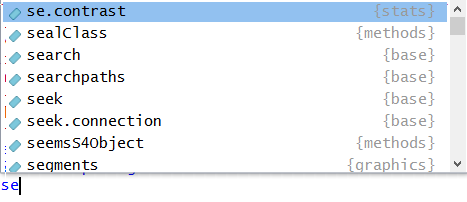
\includegraphics[width=6.49in]{./imagenes/2_function_tab}

Escribir una letra más (e.g. ``q'') reduce la lista de opciones y la
función seq deberá ya ser visible en ellas. Luego basta con oprimir la
tecla Enter para elegir la función seq.

El resultado de utilizar una función se puede también asignar a un
objeto. Esto será de gran utilidad a la hora de trabajar en R.

\begin{Shaded}
\begin{Highlighting}[]
\NormalTok{secuencia_del_1_al_}\DecValTok{100}\NormalTok{ <-}\StringTok{ }\KeywordTok{seq}\NormalTok{(}\DataTypeTok{from=}\DecValTok{1}\NormalTok{,}\DataTypeTok{to=}\DecValTok{100}\NormalTok{)}
\end{Highlighting}
\end{Shaded}

En la sección superior derecha de nuestro ambiente de RStudio ya deben
existir dos objetos cargados en el espacio de trabajo:
``esta\_operacion\_es\_sumamente\_larga'' y
``secuencia\_del\_1\_al\_100''. Estos ya están cargados en la memoria
RAM de la computadora y R puede acceder a ellos cuando se les solicite
utilizando su nombre.

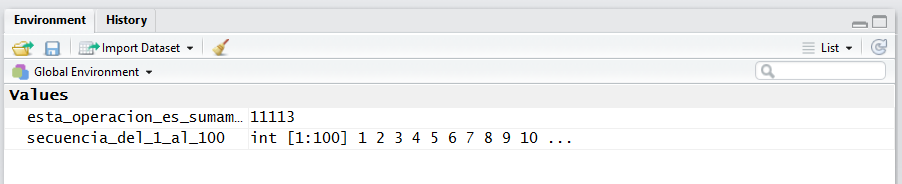
\includegraphics[width=12.53in]{./imagenes/3_espacio_trabajo}


\includegraphics{./imagenes/manicule2.jpg} ¿Por qué no funciona el
siguiente código? Modifícalo hasta que cada instrucción funcione.

library(tidyverse)

ggplot(dota = mpg) + geom\_point(mapping = aes(x = displ, y = hwy))

fliter(mpg, cyl = 8)

filter(diamond, carat \textgreater{} 3)

\subsection{Scripts en R}\label{scripts-en-r}

Se puede escribir código de R en cualquier procesador de texto, por
ejemplo en word. La conveniencia de tener un procesador de texto dentro
de tu ambiente de trabajo (RStudio) es que te permite mandar las
instrucciones diréctamente a la consola para su ejecución.

En un script el símbolo \# le indica a R que esa línea es un comentario.
Los comentarios no se ejecutan y sirven para tener notas para nosotros
mismos sobre el código que estamos desarrollando. Cuando una línea de
texto es un comentario, será de color verde.

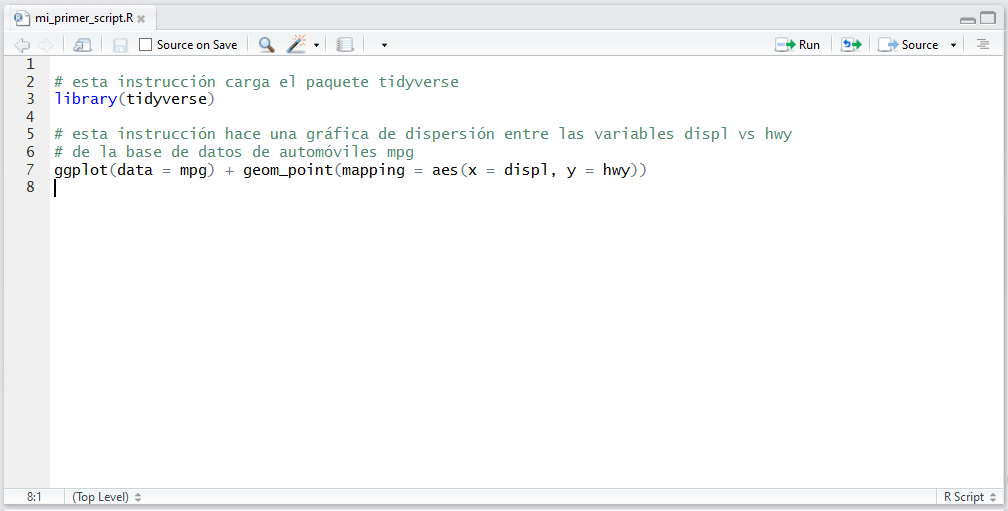
\includegraphics[width=14in]{./imagenes/4_primer_script}

Para ejecutar el código que se encuentra en un script se pueden utilizar
las teclas: Ctrl/Cmd (mac) + Enter o el botón ``Run'' que se encuentra
en la esquina superior derecha de la ventana de scripts. En un script
puedes correr una línea en particular (primero la eliges con el mouse,
botón izquierdo). También puedes correr una selección de tu script, para
esto sólo debes elegir una sección de tu código dejando apretado el
botón derecho del mouse o con la tecla shift y las flechas del teclado;
análogo a como se hace en word.

\subsection{Diagnósticos de RStudio}\label{diagnosticos-de-rstudio}

Como se sabe que R es tan moléstamente quisquilloso, RStudio tiene
integrado un detector de errores de sintaxis.

Un error tremendamente común es que siempre que se abran paréntesis, se
deben cerrar (). Por ejemplo a la hora de usar alguna función. Si
RStudio detecta que en una línea hay paréntesis sin pareja la marcará
con una cruz roja.

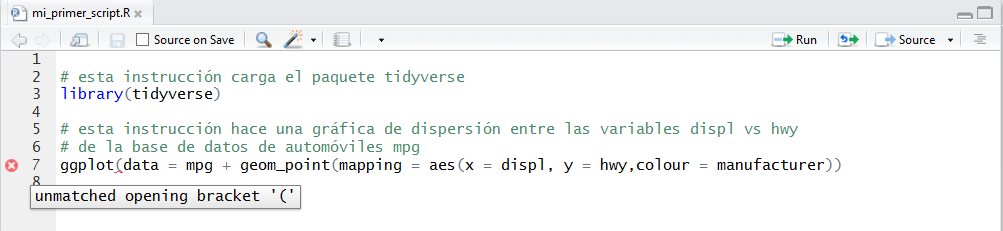
\includegraphics[width=13.93in]{./imagenes/5_unmatched_bracket}

Por supuesto existen muchísimos posibles errores en R. Si se comete
alguno RStudio tratará de informarte sobre la naturaleza del error,
basta con colocar el puntero del mouse sobre la cruz roja para ver esta
nota.

\subsection{Operadores relacionales}\label{operadores-relacionales}

Sirven para comparar dos cantidades. Regresan \textbf{TRUE} si la
comparación es cierta y \textbf{FALSE} en otro caso.

Ejemplos:

\begin{Shaded}
\begin{Highlighting}[]
\DecValTok{5} \OperatorTok{==}\StringTok{ }\DecValTok{5} \CommentTok{# Notar que se pone doble igualdad para comparar dos cantidades}
\end{Highlighting}
\end{Shaded}

\begin{verbatim}
## [1] TRUE
\end{verbatim}

\begin{Shaded}
\begin{Highlighting}[]
\DecValTok{5} \OperatorTok{>}\StringTok{ }\DecValTok{6}
\end{Highlighting}
\end{Shaded}

\begin{verbatim}
## [1] FALSE
\end{verbatim}

\begin{Shaded}
\begin{Highlighting}[]
\DecValTok{5} \OperatorTok{<}\StringTok{ }\DecValTok{6}
\end{Highlighting}
\end{Shaded}

\begin{verbatim}
## [1] TRUE
\end{verbatim}

\begin{Shaded}
\begin{Highlighting}[]
\DecValTok{6} \OperatorTok{>=}\StringTok{ }\DecValTok{3}
\end{Highlighting}
\end{Shaded}

\begin{verbatim}
## [1] TRUE
\end{verbatim}

\begin{Shaded}
\begin{Highlighting}[]
\DecValTok{6} \OperatorTok{<=}\StringTok{ }\FloatTok{3.4}
\end{Highlighting}
\end{Shaded}

\begin{verbatim}
## [1] FALSE
\end{verbatim}

\begin{Shaded}
\begin{Highlighting}[]
\CommentTok{# Otro operador muy útil para ver si un elemento se encuentra en un vector}
\KeywordTok{c}\NormalTok{(}\DecValTok{1}\NormalTok{, }\DecValTok{2}\NormalTok{, }\DecValTok{3}\NormalTok{) }\CommentTok{# Formando un vector que contiene los números 1, 2, 3}
\end{Highlighting}
\end{Shaded}

\begin{verbatim}
## [1] 1 2 3
\end{verbatim}

\begin{Shaded}
\begin{Highlighting}[]
\DecValTok{5} \OperatorTok\StringTok{ }\KeywordTok{c}\NormalTok{(}\DecValTok{1}\NormalTok{, }\DecValTok{2}\NormalTok{, }\DecValTok{3}\NormalTok{)}
\end{Highlighting}
\end{Shaded}

\begin{verbatim}
## [1] FALSE
\end{verbatim}

\begin{Shaded}
\begin{Highlighting}[]
\DecValTok{2} \OperatorTok\StringTok{ }\KeywordTok{c}\NormalTok{(}\DecValTok{1}\NormalTok{, }\DecValTok{2}\NormalTok{, }\DecValTok{3}\NormalTok{)}
\end{Highlighting}
\end{Shaded}

\begin{verbatim}
## [1] TRUE
\end{verbatim}

\subsection{Operadores booleanos}\label{operadores-booleanos}

Sirven para comparar dos expresiones como las anteriores:

El operador \textbf{y} (\&) regresa verdadero si las dos expresiones que
recibe son verdaderas y falso en otro caso.

\begin{Shaded}
\begin{Highlighting}[]
\NormalTok{(}\DecValTok{5} \OperatorTok{>}\StringTok{ }\DecValTok{6}\NormalTok{) }\OperatorTok{&}\StringTok{ }\NormalTok{(}\DecValTok{7} \OperatorTok{<}\StringTok{ }\DecValTok{8}\NormalTok{) }\CommentTok{# Y: notar que regresa false porque 5 > 6 es falso}
\end{Highlighting}
\end{Shaded}

\begin{verbatim}
## [1] FALSE
\end{verbatim}

\begin{Shaded}
\begin{Highlighting}[]
\NormalTok{(}\DecValTok{5} \OperatorTok{<}\StringTok{ }\DecValTok{6}\NormalTok{) }\OperatorTok{&}\StringTok{ }\NormalTok{(}\DecValTok{7} \OperatorTok{<}\StringTok{ }\DecValTok{8}\NormalTok{)}
\end{Highlighting}
\end{Shaded}

\begin{verbatim}
## [1] TRUE
\end{verbatim}

\begin{Shaded}
\begin{Highlighting}[]
\NormalTok{(}\DecValTok{5} \OperatorTok{>}\StringTok{ }\DecValTok{6}\NormalTok{) }\OperatorTok{&}\StringTok{ }\NormalTok{(}\DecValTok{7} \OperatorTok{>}\StringTok{ }\DecValTok{8}\NormalTok{)}
\end{Highlighting}
\end{Shaded}

\begin{verbatim}
## [1] FALSE
\end{verbatim}

El operador \textbf{o} (\textbar{}) regresa verdadero si \textbf{alguna}
de las expresiones que recibe es verdadera y falso en otro caso.

\begin{Shaded}
\begin{Highlighting}[]
\NormalTok{(}\DecValTok{5} \OperatorTok{>}\StringTok{ }\DecValTok{6}\NormalTok{) }\OperatorTok{|}\StringTok{ }\NormalTok{(}\DecValTok{7} \OperatorTok{<}\StringTok{ }\DecValTok{8}\NormalTok{) }\CommentTok{# O: notar que regresa true conque alguna de las expresiones sea verdadera}
\end{Highlighting}
\end{Shaded}

\begin{verbatim}
## [1] TRUE
\end{verbatim}

\begin{Shaded}
\begin{Highlighting}[]
\NormalTok{(}\DecValTok{5} \OperatorTok{<}\StringTok{ }\DecValTok{6}\NormalTok{) }\OperatorTok{|}\StringTok{ }\NormalTok{(}\DecValTok{7} \OperatorTok{<}\StringTok{ }\DecValTok{8}\NormalTok{)}
\end{Highlighting}
\end{Shaded}

\begin{verbatim}
## [1] TRUE
\end{verbatim}

\begin{Shaded}
\begin{Highlighting}[]
\NormalTok{(}\DecValTok{5} \OperatorTok{>}\StringTok{ }\DecValTok{6}\NormalTok{) }\OperatorTok{|}\StringTok{ }\NormalTok{(}\DecValTok{7} \OperatorTok{>}\StringTok{ }\DecValTok{8}\NormalTok{)}
\end{Highlighting}
\end{Shaded}

\begin{verbatim}
## [1] FALSE
\end{verbatim}

El operador lógico \textbf{no} (! regresa verdadero si la expresión que
recibe es falsa y viceversa)

\begin{Shaded}
\begin{Highlighting}[]
\DecValTok{5} \OperatorTok{>}\StringTok{ }\DecValTok{6}
\end{Highlighting}
\end{Shaded}

\begin{verbatim}
## [1] FALSE
\end{verbatim}

\begin{Shaded}
\begin{Highlighting}[]
\OperatorTok{!}\NormalTok{(}\DecValTok{5} \OperatorTok{>}\StringTok{ }\DecValTok{6}\NormalTok{)}
\end{Highlighting}
\end{Shaded}

\begin{verbatim}
## [1] TRUE
\end{verbatim}


\includegraphics{./imagenes/manicule2.jpg} Evalúa una a una las
siguientes expresiones y explica por qué da TRUE o FALSE. Sugerencia:
compréndelas una a una y en orden.

\begin{Shaded}
\begin{Highlighting}[]
\DecValTok{5} \OperatorTok{<}\StringTok{ }\DecValTok{7}
\OperatorTok{!}\NormalTok{(}\DecValTok{5} \OperatorTok{<}\StringTok{ }\DecValTok{7}\NormalTok{)}
\DecValTok{5} \OperatorTok{>}\StringTok{ }\DecValTok{6}
\DecValTok{6} \OperatorTok{<=}\StringTok{ }\DecValTok{6}
\DecValTok{6} \OperatorTok{>=}\StringTok{ }\DecValTok{6}
\OperatorTok{!}\NormalTok{(}\DecValTok{5} \OperatorTok{<}\StringTok{ }\DecValTok{7}\NormalTok{) }\OperatorTok{&}\StringTok{ }\NormalTok{(}\DecValTok{5} \OperatorTok{>}\StringTok{ }\DecValTok{6}\NormalTok{)}
\NormalTok{(}\OperatorTok{!}\NormalTok{(}\DecValTok{5} \OperatorTok{<}\StringTok{ }\DecValTok{7}\NormalTok{) }\OperatorTok{&}\StringTok{ }\NormalTok{(}\DecValTok{5} \OperatorTok{>}\StringTok{ }\DecValTok{6}\NormalTok{)) }\OperatorTok{|}\StringTok{ }\NormalTok{(}\DecValTok{6} \OperatorTok{<=}\StringTok{ }\DecValTok{6}\NormalTok{)}
\OperatorTok{!}\NormalTok{(}\DecValTok{5} \OperatorTok{<}\StringTok{ }\DecValTok{7}\NormalTok{) }\OperatorTok{&}\StringTok{ }\NormalTok{((}\DecValTok{5} \OperatorTok{>}\StringTok{ }\DecValTok{6}\NormalTok{) }\OperatorTok{|}\StringTok{ }\NormalTok{(}\DecValTok{6} \OperatorTok{<=}\StringTok{ }\DecValTok{6}\NormalTok{))}
\end{Highlighting}
\end{Shaded}

\section{El paquete dplyr (instalado con el
tidyverse)}\label{el-paquete-dplyr-instalado-con-el-tidyverse}

\begin{Shaded}
\begin{Highlighting}[]
\CommentTok{# Cargando el paquete}
\KeywordTok{library}\NormalTok{(}\StringTok{"tidyverse"}\NormalTok{)}
\end{Highlighting}
\end{Shaded}

Un data frame se compone de \textbf{registros} (renglones) y
\textbf{campos o variables} (columnas):

\begin{figure}
\centering
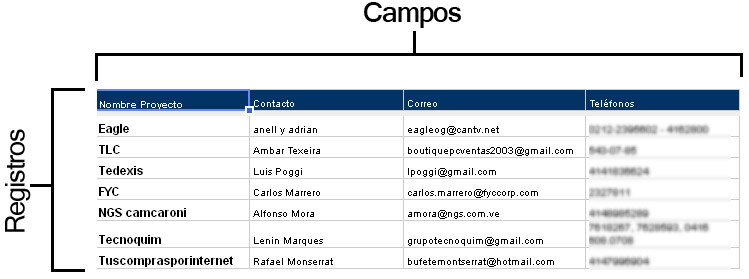
\includegraphics{imagenes/campos_registros.jpg}
\caption{}
\end{figure}

Con \textbf{dplyr} se podrán realizar acciones muy útiles como las
siguientes:

\begin{enumerate}
\def\labelenumi{\arabic{enumi}.}
\tightlist
\item
  \textbf{Seleccionar} campos de un data frame
\item
  \textbf{Filtrar} registros de un data frame que cumplan cierta
  condición.
\item
  \textbf{Ordenar} registros de acurdo a su valor en ciertos campos.
\item
  \textbf{Crear} nuevas columnas a partir de los valores de las
  preexistentes
\item
  \textbf{Calcular resúmenes} de \textbf{agregados} de datos (como las
  tablas dinámicas en Excel).
\item
  \textbf{Unir tablas} de acuerdo a sus valores en ciertos campos (se
  verá más adelante).
\end{enumerate}

\subsection{1. Seleccionar campos de un data frame: select(df,
columnas\_a\_seleccionar)}\label{seleccionar-campos-de-un-data-frame-selectdf-columnas_a_seleccionar}

\begin{Shaded}
\begin{Highlighting}[]
\CommentTok{# Usaremos el data frame diamonds cargado con "tidyverse"}
\KeywordTok{glimpse}\NormalTok{(diamonds)}
\end{Highlighting}
\end{Shaded}

\begin{verbatim}
## Observations: 53,940
## Variables: 10
## $ carat   <dbl> 0.23, 0.21, 0.23, 0.29, 0.31, 0.24, 0.24, 0.26, 0.22, ...
## $ cut     <ord> Ideal, Premium, Good, Premium, Good, Very Good, Very G...
## $ color   <ord> E, E, E, I, J, J, I, H, E, H, J, J, F, J, E, E, I, J, ...
## $ clarity <ord> SI2, SI1, VS1, VS2, SI2, VVS2, VVS1, SI1, VS2, VS1, SI...
## $ depth   <dbl> 61.5, 59.8, 56.9, 62.4, 63.3, 62.8, 62.3, 61.9, 65.1, ...
## $ table   <dbl> 55, 61, 65, 58, 58, 57, 57, 55, 61, 61, 55, 56, 61, 54...
## $ price   <int> 326, 326, 327, 334, 335, 336, 336, 337, 337, 338, 339,...
## $ x       <dbl> 3.95, 3.89, 4.05, 4.20, 4.34, 3.94, 3.95, 4.07, 3.87, ...
## $ y       <dbl> 3.98, 3.84, 4.07, 4.23, 4.35, 3.96, 3.98, 4.11, 3.78, ...
## $ z       <dbl> 2.43, 2.31, 2.31, 2.63, 2.75, 2.48, 2.47, 2.53, 2.49, ...
\end{verbatim}

\begin{Shaded}
\begin{Highlighting}[]
\CommentTok{# View(diamonds) # Para ver el data frame en formato de Excel.}

\NormalTok{diamonds_columnas_selectas <-}\StringTok{ }\KeywordTok{select}\NormalTok{(diamonds, carat, cut)}
\NormalTok{diamonds_columnas_selectas}
\end{Highlighting}
\end{Shaded}

\begin{verbatim}
## # A tibble: 53,940 x 2
##    carat cut      
##    <dbl> <ord>    
##  1 0.23  Ideal    
##  2 0.21  Premium  
##  3 0.23  Good     
##  4 0.290 Premium  
##  5 0.31  Good     
##  6 0.24  Very Good
##  7 0.24  Very Good
##  8 0.26  Very Good
##  9 0.22  Fair     
## 10 0.23  Very Good
## # ... with 53,930 more rows
\end{verbatim}

\begin{Shaded}
\begin{Highlighting}[]
\CommentTok{# Otras maneras de seleccionar columnas:}
\KeywordTok{select}\NormalTok{(diamonds, }\KeywordTok{starts_with}\NormalTok{(}\StringTok{"c"}\NormalTok{))}
\end{Highlighting}
\end{Shaded}

\begin{verbatim}
## # A tibble: 53,940 x 4
##    carat cut       color clarity
##    <dbl> <ord>     <ord> <ord>  
##  1 0.23  Ideal     E     SI2    
##  2 0.21  Premium   E     SI1    
##  3 0.23  Good      E     VS1    
##  4 0.290 Premium   I     VS2    
##  5 0.31  Good      J     SI2    
##  6 0.24  Very Good J     VVS2   
##  7 0.24  Very Good I     VVS1   
##  8 0.26  Very Good H     SI1    
##  9 0.22  Fair      E     VS2    
## 10 0.23  Very Good H     VS1    
## # ... with 53,930 more rows
\end{verbatim}

\begin{Shaded}
\begin{Highlighting}[]
\KeywordTok{select}\NormalTok{(diamonds, }\KeywordTok{contains}\NormalTok{(}\StringTok{"able"}\NormalTok{))}
\end{Highlighting}
\end{Shaded}

\begin{verbatim}
## # A tibble: 53,940 x 1
##    table
##    <dbl>
##  1    55
##  2    61
##  3    65
##  4    58
##  5    58
##  6    57
##  7    57
##  8    55
##  9    61
## 10    61
## # ... with 53,930 more rows
\end{verbatim}

\begin{Shaded}
\begin{Highlighting}[]
\KeywordTok{select}\NormalTok{(diamonds, }\OperatorTok{-}\NormalTok{carat, }\OperatorTok{-}\NormalTok{cut, }\OperatorTok{-}\NormalTok{color)}
\end{Highlighting}
\end{Shaded}

\begin{verbatim}
## # A tibble: 53,940 x 7
##    clarity depth table price     x     y     z
##    <ord>   <dbl> <dbl> <int> <dbl> <dbl> <dbl>
##  1 SI2      61.5    55   326  3.95  3.98  2.43
##  2 SI1      59.8    61   326  3.89  3.84  2.31
##  3 VS1      56.9    65   327  4.05  4.07  2.31
##  4 VS2      62.4    58   334  4.2   4.23  2.63
##  5 SI2      63.3    58   335  4.34  4.35  2.75
##  6 VVS2     62.8    57   336  3.94  3.96  2.48
##  7 VVS1     62.3    57   336  3.95  3.98  2.47
##  8 SI1      61.9    55   337  4.07  4.11  2.53
##  9 VS2      65.1    61   337  3.87  3.78  2.49
## 10 VS1      59.4    61   338  4     4.05  2.39
## # ... with 53,930 more rows
\end{verbatim}


\includegraphics{./imagenes/manicule2.jpg} Crea un data frame nuevo a
partir de diamonds con las columnas carat, x, y, z únicamente.

\subsection{2. Filtrar registros de un data frame que cumplen cierta
condición: filter(df,
condiciones)}\label{filtrar-registros-de-un-data-frame-que-cumplen-cierta-condicion-filterdf-condiciones}

\begin{Shaded}
\begin{Highlighting}[]
\NormalTok{diamonds_registros_selectos <-}\StringTok{ }\KeywordTok{filter}\NormalTok{(diamonds, cut }\OperatorTok{==}\StringTok{ "Ideal"}\NormalTok{, x }\OperatorTok{>}\StringTok{ }\DecValTok{4}\NormalTok{)}
\NormalTok{diamonds_registros_selectos}
\end{Highlighting}
\end{Shaded}

\begin{verbatim}
## # A tibble: 21,449 x 10
##    carat cut   color clarity depth table price     x     y     z
##    <dbl> <ord> <ord> <ord>   <dbl> <dbl> <int> <dbl> <dbl> <dbl>
##  1  0.31 Ideal J     SI2      62.2    54   344  4.35  4.37  2.71
##  2  0.3  Ideal I     SI2      62      54   348  4.31  4.34  2.68
##  3  0.33 Ideal I     SI2      61.8    55   403  4.49  4.51  2.78
##  4  0.33 Ideal I     SI2      61.2    56   403  4.49  4.5   2.75
##  5  0.33 Ideal J     SI1      61.1    56   403  4.49  4.55  2.76
##  6  0.32 Ideal I     SI1      60.9    55   404  4.45  4.48  2.72
##  7  0.3  Ideal I     SI2      61      59   405  4.3   4.33  2.63
##  8  0.35 Ideal I     VS1      60.9    57   552  4.54  4.59  2.78
##  9  0.3  Ideal D     SI1      62.5    57   552  4.29  4.32  2.69
## 10  0.3  Ideal D     SI1      62.1    56   552  4.3   4.33  2.68
## # ... with 21,439 more rows
\end{verbatim}

\begin{Shaded}
\begin{Highlighting}[]
\CommentTok{# Otras maneras de filtrar registros}
\KeywordTok{filter}\NormalTok{(diamonds, cut }\OperatorTok{==}\StringTok{ "Ideal"} \OperatorTok{&}\StringTok{ }\NormalTok{x }\OperatorTok{>}\StringTok{ }\DecValTok{4}\NormalTok{)}
\end{Highlighting}
\end{Shaded}

\begin{verbatim}
## # A tibble: 21,449 x 10
##    carat cut   color clarity depth table price     x     y     z
##    <dbl> <ord> <ord> <ord>   <dbl> <dbl> <int> <dbl> <dbl> <dbl>
##  1  0.31 Ideal J     SI2      62.2    54   344  4.35  4.37  2.71
##  2  0.3  Ideal I     SI2      62      54   348  4.31  4.34  2.68
##  3  0.33 Ideal I     SI2      61.8    55   403  4.49  4.51  2.78
##  4  0.33 Ideal I     SI2      61.2    56   403  4.49  4.5   2.75
##  5  0.33 Ideal J     SI1      61.1    56   403  4.49  4.55  2.76
##  6  0.32 Ideal I     SI1      60.9    55   404  4.45  4.48  2.72
##  7  0.3  Ideal I     SI2      61      59   405  4.3   4.33  2.63
##  8  0.35 Ideal I     VS1      60.9    57   552  4.54  4.59  2.78
##  9  0.3  Ideal D     SI1      62.5    57   552  4.29  4.32  2.69
## 10  0.3  Ideal D     SI1      62.1    56   552  4.3   4.33  2.68
## # ... with 21,439 more rows
\end{verbatim}

\begin{Shaded}
\begin{Highlighting}[]
\KeywordTok{filter}\NormalTok{(diamonds, cut }\OperatorTok{==}\StringTok{ "Ideal"} \OperatorTok{|}\StringTok{ }\NormalTok{x }\OperatorTok{>}\StringTok{ }\DecValTok{4}\NormalTok{)}
\end{Highlighting}
\end{Shaded}

\begin{verbatim}
## # A tibble: 53,546 x 10
##    carat cut       color clarity depth table price     x     y     z
##    <dbl> <ord>     <ord> <ord>   <dbl> <dbl> <int> <dbl> <dbl> <dbl>
##  1 0.23  Ideal     E     SI2      61.5    55   326  3.95  3.98  2.43
##  2 0.23  Good      E     VS1      56.9    65   327  4.05  4.07  2.31
##  3 0.290 Premium   I     VS2      62.4    58   334  4.2   4.23  2.63
##  4 0.31  Good      J     SI2      63.3    58   335  4.34  4.35  2.75
##  5 0.26  Very Good H     SI1      61.9    55   337  4.07  4.11  2.53
##  6 0.3   Good      J     SI1      64      55   339  4.25  4.28  2.73
##  7 0.23  Ideal     J     VS1      62.8    56   340  3.93  3.9   2.46
##  8 0.31  Ideal     J     SI2      62.2    54   344  4.35  4.37  2.71
##  9 0.32  Premium   E     I1       60.9    58   345  4.38  4.42  2.68
## 10 0.3   Ideal     I     SI2      62      54   348  4.31  4.34  2.68
## # ... with 53,536 more rows
\end{verbatim}


\includegraphics{./imagenes/manicule2.jpg} Crea un data frame nuevo a
partir de diamonds que contenga los registros que cumplen la condición:
`\textbf{alguna} de x, y, z es mayor a 3.5'

\subsection{3. Ordenar registros de un data frame por los valores en una
o más variables: arrange(df,
variables\_de\_ordenamiento)}\label{ordenar-registros-de-un-data-frame-por-los-valores-en-una-o-mas-variables-arrangedf-variables_de_ordenamiento}

\begin{Shaded}
\begin{Highlighting}[]
\NormalTok{diamonds_ordenado <-}\StringTok{ }\KeywordTok{arrange}\NormalTok{(diamonds, carat, depth)}
\NormalTok{diamonds_ordenado}
\end{Highlighting}
\end{Shaded}

\begin{verbatim}
## # A tibble: 53,940 x 10
##    carat cut     color clarity depth table price     x     y     z
##    <dbl> <ord>   <ord> <ord>   <dbl> <dbl> <int> <dbl> <dbl> <dbl>
##  1   0.2 Premium E     VS2      59      60   367  3.81  3.78  2.24
##  2   0.2 Premium E     VS2      59.7    62   367  3.84  3.8   2.28
##  3   0.2 Ideal   E     VS2      59.7    55   367  3.86  3.84  2.3 
##  4   0.2 Premium E     VS2      59.8    62   367  3.79  3.77  2.26
##  5   0.2 Premium E     SI2      60.2    62   345  3.79  3.75  2.27
##  6   0.2 Premium E     VS2      61.1    59   367  3.81  3.78  2.32
##  7   0.2 Ideal   D     VS2      61.5    57   367  3.81  3.77  2.33
##  8   0.2 Premium D     VS2      61.7    60   367  3.77  3.72  2.31
##  9   0.2 Ideal   E     VS2      62.2    57   367  3.76  3.73  2.33
## 10   0.2 Premium D     VS2      62.3    60   367  3.73  3.68  2.31
## # ... with 53,930 more rows
\end{verbatim}

\begin{Shaded}
\begin{Highlighting}[]
\CommentTok{# desc(variable): ordena en sentido decreciente (Z-A), (mayor a menor, etc)}
\KeywordTok{arrange}\NormalTok{(diamonds, carat, }\KeywordTok{desc}\NormalTok{(depth))}
\end{Highlighting}
\end{Shaded}

\begin{verbatim}
## # A tibble: 53,940 x 10
##    carat cut       color clarity depth table price     x     y     z
##    <dbl> <ord>     <ord> <ord>   <dbl> <dbl> <int> <dbl> <dbl> <dbl>
##  1   0.2 Very Good E     VS2      63.4    59   367  3.74  3.71  2.36
##  2   0.2 Premium   F     VS2      62.6    59   367  3.73  3.71  2.33
##  3   0.2 Premium   D     VS2      62.3    60   367  3.73  3.68  2.31
##  4   0.2 Ideal     E     VS2      62.2    57   367  3.76  3.73  2.33
##  5   0.2 Premium   D     VS2      61.7    60   367  3.77  3.72  2.31
##  6   0.2 Ideal     D     VS2      61.5    57   367  3.81  3.77  2.33
##  7   0.2 Premium   E     VS2      61.1    59   367  3.81  3.78  2.32
##  8   0.2 Premium   E     SI2      60.2    62   345  3.79  3.75  2.27
##  9   0.2 Premium   E     VS2      59.8    62   367  3.79  3.77  2.26
## 10   0.2 Premium   E     VS2      59.7    62   367  3.84  3.8   2.28
## # ... with 53,930 more rows
\end{verbatim}

\begin{Shaded}
\begin{Highlighting}[]
\KeywordTok{arrange}\NormalTok{(diamonds, }\KeywordTok{desc}\NormalTok{(carat), depth)}
\end{Highlighting}
\end{Shaded}

\begin{verbatim}
## # A tibble: 53,940 x 10
##    carat cut       color clarity depth table price     x     y     z
##    <dbl> <ord>     <ord> <ord>   <dbl> <dbl> <int> <dbl> <dbl> <dbl>
##  1  5.01 Fair      J     I1       65.5    59 18018 10.7  10.5   6.98
##  2  4.5  Fair      J     I1       65.8    58 18531 10.2  10.2   6.72
##  3  4.13 Fair      H     I1       64.8    61 17329 10     9.85  6.43
##  4  4.01 Premium   I     I1       61      61 15223 10.1  10.1   6.17
##  5  4.01 Premium   J     I1       62.5    62 15223 10.0   9.94  6.24
##  6  4    Very Good I     I1       63.3    58 15984 10.0   9.94  6.31
##  7  3.67 Premium   I     I1       62.4    56 16193  9.86  9.81  6.13
##  8  3.65 Fair      H     I1       67.1    53 11668  9.53  9.48  6.38
##  9  3.51 Premium   J     VS2      62.5    59 18701  9.66  9.63  6.03
## 10  3.5  Ideal     H     I1       62.8    57 12587  9.65  9.59  6.03
## # ... with 53,930 more rows
\end{verbatim}


\includegraphics{./imagenes/manicule2.jpg} Crea un data frame nuevo a
partir de diamonds que contenga los registros organizados
alfabéticamente por ``color''``, y por''carat" de manera descendente.

\subsection{4. Crear nuevas variables: mutate(df,
formulas)}\label{crear-nuevas-variables-mutatedf-formulas}

\begin{Shaded}
\begin{Highlighting}[]
\NormalTok{diamonds_nueva_variable <-}\StringTok{ }\KeywordTok{mutate}\NormalTok{(diamonds, }\DataTypeTok{dollars_per_carat =}\NormalTok{ price }\OperatorTok{/}\StringTok{ }\NormalTok{carat)}
\end{Highlighting}
\end{Shaded}


\includegraphics{./imagenes/manicule2.jpg} Crea un data frame nuevo a
partir de diamonds que contenga la variable ``dollars\_per\_carat''
anterior, y la variable ``product'' calculada como \(x \times\) y
\(\times z\).

\subsection{5. Agrupar por ciertas variables: group\_by(data\_frame,
variables) y crear resúmenes por grupo: summarise(data\_frame,
formulas)}\label{agrupar-por-ciertas-variables-group_bydata_frame-variables-y-crear-resumenes-por-grupo-summarisedata_frame-formulas}

\begin{itemize}
\tightlist
\item
  Para crear resúmenes de un data frame se utiliza la función
  \textbf{summarise}.
\item
  Si se agrupan los datos antes (utilizando la función
  \textbf{group\_by}), se pueden crear resúmenes por nivel de las
  variables de agregación (definidas en el group\_by). Esto es análogo a
  las tablas dinámicas en Excel.
\end{itemize}

\begin{Shaded}
\begin{Highlighting}[]
\CommentTok{# Calcular el promedio de depth y la mediana de price y asignarlos a las}
\CommentTok{# variables "promedio_depth" y "mediana_price"}
\NormalTok{diamonds_resumen <-}\StringTok{ }\KeywordTok{summarise}\NormalTok{(diamonds, }\DataTypeTok{promedio_depth =} \KeywordTok{mean}\NormalTok{(depth), }\DataTypeTok{mediana_price =} \KeywordTok{median}\NormalTok{(price))}
\NormalTok{diamonds_resumen}
\end{Highlighting}
\end{Shaded}

\begin{verbatim}
## # A tibble: 1 x 2
##   promedio_depth mediana_price
##            <dbl>         <dbl>
## 1           61.7          2401
\end{verbatim}

\begin{Shaded}
\begin{Highlighting}[]
\CommentTok{# Calcular el promedio de depth y la mediana de price y asignarlos a las variables}
\CommentTok{# "promedio_depth" y "mediana_price", por nivel de "cut"}
\CommentTok{# Primero agrupo por la variable de interés}
\NormalTok{diamonds_agrupado <-}\StringTok{ }\KeywordTok{group_by}\NormalTok{(diamonds, cut)}
\NormalTok{diamonds_agrupado}
\end{Highlighting}
\end{Shaded}

\begin{verbatim}
## # A tibble: 53,940 x 10
## # Groups:   cut [5]
##    carat cut       color clarity depth table price     x     y     z
##    <dbl> <ord>     <ord> <ord>   <dbl> <dbl> <int> <dbl> <dbl> <dbl>
##  1 0.23  Ideal     E     SI2      61.5    55   326  3.95  3.98  2.43
##  2 0.21  Premium   E     SI1      59.8    61   326  3.89  3.84  2.31
##  3 0.23  Good      E     VS1      56.9    65   327  4.05  4.07  2.31
##  4 0.290 Premium   I     VS2      62.4    58   334  4.2   4.23  2.63
##  5 0.31  Good      J     SI2      63.3    58   335  4.34  4.35  2.75
##  6 0.24  Very Good J     VVS2     62.8    57   336  3.94  3.96  2.48
##  7 0.24  Very Good I     VVS1     62.3    57   336  3.95  3.98  2.47
##  8 0.26  Very Good H     SI1      61.9    55   337  4.07  4.11  2.53
##  9 0.22  Fair      E     VS2      65.1    61   337  3.87  3.78  2.49
## 10 0.23  Very Good H     VS1      59.4    61   338  4     4.05  2.39
## # ... with 53,930 more rows
\end{verbatim}

\begin{Shaded}
\begin{Highlighting}[]
\CommentTok{# Y calculo resúmenes para cada nivel de dicha variable}
\NormalTok{diamonds_resumen_por_grupo <-}\StringTok{ }\KeywordTok{summarise}\NormalTok{(diamonds_agrupado, }\DataTypeTok{promedio_depth =} \KeywordTok{mean}\NormalTok{(depth), }\DataTypeTok{mediana_price =} \KeywordTok{median}\NormalTok{(price))}
\NormalTok{diamonds_resumen_por_grupo}
\end{Highlighting}
\end{Shaded}

\begin{verbatim}
## # A tibble: 5 x 3
##   cut       promedio_depth mediana_price
##   <ord>              <dbl>         <dbl>
## 1 Fair                64.0         3282 
## 2 Good                62.4         3050.
## 3 Very Good           61.8         2648 
## 4 Premium             61.3         3185 
## 5 Ideal               61.7         1810
\end{verbatim}

Algunos resúmenes útiles con \emph{summarise} son:

\begin{itemize}
\tightlist
\item
  El mínimo de un campo x: \textbf{min(x)}
\item
  La mediana de un campo x: \textbf{median(x)}
\item
  El máximo de un campo x: \textbf{max(x)}
\item
  El número de registros: \textbf{n()}
\item
  La suma de un campo x: \textbf{sum(x)}
\item
  La desviación estándar de un campo x: \textbf{sd(x)}.
\end{itemize}


\includegraphics{./imagenes/manicule.jpg} \textbf{Tarea:} Crea un data
frame nuevo a partir de diamonds que contenga el número de registros
para cada combinación de valores en las variables ``cut'' y ``color''.


\includegraphics{./imagenes/manicule.jpg} \textbf{Tarea:} Explica las
diferencias que notas entre los data frames obtenidos de:

\begin{Shaded}
\begin{Highlighting}[]
\NormalTok{diamonds_agrupado <-}\StringTok{ }\KeywordTok{group_by}\NormalTok{(diamonds, cut)}
\NormalTok{resultado_}\DecValTok{1}\NormalTok{ <-}\StringTok{ }\KeywordTok{summarise}\NormalTok{(diamonds_agrupado, }\DataTypeTok{promedio_depth =} \KeywordTok{mean}\NormalTok{(depth))}
\NormalTok{resultado_}\DecValTok{2}\NormalTok{ <-}\StringTok{ }\KeywordTok{mutate}\NormalTok{(diamonds_agrupado, }\DataTypeTok{promedio_depth =} \KeywordTok{mean}\NormalTok{(depth))}
\end{Highlighting}
\end{Shaded}


\includegraphics{./imagenes/manicule.jpg} \textbf{Tarea:} Partiendo del
data frame diamonds, crea un data frame nuevo con las siguientes
características:

\begin{enumerate}
\def\labelenumi{\arabic{enumi}.}
\item
  Contenga la variable dollars\_per\_carat = price / carat
\item
  Contenga sólo aquellos registros que cumplen dollars\_per\_carat
  \textless{} 4000
\item
  Esté ordenado en orden descendente por la variable dollars\_per\_carat
\end{enumerate}

\chapter{Transformación-II}\label{transformacion-ii}

\section{¿Qué aprendimos la clase
pasada?}\label{que-aprendimos-la-clase-pasada-1}

\begin{itemize}
\tightlist
\item
  Utilizamos R para saber si comparaciones entre dos cantidades son
  ciertas o no (5 \textgreater{} 6 \#FALSE, 6 == 6 \#TRUE)
\item
  Aprendimos el uso de los operadores y (\&), o (\textbar{}) y no (!):
  (5 \textgreater{} 6) \textbar{} (3 \textless{} 4) \#TRUE
\item
  Aprendimos las funciones básicas para manipular \textbf{tablas de
  datos} (paquete \textbf{dplyr} contenido en el tidyverse):
\end{itemize}

\begin{tabular}{l|l|l}
\hline
Funcionalidad & Función & Interpretación\\
\hline
Seleccionar campos & select(diamonds, carat, cut) & Del data frame diamonds \_\_seleccióname los campos\_\_ carat y cut\\
\hline
Seleccionar registros de acuerdo a un criterio & filter(diamonds, cut == "Ideal" | x > 4) & Del data frame diamonds \_\_seleccióname los registros (filter)\_\_ que cumplen "cut == "Ideal" o (|) "x > 4"\\
\hline
Ordenar registros de acuerdo a uno o más campos & arrange(diamonds, carat, depth) & Del data frame diamonds \_\_ordéname los registros\_\_ primero por carat y luego, los que tengan valores iguales, por depth\\
\hline
Crear nuevas variables & mutate(diamonds, dollars\_per\_carat = price / carat) & Usando el data frame diamonds \_\_créame la nueva columna\_\_ dollars\_per\_carat definida como price / carat\\
\hline
Preparar un data frame para calcular resúmenes por grupo & diamonds\_agrupado <- group\_by(diamonds, cut) & Usando el data frame diamonds, \_\_prepárame los datos\_\_ para calcular resúmenes por valor de la columna cut, y \_\_asigna\_\_ el resultado a la variable diamonds\_agrupado\\
\hline
Calcular resúmenes por grupo & summarise(diamonds\_agrupado, promedio\_depth = mean(depth)) & Usando diamonds agrupado, \_\_calcúlame el resumen\_\_ llamado promedio depth definido como la media de depth\\
\hline
\end{tabular}

En esta clase aprenderemos a:

\begin{itemize}
\tightlist
\item
  Utilizar el operador \textbf{pipeline} para simplificar la aplicación
  de funciones de transformación de datos, una tras otra (recordar la
  tarea, ejercicio 3).
\item
  Miscelánea de funcionalidades avanzadas de transformación de datos:

  \begin{itemize}
  \tightlist
  \item
    \textbf{joins} (uniones de dos o más tablas).
  \item
    El paquete \textbf{tidyr} para transformar la \textbf{estructura} de
    los datos en una tabla.
  \end{itemize}
\item
  Un poco acerca de datos faltantes.
\item
  Leer datos en R.
\end{itemize}

\section{El operador pipeline
\%\textgreater{}\%}\label{el-operador-pipeline}

El ejercicio 3 de la tarea nos introduce a lo tedioso que es aplicar
varias funciones para transformar datos una tras otra sin ayuda. Aquí es
cuando el operador pipeline entra en acción:

Nos permite encadenar operaciones de manera sencilla, comenzando por el
data frame original (diamonds), luego aplicar una transformación, al
resultado aplicar otra y así sucesivamente.

Retomemos el ejemplo de la tarea 3. En lugar de:

\begin{Shaded}
\begin{Highlighting}[]
\NormalTok{diamonds_dollars_per_carat <-}\StringTok{ }\KeywordTok{mutate}\NormalTok{(diamonds, }\DataTypeTok{dollars_per_carat =}\NormalTok{ price }\OperatorTok{/}\StringTok{ }\NormalTok{carat)}
\NormalTok{diamonds_dollars_per_carat}
\end{Highlighting}
\end{Shaded}

\begin{verbatim}
## # A tibble: 53,940 x 11
##    carat cut       color clarity depth table price     x     y     z
##    <dbl> <ord>     <ord> <ord>   <dbl> <dbl> <int> <dbl> <dbl> <dbl>
##  1 0.23  Ideal     E     SI2      61.5    55   326  3.95  3.98  2.43
##  2 0.21  Premium   E     SI1      59.8    61   326  3.89  3.84  2.31
##  3 0.23  Good      E     VS1      56.9    65   327  4.05  4.07  2.31
##  4 0.290 Premium   I     VS2      62.4    58   334  4.2   4.23  2.63
##  5 0.31  Good      J     SI2      63.3    58   335  4.34  4.35  2.75
##  6 0.24  Very Good J     VVS2     62.8    57   336  3.94  3.96  2.48
##  7 0.24  Very Good I     VVS1     62.3    57   336  3.95  3.98  2.47
##  8 0.26  Very Good H     SI1      61.9    55   337  4.07  4.11  2.53
##  9 0.22  Fair      E     VS2      65.1    61   337  3.87  3.78  2.49
## 10 0.23  Very Good H     VS1      59.4    61   338  4     4.05  2.39
## # ... with 53,930 more rows, and 1 more variable: dollars_per_carat <dbl>
\end{verbatim}

\begin{Shaded}
\begin{Highlighting}[]
\NormalTok{diamonds_dollars_per_carat_filtrado <-}\StringTok{ }\KeywordTok{filter}\NormalTok{(diamonds_dollars_per_carat, dollars_per_carat }\OperatorTok{<}\StringTok{ }\DecValTok{4000}\NormalTok{)}
\NormalTok{diamonds_dollars_per_carat_filtrado}
\end{Highlighting}
\end{Shaded}

\begin{verbatim}
## # A tibble: 32,083 x 11
##    carat cut       color clarity depth table price     x     y     z
##    <dbl> <ord>     <ord> <ord>   <dbl> <dbl> <int> <dbl> <dbl> <dbl>
##  1 0.23  Ideal     E     SI2      61.5    55   326  3.95  3.98  2.43
##  2 0.21  Premium   E     SI1      59.8    61   326  3.89  3.84  2.31
##  3 0.23  Good      E     VS1      56.9    65   327  4.05  4.07  2.31
##  4 0.290 Premium   I     VS2      62.4    58   334  4.2   4.23  2.63
##  5 0.31  Good      J     SI2      63.3    58   335  4.34  4.35  2.75
##  6 0.24  Very Good J     VVS2     62.8    57   336  3.94  3.96  2.48
##  7 0.24  Very Good I     VVS1     62.3    57   336  3.95  3.98  2.47
##  8 0.26  Very Good H     SI1      61.9    55   337  4.07  4.11  2.53
##  9 0.22  Fair      E     VS2      65.1    61   337  3.87  3.78  2.49
## 10 0.23  Very Good H     VS1      59.4    61   338  4     4.05  2.39
## # ... with 32,073 more rows, and 1 more variable: dollars_per_carat <dbl>
\end{verbatim}

\begin{Shaded}
\begin{Highlighting}[]
\NormalTok{diamonds_dollars_per_carat_filtrado_ordenado <-}\StringTok{ }\KeywordTok{arrange}\NormalTok{(diamonds_dollars_per_carat_filtrado, }\KeywordTok{desc}\NormalTok{(dollars_per_carat))}
\NormalTok{diamonds_dollars_per_carat_filtrado_ordenado}
\end{Highlighting}
\end{Shaded}

\begin{verbatim}
## # A tibble: 32,083 x 11
##    carat cut       color clarity depth table price     x     y     z
##    <dbl> <ord>     <ord> <ord>   <dbl> <dbl> <int> <dbl> <dbl> <dbl>
##  1  1.05 Very Good J     SI1      62.5    58  4199  6.47  6.52  4.06
##  2  0.92 Very Good E     SI2      63.2    54  3679  6.29  6.25  3.96
##  3  0.92 Premium   E     SI2      61.8    59  3679  6.19  6.11  3.8 
##  4  0.91 Premium   E     SI2      61.1    59  3639  6.24  6.2   3.8 
##  5  0.91 Premium   E     SI2      62.8    61  3639  6.09  6.07  3.82
##  6  0.9  Premium   E     SI2      62.6    60  3599  6.18  6.09  3.84
##  7  0.9  Premium   E     SI2      62.2    60  3599  6.19  6.15  3.84
##  8  0.9  Ideal     E     SI2      62      55  3599  6.23  6.15  3.84
##  9  1.51 Premium   H     I1       61.9    58  6038  7.39  7.34  4.56
## 10  0.74 Fair      G     VVS2     65.2    58  2959  5.7   5.6   3.69
## # ... with 32,073 more rows, and 1 more variable: dollars_per_carat <dbl>
\end{verbatim}

El ejemplo de la tarea 3 queda:

\begin{Shaded}
\begin{Highlighting}[]
\NormalTok{diamonds }\OperatorTok\StringTok{ }\CommentTok{# Comenzando con el df diamonds:}
\StringTok{  }\KeywordTok{mutate}\NormalTok{(}\DataTypeTok{dollars_per_carat =}\NormalTok{ price }\OperatorTok{/}\StringTok{ }\NormalTok{carat) }\OperatorTok\StringTok{ }\CommentTok{# Calcúlame la variable dollars per carat ... LUEGO}
\StringTok{  }\KeywordTok{filter}\NormalTok{(dollars_per_carat }\OperatorTok{<}\StringTok{ }\DecValTok{4000}\NormalTok{) }\OperatorTok\StringTok{ }\CommentTok{# Seleccióname los registros en que la variable dollars_per_carat < 4000 LUEGO}
\StringTok{  }\KeywordTok{arrange}\NormalTok{(}\KeywordTok{desc}\NormalTok{(dollars_per_carat)) }\CommentTok{# Ordéname en orden descendente por la variable dollars per carat}
\end{Highlighting}
\end{Shaded}

\begin{verbatim}
## # A tibble: 32,083 x 11
##    carat cut       color clarity depth table price     x     y     z
##    <dbl> <ord>     <ord> <ord>   <dbl> <dbl> <int> <dbl> <dbl> <dbl>
##  1  1.05 Very Good J     SI1      62.5    58  4199  6.47  6.52  4.06
##  2  0.92 Very Good E     SI2      63.2    54  3679  6.29  6.25  3.96
##  3  0.92 Premium   E     SI2      61.8    59  3679  6.19  6.11  3.8 
##  4  0.91 Premium   E     SI2      61.1    59  3639  6.24  6.2   3.8 
##  5  0.91 Premium   E     SI2      62.8    61  3639  6.09  6.07  3.82
##  6  0.9  Premium   E     SI2      62.6    60  3599  6.18  6.09  3.84
##  7  0.9  Premium   E     SI2      62.2    60  3599  6.19  6.15  3.84
##  8  0.9  Ideal     E     SI2      62      55  3599  6.23  6.15  3.84
##  9  1.51 Premium   H     I1       61.9    58  6038  7.39  7.34  4.56
## 10  0.74 Fair      G     VVS2     65.2    58  2959  5.7   5.6   3.69
## # ... with 32,073 more rows, and 1 more variable: dollars_per_carat <dbl>
\end{verbatim}

Podemos también asignar el resultado de TODAS las transformaciones
anteriores a una variable

\begin{Shaded}
\begin{Highlighting}[]
\NormalTok{diamonds_transformado_}\DecValTok{1}\NormalTok{ <-}\StringTok{ }\NormalTok{diamonds }\OperatorTok
\StringTok{  }\KeywordTok{mutate}\NormalTok{(}\DataTypeTok{dollars_per_carat =}\NormalTok{ price }\OperatorTok{/}\StringTok{ }\NormalTok{carat) }\OperatorTok
\StringTok{  }\KeywordTok{filter}\NormalTok{(dollars_per_carat }\OperatorTok{<}\StringTok{ }\DecValTok{4000}\NormalTok{) }\OperatorTok
\StringTok{  }\KeywordTok{arrange}\NormalTok{(}\KeywordTok{desc}\NormalTok{(dollars_per_carat))}
\NormalTok{diamonds_transformado_}\DecValTok{1}
\end{Highlighting}
\end{Shaded}

\begin{verbatim}
## # A tibble: 32,083 x 11
##    carat cut       color clarity depth table price     x     y     z
##    <dbl> <ord>     <ord> <ord>   <dbl> <dbl> <int> <dbl> <dbl> <dbl>
##  1  1.05 Very Good J     SI1      62.5    58  4199  6.47  6.52  4.06
##  2  0.92 Very Good E     SI2      63.2    54  3679  6.29  6.25  3.96
##  3  0.92 Premium   E     SI2      61.8    59  3679  6.19  6.11  3.8 
##  4  0.91 Premium   E     SI2      61.1    59  3639  6.24  6.2   3.8 
##  5  0.91 Premium   E     SI2      62.8    61  3639  6.09  6.07  3.82
##  6  0.9  Premium   E     SI2      62.6    60  3599  6.18  6.09  3.84
##  7  0.9  Premium   E     SI2      62.2    60  3599  6.19  6.15  3.84
##  8  0.9  Ideal     E     SI2      62      55  3599  6.23  6.15  3.84
##  9  1.51 Premium   H     I1       61.9    58  6038  7.39  7.34  4.56
## 10  0.74 Fair      G     VVS2     65.2    58  2959  5.7   5.6   3.69
## # ... with 32,073 more rows, and 1 more variable: dollars_per_carat <dbl>
\end{verbatim}

Otro ejemplo:

\begin{itemize}
\tightlist
\item
  Por combinación de cut y color,
\item
  Calcular el mínimo de x, y también el máximo de y.
\item
  Al resultado ordenarlo por color de manera descendente.
\end{itemize}

\begin{Shaded}
\begin{Highlighting}[]
\NormalTok{diamonds_transformado_}\DecValTok{2}\NormalTok{ <-}\StringTok{ }\NormalTok{diamonds }\OperatorTok
\StringTok{  }\CommentTok{# Primero agrupo por combinación de cut y color, ya que lo necesito para calcular}
\StringTok{  }\CommentTok{# los resúmenes por grupo}
\StringTok{  }\KeywordTok{group_by}\NormalTok{(cut, color) }\OperatorTok
\StringTok{  }\CommentTok{# Luego calculo los resúmenes por grupo}
\StringTok{  }\KeywordTok{summarise}\NormalTok{(}\DataTypeTok{minimo_x =} \KeywordTok{min}\NormalTok{(x), }\DataTypeTok{maximo_y =} \KeywordTok{max}\NormalTok{(y)) }\OperatorTok
\StringTok{  }\CommentTok{# Finalmente ordeno por color}
\StringTok{  }\KeywordTok{arrange}\NormalTok{(}\KeywordTok{desc}\NormalTok{(color))}
\NormalTok{diamonds_transformado_}\DecValTok{2}
\end{Highlighting}
\end{Shaded}

\begin{verbatim}
## # A tibble: 35 x 4
## # Groups:   cut [5]
##    cut       color minimo_x maximo_y
##    <ord>     <ord>    <dbl>    <dbl>
##  1 Fair      J         4.24    10.5 
##  2 Good      J         4.22     9.19
##  3 Very Good J         3.94     8.93
##  4 Premium   J         4.22     9.94
##  5 Ideal     J         3.93     9.2 
##  6 Fair      I         4.62     9.02
##  7 Good      I         4.19     9.31
##  8 Very Good I         3.95     9.94
##  9 Premium   I         3.97    10.1 
## 10 Ideal     I         3.94     9.42
## # ... with 25 more rows
\end{verbatim}

\section{Miscelánea de funcionalidades avanzadas de transformación de
datos}\label{miscelanea-de-funcionalidades-avanzadas-de-transformacion-de-datos}

Con \textbf{dplyr}:

\begin{enumerate}
\def\labelenumi{\arabic{enumi}.}
\tightlist
\item
  Realizar \textbf{joins} entre dos tablas.
\end{enumerate}

Con \textbf{tidyr}:

\begin{enumerate}
\def\labelenumi{\arabic{enumi}.}
\setcounter{enumi}{1}
\tightlist
\item
  \textbf{Spread}: transformar registros en campos
\item
  \textbf{Gather}: transformar campos en registros
\item
  \textbf{Separate}: separar variables
\end{enumerate}

\subsection{1. Joins: inner\_join(df1, df2,
columnas\_a\_seleccionar)}\label{joins-inner_joindf1-df2-columnas_a_seleccionar}

Es común encontrarse tablas que hacer referencia la una a la otra, por
ejemplo:

\begin{table}

\caption{\label{tab:unnamed-chunk-29}Tipos de caracter}
\centering
\begin{tabular}[t]{r|l}
\hline
id & tipo\\
\hline
1 & letra\\
\hline
2 & número\\
\hline
3 & caracter especial\\
\hline
\end{tabular}
\end{table}

\begin{table}

\caption{\label{tab:unnamed-chunk-29}Caracteres}
\centering
\begin{tabular}[t]{c|c|c}
\hline
id & caracter & tipo\_caracter\_id\\
\hline
1 & a & 1\\
\hline
2 & 2 & 2\\
\hline
3 & 3 & 2\\
\hline
4 & 1 & 2\\
\hline
5 & z & 1\\
\hline
6 & 5 & 2\\
\hline
7 & m & 1\\
\hline
8 & 7 & 2\\
\hline
9 & s & 1\\
\hline
10 & x & 1\\
\hline
\end{tabular}
\end{table}

Para asociar a cada caracter su tipo, podemos utilizar una funcionalidad
llamada \textbf{join}, que básicamente asocia registros de dos tablas
usando campos en común.

\begin{Shaded}
\begin{Highlighting}[]
\CommentTok{# Definiendo las tablas anteriores (normalmente estas tablas se leerán de archivos}
\CommentTok{# CSV o bases de datos como se verá en esta clase).}

\NormalTok{tipos_caracter <-}\StringTok{ }\KeywordTok{data_frame}\NormalTok{(}
  \DataTypeTok{id =} \KeywordTok{c}\NormalTok{(}\DecValTok{1}\NormalTok{, }\DecValTok{2}\NormalTok{, }\DecValTok{3}\NormalTok{),}
  \DataTypeTok{tipo =} \KeywordTok{c}\NormalTok{(}\StringTok{"letra"}\NormalTok{, }\StringTok{"número", "}\NormalTok{caracter especial}\StringTok{")}
\StringTok{)}
\StringTok{tipos_caracter}
\end{Highlighting}
\end{Shaded}

\begin{verbatim}
## # A tibble: 3 x 2
##      id tipo             
##   <dbl> <chr>            
## 1     1 letra            
## 2     2 número           
## 3     3 caracter especial
\end{verbatim}

\begin{Shaded}
\begin{Highlighting}[]
\NormalTok{caracteres <-}\StringTok{ }\KeywordTok{data_frame}\NormalTok{(}
  \DataTypeTok{id =} \DecValTok{1}\OperatorTok{:}\DecValTok{10}\NormalTok{,}
  \DataTypeTok{caracter =} \KeywordTok{c}\NormalTok{(}\StringTok{"a"}\NormalTok{, }\StringTok{"2"}\NormalTok{, }\StringTok{"3"}\NormalTok{, }\StringTok{"1"}\NormalTok{, }\StringTok{"z"}\NormalTok{, }\StringTok{"5"}\NormalTok{, }\StringTok{"m"}\NormalTok{, }\StringTok{"7"}\NormalTok{, }\StringTok{"s"}\NormalTok{, }\StringTok{"x"}\NormalTok{),}
  \DataTypeTok{tipo_caracter_id =} \KeywordTok{c}\NormalTok{(}\DecValTok{1}\NormalTok{, }\DecValTok{2}\NormalTok{, }\DecValTok{2}\NormalTok{, }\DecValTok{2}\NormalTok{, }\DecValTok{1}\NormalTok{, }\DecValTok{2}\NormalTok{, }\DecValTok{1}\NormalTok{, }\DecValTok{2}\NormalTok{, }\DecValTok{1}\NormalTok{, }\DecValTok{1}\NormalTok{)}
\NormalTok{)}
\NormalTok{caracteres}
\end{Highlighting}
\end{Shaded}

\begin{verbatim}
## # A tibble: 10 x 3
##       id caracter tipo_caracter_id
##    <int> <chr>               <dbl>
##  1     1 a                       1
##  2     2 2                       2
##  3     3 3                       2
##  4     4 1                       2
##  5     5 z                       1
##  6     6 5                       2
##  7     7 m                       1
##  8     8 7                       2
##  9     9 s                       1
## 10    10 x                       1
\end{verbatim}

\begin{Shaded}
\begin{Highlighting}[]
\CommentTok{# Haciendo el join de las tablas anteriores}
\KeywordTok{inner_join}\NormalTok{(caracteres, tipos_caracter, }\DataTypeTok{by =} \KeywordTok{c}\NormalTok{(}\StringTok{"tipo_caracter_id"}\NormalTok{ =}\StringTok{ "id"}\NormalTok{))}
\end{Highlighting}
\end{Shaded}

\begin{verbatim}
## # A tibble: 10 x 4
##       id caracter tipo_caracter_id tipo  
##    <int> <chr>               <dbl> <chr> 
##  1     1 a                       1 letra 
##  2     2 2                       2 número
##  3     3 3                       2 número
##  4     4 1                       2 número
##  5     5 z                       1 letra 
##  6     6 5                       2 número
##  7     7 m                       1 letra 
##  8     8 7                       2 número
##  9     9 s                       1 letra 
## 10    10 x                       1 letra
\end{verbatim}

\begin{Shaded}
\begin{Highlighting}[]
\CommentTok{# Notemos que el orden importa para renombrar y ordenarlas columnas}
\KeywordTok{inner_join}\NormalTok{(tipos_caracter, caracteres, }\DataTypeTok{by =} \KeywordTok{c}\NormalTok{(}\StringTok{"id"}\NormalTok{ =}\StringTok{ "tipo_caracter_id"}\NormalTok{))}
\end{Highlighting}
\end{Shaded}

\begin{verbatim}
## # A tibble: 10 x 4
##       id tipo    id.y caracter
##    <dbl> <chr>  <int> <chr>   
##  1     1 letra      1 a       
##  2     1 letra      5 z       
##  3     1 letra      7 m       
##  4     1 letra      9 s       
##  5     1 letra     10 x       
##  6     2 número     2 2       
##  7     2 número     3 3       
##  8     2 número     4 1       
##  9     2 número     6 5       
## 10     2 número     8 7
\end{verbatim}

\begin{Shaded}
\begin{Highlighting}[]
\CommentTok{# Existen muchos tipos de joins, y también joins por más de un campo. Para ver}
\CommentTok{# estas opciones consultar la ayuda de R: ?inner_join.}
\end{Highlighting}
\end{Shaded}


\includegraphics{./imagenes/manicule2.jpg} Expresa el join anterior
usando el pipeline.


\includegraphics{./imagenes/manicule2.jpg} Evalúa las siguientes
expresiones y explica con tus palabras el resultado.

\begin{Shaded}
\begin{Highlighting}[]
\KeywordTok{left_join}\NormalTok{(tipos_caracter, caracteres, }\DataTypeTok{by =} \KeywordTok{c}\NormalTok{(}\StringTok{"id"}\NormalTok{ =}\StringTok{ "tipo_caracter_id"}\NormalTok{))}
\KeywordTok{semi_join}\NormalTok{(tipos_caracter, caracteres, }\DataTypeTok{by =} \KeywordTok{c}\NormalTok{(}\StringTok{"id"}\NormalTok{ =}\StringTok{ "tipo_caracter_id"}\NormalTok{))}
\KeywordTok{anti_join}\NormalTok{(tipos_caracter, caracteres, }\DataTypeTok{by =} \KeywordTok{c}\NormalTok{(}\StringTok{"id"}\NormalTok{ =}\StringTok{ "tipo_caracter_id"}\NormalTok{))}
\end{Highlighting}
\end{Shaded}

\subsection{Un intermedio. Lectura de datos en
R}\label{un-intermedio.-lectura-de-datos-en-r}

La mecánica de lectura en R es sencilla y, sin importar el tipo de
archivo que se quiera cargar a nuestro espacio de trabajo, siempre tiene
la misma forma: se utiliza una función preparada para cargar un cierto
tipo de archivo y luego se le debe indicar a R dónde está el archivo (de
este tipo) que se desea cargar.

R tiene tiene una única manera de saber dónde buscar un archivo. Debe
recibir una dirección que le indique dónde buscar físicamente el archivo
de interés.

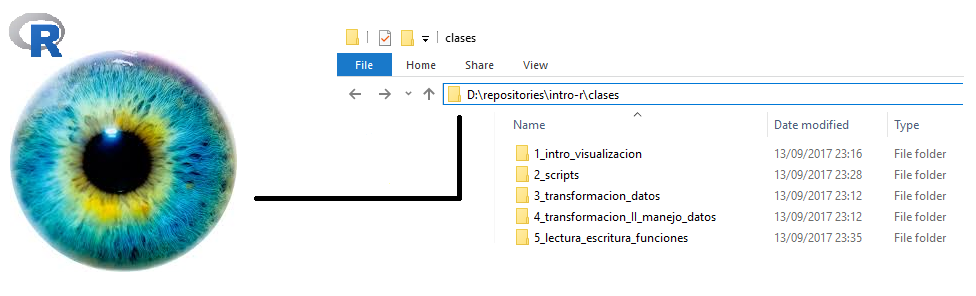
\includegraphics[width=13.56in]{./imagenes/1_ojo}

R puede ``ver'' lo que sea que le muestres, esto es, puedes decirle
exáctamente dónde debe buscar un archivo, por ejemplo indicando con una
cadena de texto una ruta completa en nuestro sistema de archivos (disco
duro):
``D:\textbackslash{}repositories\textbackslash{}intro-r\textbackslash{}''.
Estas rutas se pueden escribir manualmente, o se pueden copiar del
explorador de archivos de nuestro sistema operativo y luego pegarla en
R.


\includegraphics[width=9.01in]{./imagenes/2_ruta}

Es muy importante notar que en Windows, la convención es usar diagonales
invertidas ``\textbackslash{}'' para separar los niveles de nuestra
ruta. R no va a entender que algo es una ruta si está construída con
estos símbolos. Si se copia y pega una ruta desde nuestro explorador de
archivos en Windows, debemos cambiar las diagonales invertidas por
diagonales: ``D:/repositories/intro-r/''.

Otra posibilidad, también ya mencionada, es indicarle a R que ``vea''
una carpeta de trabajo. En este momento R está ``viendo'' la siguiente
carpeta:

\begin{Shaded}
\begin{Highlighting}[]
\KeywordTok{getwd}\NormalTok{()}
\end{Highlighting}
\end{Shaded}

\begin{verbatim}
## [1] "/Users/agutierrez/Documents/R/r"
\end{verbatim}

Estoy indica que R no necesita una ruta completa para leer cualquier
cosa incluída en la carpeta anterior. Únicamente el archivo. Para
cambiar la carpeta de trabajo se utiliza la funcón setwd() que como
argumento escencial recibe una ruta.

Se recomienda trabajar un proyecto dado en un carpeta que a su vez
contenga una carpeta que amacene los datos que se usen para ese proyecto
en particular. Por ejemplo una carpeta llamada ``datos'', así las rutas
a los archivos siempre pueden ser carpetas relativas. No importa si la
carpeta del proyecto se copia a otro equipo de cómputo, bastará con
hacer setwd() a la carpeta del proyecto para que todo el código
funcione.

Otra cosa que vale la pena mencionar es que RStudio incluye un
explorador de archivos, ahí se puede navegar en las carpetas de nuestra
computadora y con las opciones disponibles en el ícono de engrane se
puede también asignar la carpeta de trabajo.

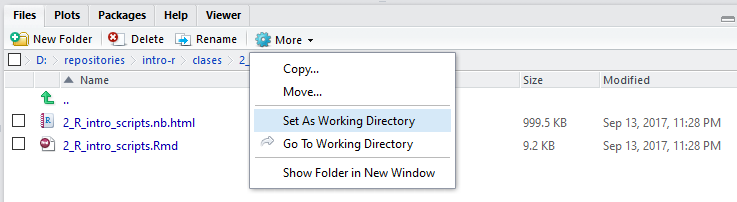
\includegraphics[width=10.24in]{./imagenes/3_setwd}

Es común que las tablas de datos se distribuyan como archivos de texto.
Existen numerosas variaciones de estos archivos de texto y csvs.

El tidyverse incluye al paquete readr que tiene como objetivo convertir
este tipo de archivos en data frames, aunque archivos de este tipo
delimitados por comas es lo más común, nos podemos encontrar con
archivos delimitados por otros símbolos, de aquí que existan las
siguiente funciones:

\begin{itemize}
\tightlist
\item
  read\_csv2() que lee archivos separados por punto y comas ``;''
\item
  read\_tsv() lee archivos separados por Tabs
\item
  read\_delim() lee archivos separados por cualquier símbolo (tú lo
  determinas con un argumento)
\item
  read\_fwf() lee archivos de anchos fijos, se pueden especificar los
  anchos con fwf\_widths() o su posición en el espacio (fila de datos)
  con fwf\_positions().
\item
  read\_table() lee un caso muy particular y popular de lo anterior que
  son archivos con datos separados por un único espacio.
\end{itemize}

Como ya se mencionó, todas estas funciones tienen una sintaxtis similar.
Lo más importante es alimentarles bien la ruta del archivo que se desea
leer.

Aunque este tipos de archivos son extremadamente populares en el mundo
de los archivos de datos, existen numerosas otras presentaciones. Por
ejemplo, es muy común el uso de Microsoft Excel para análisis
cuantitativo. R está bien preparado para leer y escribir archivos excel.

Bajaremos datos de Incidencia de Víctimas de homicidio, secuestro y
extorsión de datos.gob.mx:

\url{https://datos.gob.mx/busca/dataset/victimas-de-homicidio-secuestro-y-extorsion-excel}

Para leer estos datos se utilizaremos el paquete readxl (no se les
olvide instalarlo)

\begin{Shaded}
\begin{Highlighting}[]
\CommentTok{# cargar el paquete}
\KeywordTok{library}\NormalTok{(}\StringTok{"readxl"}\NormalTok{)}

\CommentTok{# ¿dónde está el archivo? recordar usar rutas relativas:}
\NormalTok{ruta_relativa <-}\StringTok{ "./datos/Estatal_Victimas_2015_2018_feb.xlsx"}

\CommentTok{# leer este archivo }
\NormalTok{datos <-}\StringTok{ }\KeywordTok{read_excel}\NormalTok{(ruta_relativa,}\DataTypeTok{sheet=}\DecValTok{1}\NormalTok{)}
\end{Highlighting}
\end{Shaded}

\subsection{2. Usar spread para transformar registros de un data frame
en
campos.}\label{usar-spread-para-transformar-registros-de-un-data-frame-en-campos.}

Al transformar registros en campos, se quitan renglones y se agregan
columnas, lo que se llama datos \textbf{anchos}.

Es importante notar que gather y spread son funciones inversas.

Primero veamos el estado original de la tabla de datos, tiene múltiples
columnas que corresponden a muchos cortes en la naturaleza de los
crímenes cometidos (Estado donde se comentió, mes cuando se comentió,
sexo de la víctima, tipo de crimen, etc).

\begin{Shaded}
\begin{Highlighting}[]
\CommentTok{# renombrar la primera variable porque incluye un molesto símbolo especial: ~}
\NormalTok{datos <-}\StringTok{ }\KeywordTok{rename}\NormalTok{(datos, }\DataTypeTok{Anio =}\NormalTok{ Año)}


\CommentTok{# generar totales por mes}
\NormalTok{datos <-}\StringTok{ }\NormalTok{datos }\OperatorTok\StringTok{ }
\StringTok{         }\KeywordTok{mutate}\NormalTok{(}\DataTypeTok{total =} \KeywordTok{select}\NormalTok{(.,Enero}\OperatorTok{:}\NormalTok{Diciembre) }\OperatorTok\StringTok{ }\KeywordTok{rowSums}\NormalTok{())}
\end{Highlighting}
\end{Shaded}

Ahora sí vamos a pasar la tabla de datos a un formato largo con base en
los tipos de delitos

\begin{Shaded}
\begin{Highlighting}[]
\CommentTok{# trabajar sólo Homicidios y Feminicidios, pasar a los datos a formato largo por año}

\CommentTok{# Usando la función spread para transformar registros en campos:}
\CommentTok{# key: variable cuyos valores definirán los nombres de nuestros campos. Para}
\CommentTok{# revertir el data frame usaremos "enfermedad"}

\NormalTok{tipos_delito =}\StringTok{ }\NormalTok{datos }\OperatorTok\StringTok{ }
\StringTok{                  }\KeywordTok{spread}\NormalTok{(}\DataTypeTok{key =} \StringTok{`}\DataTypeTok{Tipo de delito}\StringTok{`}\NormalTok{, }\DataTypeTok{value =}\NormalTok{ total)}
\end{Highlighting}
\end{Shaded}

Ya que está en formato largo, se puede generar una útil tabla de conteo
de delitos cruzado por Entidad, Año y Sexo.

\begin{Shaded}
\begin{Highlighting}[]
\CommentTok{# cantidad de subtipos de delito por entidad, año y sexo}
\NormalTok{cantidad_tipos <-}\StringTok{    }\NormalTok{tipos_delito }\OperatorTok\StringTok{ }
\StringTok{                     }\KeywordTok{group_by}\NormalTok{(Entidad,Anio,Sexo) }\OperatorTok
\StringTok{                     }\KeywordTok{summarise_at}\NormalTok{ (}\DataTypeTok{.vars=}\KeywordTok{vars}\NormalTok{(Aborto}\OperatorTok{:}\NormalTok{Secuestro),}\DataTypeTok{.funs=}\NormalTok{sum,}\DataTypeTok{na.rm=}\OtherTok{TRUE}\NormalTok{)}
\end{Highlighting}
\end{Shaded}

\subsection{3. Usar gather para transformar campos de un data frame en
registros}\label{usar-gather-para-transformar-campos-de-un-data-frame-en-registros}

Al transformar campos en registros, se quitan columnas y se agregan
renglones al data frame. Esto se llama datos \textbf{largos}.

Podemos usar esta operación para eliminar las columnas-delitos de la
tabla de datos anterior y agregarla a unas columnas de conteos por
delito (estructura: nombre delito, conteo)

\begin{Shaded}
\begin{Highlighting}[]
\CommentTok{# Usando la función gather para transformar campos en registros:}
\CommentTok{# key: nombre de la columna con los nombres de los campos (ahora registros)}
\CommentTok{# value: nombre de la columna con los valores de los campos (numero_pacientes)}
\CommentTok{# lo que sigue son las columnas que definen los campos que se transformarán en renglones}
\NormalTok{cantidad_tipos_largos <-}\StringTok{ }\KeywordTok{gather}\NormalTok{(cantidad_tipos, }
                                \DataTypeTok{key =} \StringTok{"tipo_delito"}\NormalTok{, }
                                \DataTypeTok{value =} \StringTok{"num_delitos_cometidos"}\NormalTok{,}
\NormalTok{                                Aborto}\OperatorTok{:}\NormalTok{Secuestro)}
\end{Highlighting}
\end{Shaded}


\includegraphics{./imagenes/manicule2.jpg} A partir de los datos
originales, crear otra tabla que sea interesante utilizando las
funciones gather o spread y las otras funciones de manipulación vistas
hasta ahora. Investigar el uso de la función de escritura de texto
delimitado write\_csv(), también del paquete reader, y utilizarla para
guardar la tabla de datos anterior a su carpeta ``datos''.

\subsection{4. Separar una columna en dos o más: separate(df, col =
columna, into = c(nueva\_variable\_1, nueva\_variable\_2,
etc)}\label{separar-una-columna-en-dos-o-mas-separatedf-col-columna-into-cnueva_variable_1-nueva_variable_2-etc}

Separate es una función útil para separar una columna de un data frame
en varias columnas, cuyos nombres se especifican. La separación default
se realiza por caracteres especiales (., \_, espacios, etc). Por
ejemplo:

\begin{Shaded}
\begin{Highlighting}[]
\NormalTok{instructores_curso_r <-}\StringTok{ }\KeywordTok{data_frame}\NormalTok{(}
  \DataTypeTok{id =} \KeywordTok{c}\NormalTok{(}\DecValTok{1}\NormalTok{,}\DecValTok{2}\NormalTok{,}\DecValTok{3}\NormalTok{),}
  \DataTypeTok{nombre =} \KeywordTok{c}\NormalTok{(}
    \StringTok{"Amaury Gutiérrez"}\NormalTok{,}
    \StringTok{"Teresa Ortiz"}\NormalTok{,}
    \StringTok{"Julian_Equihua"}
\NormalTok{  )}
\NormalTok{)}
\NormalTok{instructores_curso_r}
\end{Highlighting}
\end{Shaded}

\begin{verbatim}
## # A tibble: 3 x 2
##      id nombre          
##   <dbl> <chr>           
## 1     1 Amaury Gutiérrez
## 2     2 Teresa Ortiz    
## 3     3 Julian_Equihua
\end{verbatim}

\begin{Shaded}
\begin{Highlighting}[]
\KeywordTok{separate}\NormalTok{(instructores_curso_r, nombre, }\DataTypeTok{into =} \KeywordTok{c}\NormalTok{(}\StringTok{"nombre"}\NormalTok{, }\StringTok{"apellido_1"}\NormalTok{))}
\end{Highlighting}
\end{Shaded}

\begin{verbatim}
## # A tibble: 3 x 3
##      id nombre apellido_1
##   <dbl> <chr>  <chr>     
## 1     1 Amaury Gutiérrez 
## 2     2 Teresa Ortiz     
## 3     3 Julian Equihua
\end{verbatim}


\includegraphics{./imagenes/manicule2.jpg} Evalúa las siguientes
expresiones, y explica con tus palabras lo que sucede

\begin{Shaded}
\begin{Highlighting}[]
\NormalTok{instructores_curso_r_}\DecValTok{1}\NormalTok{ <-}\StringTok{ }\KeywordTok{data_frame}\NormalTok{(}
  \DataTypeTok{id =} \KeywordTok{c}\NormalTok{(}\DecValTok{1}\NormalTok{,}\DecValTok{2}\NormalTok{,}\DecValTok{3}\NormalTok{),}
  \DataTypeTok{nombre =} \KeywordTok{c}\NormalTok{(}
    \StringTok{"Fernando Pardo Urrutia"}\NormalTok{,}
    \StringTok{"Teresa Ortiz"}\NormalTok{,}
    \StringTok{"Julian_Equihua"}
\NormalTok{  )}
\NormalTok{)}

\KeywordTok{separate}\NormalTok{(instructores_curso_r_}\DecValTok{1}\NormalTok{, nombre, }\DataTypeTok{into =} \KeywordTok{c}\NormalTok{(}\StringTok{"nombre"}\NormalTok{, }\StringTok{"apellido_1"}\NormalTok{))}
\KeywordTok{separate}\NormalTok{(instructores_curso_r_}\DecValTok{1}\NormalTok{, nombre, }\DataTypeTok{into =} \KeywordTok{c}\NormalTok{(}\StringTok{"nombre"}\NormalTok{, }\StringTok{"apellido_1"}\NormalTok{, }\StringTok{"apellido_2"}\NormalTok{))}
\end{Highlighting}
\end{Shaded}


\includegraphics{./imagenes/manicule2.jpg} Da una explicación intuitiva
de lo que es el \textbf{NA}

\section{Datos faltantes}\label{datos-faltantes}

Un \textbf{NA} es un dato faltante, es decir, un vacío en una tabla.
Como en R los data frames contienen un elemento en cada campo, estos
vacíos se traducen como datos faltantes.

\textbf{Como son vacíos de información, los datos faltantes se pueden
pensar como ``no sé''}

\begin{Shaded}
\begin{Highlighting}[]
\OtherTok{NA} \CommentTok{# Dato Faltante}
\end{Highlighting}
\end{Shaded}

\begin{verbatim}
## [1] NA
\end{verbatim}

\begin{Shaded}
\begin{Highlighting}[]
\OtherTok{NA} \OperatorTok{+}\StringTok{ }\DecValTok{3} \CommentTok{# No se + 3 = No sé}
\end{Highlighting}
\end{Shaded}

\begin{verbatim}
## [1] NA
\end{verbatim}

\begin{Shaded}
\begin{Highlighting}[]
\OtherTok{NA} \OperatorTok{*}\StringTok{ }\DecValTok{3} \CommentTok{# No se * 3 = No sé}
\end{Highlighting}
\end{Shaded}

\begin{verbatim}
## [1] NA
\end{verbatim}

\begin{Shaded}
\begin{Highlighting}[]
\KeywordTok{is.na}\NormalTok{(}\OtherTok{NA}\NormalTok{) }\CommentTok{# Un operador binario para preguntar si un dato es faltante (NA)}
\end{Highlighting}
\end{Shaded}

\begin{verbatim}
## [1] TRUE
\end{verbatim}

\begin{Shaded}
\begin{Highlighting}[]
\KeywordTok{is.na}\NormalTok{(}\FloatTok{5.3}\NormalTok{)}
\end{Highlighting}
\end{Shaded}

\begin{verbatim}
## [1] FALSE
\end{verbatim}

\begin{Shaded}
\begin{Highlighting}[]
\KeywordTok{is.na}\NormalTok{(}\OtherTok{FALSE}\NormalTok{)}
\end{Highlighting}
\end{Shaded}

\begin{verbatim}
## [1] FALSE
\end{verbatim}

\begin{Shaded}
\begin{Highlighting}[]
\OtherTok{FALSE} \OperatorTok{|}\StringTok{ }\OtherTok{NA} \CommentTok{# No se cuánto da FALSE ó NA}
\end{Highlighting}
\end{Shaded}

\begin{verbatim}
## [1] NA
\end{verbatim}

\begin{Shaded}
\begin{Highlighting}[]
\OtherTok{TRUE} \OperatorTok{|}\StringTok{ }\OtherTok{NA} \CommentTok{# Pero TRUE o NA sí, porque sabemos que verdadero ó lo que sea ya es verdadero: como (5 > 3) | (1 > 3)}
\end{Highlighting}
\end{Shaded}

\begin{verbatim}
## [1] TRUE
\end{verbatim}

\begin{Shaded}
\begin{Highlighting}[]
\OtherTok{NA} \OperatorTok{>}\StringTok{ }\DecValTok{5} \CommentTok{# ¿Es NO SE > 5? NO Sé}
\end{Highlighting}
\end{Shaded}

\begin{verbatim}
## [1] NA
\end{verbatim}

\begin{Shaded}
\begin{Highlighting}[]
\OtherTok{NA} \OperatorTok{==}\StringTok{ }\OtherTok{NA} \CommentTok{#¿Es NO SE igual a NO SÉ? NO SÉ}
\end{Highlighting}
\end{Shaded}

\begin{verbatim}
## [1] NA
\end{verbatim}

\begin{Shaded}
\begin{Highlighting}[]
\KeywordTok{sum}\NormalTok{(}\KeywordTok{c}\NormalTok{(}\DecValTok{4}\NormalTok{, }\DecValTok{5}\NormalTok{, }\DecValTok{6}\NormalTok{, }\OtherTok{NA}\NormalTok{)) }\CommentTok{# No se cuanto da la suma de algo 4, 5, 6, y no sé.}
\end{Highlighting}
\end{Shaded}

\begin{verbatim}
## [1] NA
\end{verbatim}

\begin{Shaded}
\begin{Highlighting}[]
\KeywordTok{sum}\NormalTok{(}\KeywordTok{c}\NormalTok{(}\DecValTok{4}\NormalTok{, }\DecValTok{5}\NormalTok{, }\DecValTok{6}\NormalTok{, }\OtherTok{NA}\NormalTok{), }\DataTypeTok{na.rm =} \OtherTok{TRUE}\NormalTok{) }\CommentTok{# Pero puedo decirle a R que remueva los NA's}
\end{Highlighting}
\end{Shaded}

\begin{verbatim}
## [1] 15
\end{verbatim}

\begin{Shaded}
\begin{Highlighting}[]
\KeywordTok{mean}\NormalTok{(}\KeywordTok{c}\NormalTok{(}\DecValTok{4}\NormalTok{, }\DecValTok{5}\NormalTok{, }\DecValTok{6}\NormalTok{, }\OtherTok{NA}\NormalTok{), }\DataTypeTok{na.rm =} \OtherTok{TRUE}\NormalTok{)}
\end{Highlighting}
\end{Shaded}

\begin{verbatim}
## [1] 5
\end{verbatim}

\begin{Shaded}
\begin{Highlighting}[]
\CommentTok{# Dado un data frame con datos faltantes}
\NormalTok{registro <-}\StringTok{ }\KeywordTok{data_frame}\NormalTok{(}
  \DataTypeTok{id =} \KeywordTok{c}\NormalTok{(}\DecValTok{1}\NormalTok{, }\DecValTok{2}\NormalTok{, }\DecValTok{3}\NormalTok{),}
  \DataTypeTok{persona =} \KeywordTok{c}\NormalTok{(}\StringTok{"Fernando"}\NormalTok{, }\OtherTok{NA}\NormalTok{, }\StringTok{"Julián"}\NormalTok{),}
  \DataTypeTok{numero_socio =} \KeywordTok{c}\NormalTok{(}\DecValTok{13}\NormalTok{, }\DecValTok{12}\NormalTok{, }\OtherTok{NA}\NormalTok{)}
\NormalTok{)}
\NormalTok{registro}
\end{Highlighting}
\end{Shaded}

\begin{verbatim}
## # A tibble: 3 x 3
##      id persona  numero_socio
##   <dbl> <chr>           <dbl>
## 1     1 Fernando           13
## 2     2 <NA>               12
## 3     3 Julián             NA
\end{verbatim}

\begin{Shaded}
\begin{Highlighting}[]
\CommentTok{# Puedo seleccionar renglones con NA:}
\NormalTok{registro }\OperatorTok
\StringTok{  }\KeywordTok{filter}\NormalTok{(}\KeywordTok{is.na}\NormalTok{(persona))}
\end{Highlighting}
\end{Shaded}

\begin{verbatim}
## # A tibble: 1 x 3
##      id persona numero_socio
##   <dbl> <chr>          <dbl>
## 1     2 <NA>              12
\end{verbatim}

\begin{Shaded}
\begin{Highlighting}[]
\CommentTok{# O renglones sin NA:}
\NormalTok{registro }\OperatorTok
\StringTok{  }\KeywordTok{filter}\NormalTok{(}\OperatorTok{!}\KeywordTok{is.na}\NormalTok{(persona))}
\end{Highlighting}
\end{Shaded}

\begin{verbatim}
## # A tibble: 2 x 3
##      id persona  numero_socio
##   <dbl> <chr>           <dbl>
## 1     1 Fernando           13
## 2     3 Julián             NA
\end{verbatim}

\begin{Shaded}
\begin{Highlighting}[]
\CommentTok{# Puedo usar las reglas anteriores para calcular nuevas columnas:}
\NormalTok{registro }\OperatorTok
\StringTok{  }\KeywordTok{mutate}\NormalTok{(}\DataTypeTok{numero_socio_nuevo =}\NormalTok{ numero_socio }\OperatorTok{+}\StringTok{ }\DecValTok{1}\NormalTok{)}
\end{Highlighting}
\end{Shaded}

\begin{verbatim}
## # A tibble: 3 x 4
##      id persona  numero_socio numero_socio_nuevo
##   <dbl> <chr>           <dbl>              <dbl>
## 1     1 Fernando           13                 14
## 2     2 <NA>               12                 13
## 3     3 Julián             NA                 NA
\end{verbatim}

\begin{Shaded}
\begin{Highlighting}[]
\CommentTok{# Puedo ordenar y los NA's quedan al final}
\NormalTok{registro }\OperatorTok
\StringTok{  }\KeywordTok{arrange}\NormalTok{(numero_socio)}
\end{Highlighting}
\end{Shaded}

\begin{verbatim}
## # A tibble: 3 x 3
##      id persona  numero_socio
##   <dbl> <chr>           <dbl>
## 1     2 <NA>               12
## 2     1 Fernando           13
## 3     3 Julián             NA
\end{verbatim}

\begin{Shaded}
\begin{Highlighting}[]
\CommentTok{# Puedo ordenar y los NA's quedan al final}
\NormalTok{registro }\OperatorTok
\StringTok{  }\KeywordTok{arrange}\NormalTok{(}\KeywordTok{desc}\NormalTok{(numero_socio))}
\end{Highlighting}
\end{Shaded}

\begin{verbatim}
## # A tibble: 3 x 3
##      id persona  numero_socio
##   <dbl> <chr>           <dbl>
## 1     1 Fernando           13
## 2     2 <NA>               12
## 3     3 Julián             NA
\end{verbatim}

\begin{Shaded}
\begin{Highlighting}[]
\CommentTok{# Tengo que tener cuidado con calcular resúmenes de data frames que contienen NA's}
\NormalTok{registro }\OperatorTok
\StringTok{  }\KeywordTok{summarise}\NormalTok{(}\DataTypeTok{promedio =} \KeywordTok{mean}\NormalTok{(numero_socio))}
\end{Highlighting}
\end{Shaded}

\begin{verbatim}
## # A tibble: 1 x 1
##   promedio
##      <dbl>
## 1       NA
\end{verbatim}

\begin{Shaded}
\begin{Highlighting}[]
\CommentTok{# Pero puedo arreglarlo fácilmente}
\NormalTok{registro }\OperatorTok
\StringTok{  }\KeywordTok{summarise}\NormalTok{(}\DataTypeTok{promedio =} \KeywordTok{mean}\NormalTok{(numero_socio, }\DataTypeTok{na.rm =} \OtherTok{TRUE}\NormalTok{))}
\end{Highlighting}
\end{Shaded}

\begin{verbatim}
## # A tibble: 1 x 1
##   promedio
##      <dbl>
## 1     12.5
\end{verbatim}


\includegraphics{./imagenes/manicule.jpg} Entregar un script donde se
lleve a cabo un proceso de manipulación y transformación de datos sobre
la tabla de delitos. Adicionalmente generar un gráfico interesante
utilizando lo visto en las clases de visualización de datos. Comentar
cada paso y explicar qué comunica la gráfica generada.

\chapter{Funciones}\label{funciones}

\section{¿Qué aprendimos la clase
pasada?}\label{que-aprendimos-la-clase-pasada-2}

\begin{itemize}
\tightlist
\item
  Se aprendió a usar el operador pipe \%\textgreater{}\%
\item
  Se mostró el concepto de hacer joins entre tablas
\item
  Lectura de datos en R (excel)
\item
  Breve introdución a los datos faltantes
\end{itemize}

\section{Funciones en R}\label{funciones-en-r-1}

Las funciones permiten la automatización de tareas. La escritura de
funciones tiene tres grandes ventajas:

\begin{itemize}
\tightlist
\item
  Puedes nombrar una función de una manera tal que nunca olvides qué
  hace, esto además hace a tu código más legible
\item
  Cuando cambien los requerimientos de los trabajos día a día, deberás
  de modificar menos código.
\item
  Se reduce la probabilidad de cometer errores llevando a cabo procesos
  manuales como copiar/pegar datos e instrucciones.
\end{itemize}

Aprender a escrbir buenas funciones es un proceso que nunca termina.
Siempre se encontrarán maneras novedosas de mejorar estilos a la hora de
escribir funciones. Esta sección no tiene como objetivo profundizar en
la escritura de funciones, si no empezar a escribir funciones útiles lo
más pronto posible.

\subsection{¿Cuándo es conveniente escribir
funciones?}\label{cuando-es-conveniente-escribir-funciones}

Como regla general, si notamos que para llevar a cabo una cierta tarea
se está copiando y pegando un bloque de código más de dos veces, es hora
de escribir una función para ello. Motivaremos la discusión con el
cálculo de areas y volúmenes. Si escribimos una función en R que permita
llevar a cabo estas operaciones, las podremos usar en cualquier momento.

\begin{figure}
\centering
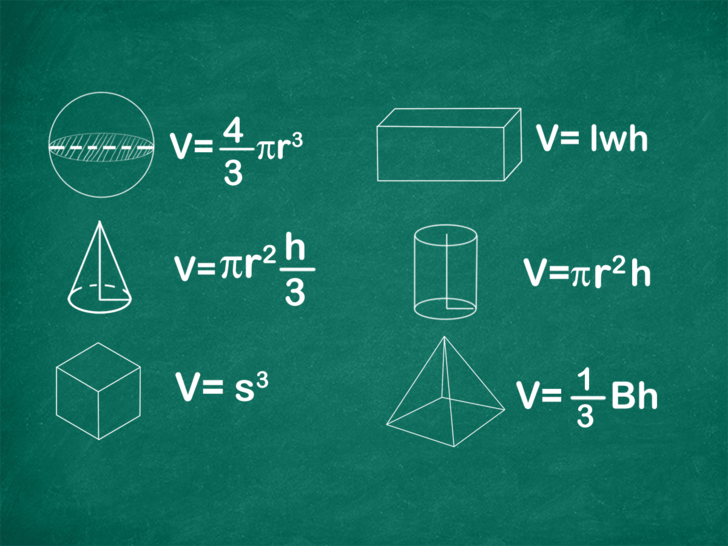
\includegraphics{./imagenes/volume.png}
\caption{}
\end{figure}

\subsection{Escribiendo funciones en
R}\label{escribiendo-funciones-en-r}

Pasos para crear una función:

\begin{itemize}
\tightlist
\item
  Elegir un nombre apropiado
\item
  Pensar en qué hace y cuántos argumentos necesita para ejecutarse
\item
  Traducir lo que queremos que haga a código de R dentro de un bloque
  asociado a una función y a los argumentos anteriores
\end{itemize}

Pensando en estos pasos decidamos que nuestra función se llame
area\_circulo() (sin acento, es en general, mala práctica utilizar
caractéres especiales en código). Luego sabemos que la función recibe un
único parámetro, el radio del círculo al que se le va a calcular el
área. Finalmente se debe plasmar la fórmula para el cálculo del área de
un círculo en R.

Como un primer ejemplo escribamos una función que permita calcular el
área de un círculo.

\begin{Shaded}
\begin{Highlighting}[]
\CommentTok{# nombre ------------- argumentos}
\NormalTok{area_circulo <-}\StringTok{ }\ControlFlowTok{function}\NormalTok{ (radio) \{}
  \ControlFlowTok{if}\NormalTok{ (radio }\OperatorTok{<}\StringTok{ }\DecValTok{0}\NormalTok{) }\CommentTok{# expresión condicional se ejecuta en caso de que el radio sea negativo.}
\NormalTok{  \{}
    \KeywordTok{stop}\NormalTok{(}\StringTok{"Para calcular un area es necesario un valor positivo o igual a 0."}\NormalTok{) }\CommentTok{# detiene la ejecución}
\NormalTok{  \} }\ControlFlowTok{else} \CommentTok{# sigue la expresión condicional, este bloque se ejecutará cuando el radio sea positivo.}
\NormalTok{  \{}
\NormalTok{    area_calculada <-}\StringTok{ }\NormalTok{pi }\OperatorTok{*}\StringTok{ }\NormalTok{radio }\OperatorTok{**}\StringTok{ }\DecValTok{2} \CommentTok{# operamos sobre el radio del círculo}
    \KeywordTok{return}\NormalTok{(area_calculada) }\CommentTok{# regresamos el resultado (se asigna después de aplicar esta función)}
\NormalTok{  \}}
  
\NormalTok{\}}
\end{Highlighting}
\end{Shaded}

Para probar la función la llamamos como cualquier función de una
libreria, notemos que es posible asignar el resultado a una variable:

\begin{Shaded}
\begin{Highlighting}[]
\NormalTok{area_radio_cinco <-}\StringTok{ }\KeywordTok{area_circulo}\NormalTok{(}\DecValTok{5}\NormalTok{)}
\NormalTok{area_radio_cinco}
\end{Highlighting}
\end{Shaded}

\begin{verbatim}
## [1] 78.53982
\end{verbatim}


\includegraphics{./imagenes/manicule2.jpg} Ejercicio 1: Escribir una
función análoga a la anterior pero para calcular el área de un
rectángulo.


\includegraphics{./imagenes/manicule2.jpg} Ejercicio 2: ¿Como podría
usar la función del ejercicio 1 para calcular el area de un cuadrado?

\subsection{Expresiones condicionales}\label{expresiones-condicionales}

En ocasiones es deseable ejecutar bloques de código únicamente cuando
cierta condición se cumple. Existe una sentencia que nos permite hacer
esto y tiene la forma siguiente:

\begin{Shaded}
\begin{Highlighting}[]
\ControlFlowTok{if}\NormalTok{ (cond) \{}
  \CommentTok{# código ejecutado en caso de que la condición sea verdadera (TRUE).}
\NormalTok{\} }\ControlFlowTok{else}\NormalTok{ \{}
  \CommentTok{# código ejecutado en caso de que la condición sea falsa (FALSE).}
\NormalTok{\}}
\end{Highlighting}
\end{Shaded}

Es posible omitir la segunda condición:

\begin{Shaded}
\begin{Highlighting}[]
\ControlFlowTok{if}\NormalTok{ (cond) \{}
  \CommentTok{# si la condición es verdadera se ejecutará este bloque, en caso contrario no hará nada.}
\NormalTok{\}}
\end{Highlighting}
\end{Shaded}

También es posible encadenar sentencias condicionales:

\begin{Shaded}
\begin{Highlighting}[]
\ControlFlowTok{if}\NormalTok{ (cond_}\DecValTok{1}\NormalTok{) \{}
  \CommentTok{# código ejecutado en caso de que la condición 1 sea verdadera.}
\NormalTok{\} }\ControlFlowTok{else} \ControlFlowTok{if}\NormalTok{ (cond_}\DecValTok{2}\NormalTok{) \{}
  \CommentTok{# código ejecutado en caso de que la condición 1 sea falsa pero la condición 2 es verdadera.}
\NormalTok{\} }\ControlFlowTok{else}\NormalTok{ \{}
  \CommentTok{# cuando ambas condiciones son falsas se ejecuta este bloque.}
\NormalTok{\}}
\end{Highlighting}
\end{Shaded}

Regresando a nuestra función \emph{area\_circulo}, notemos que nuestra
formulación tiene un problema. ¿Qué pasa cuando la función recibe
números negativos? ¿Tiene sentido hablar de areas negativas? Usaremos
las sentencias condicionales para arreglar este detalle:

\begin{Shaded}
\begin{Highlighting}[]
\CommentTok{# nombre ------------- argumentos}
\NormalTok{area_circulo <-}\StringTok{ }\ControlFlowTok{function}\NormalTok{ (radio) \{}
  \ControlFlowTok{if}\NormalTok{ (radio }\OperatorTok{<}\StringTok{ }\DecValTok{0}\NormalTok{) }\CommentTok{# expresión condicional se ejecuta en caso de que el radio sea negativo.}
\NormalTok{  \{}
    \KeywordTok{stop}\NormalTok{(}\StringTok{"Para calcular un area es necesario un valor positivo o igual a 0."}\NormalTok{) }\CommentTok{# detiene la ejecución}
\NormalTok{  \} }\ControlFlowTok{else} \CommentTok{# sigue la expresión condicional, este bloque se ejecutará cuando el radio sea positivo.}
\NormalTok{  \{}
\NormalTok{    area_calculada <-}\StringTok{ }\NormalTok{pi }\OperatorTok{*}\StringTok{ }\NormalTok{radio}\OperatorTok{^}\DecValTok{2} \CommentTok{# operamos sobre el radio del círculo}
    \KeywordTok{return}\NormalTok{(area_calculada) }\CommentTok{# regresamos el resultado (se asigna después de aplicar esta función)}
\NormalTok{  \}}
  
\NormalTok{\}}
\end{Highlighting}
\end{Shaded}

Probemos nuestra función mejorada con ambos tipos de valores. ¿Qué pasa
cuando la usamos con un número negativo?

\begin{Shaded}
\begin{Highlighting}[]
\CommentTok{# probemos nuestra función en}
\NormalTok{area_resultante <-}\StringTok{ }\KeywordTok{area_circulo}\NormalTok{(}\OperatorTok{-}\DecValTok{10}\NormalTok{)}
\end{Highlighting}
\end{Shaded}

\begin{Shaded}
\begin{Highlighting}[]
\CommentTok{# probemos nuestra función en}
\NormalTok{area_resultante <-}\StringTok{ }\KeywordTok{area_circulo}\NormalTok{(}\DecValTok{7}\NormalTok{)}
\end{Highlighting}
\end{Shaded}


\includegraphics{./imagenes/manicule2.jpg} Ejercicio 3: Reescribir la
función que calcula el área de un rectángulo para solventar el error
permitir parámetros negativos.


\includegraphics{./imagenes/manicule2.jpg} Ejercicio 4: Escribir una
función llamada salario que reciba un número que representara el salario
de un empleado. Si el salario es mayor a 25,000 deberá regresar el texto
``alto'', si el salario es menor a 5000 regresará ``bajo'', en otro caso
regresará ``medio''. Si recibe un salario negativo la función debera
detenerse y lanzar un mensaje de error.

\subsection{De regreso al tidyverse}\label{de-regreso-al-tidyverse}

\begin{figure}
\centering

\includegraphics{./imagenes/ceci.jpg}
\caption{}
\end{figure}

Para conectar con lo visto en clases pasadas veremos que es posible
encadenar nuestras funciones con el método de los pipes. Para
ejemplificar esto regresaremos a nuestro objetivo inicial, el cálculo de
volúmenes. Recordemos que los volúmenes de figuras regulares se pueden
calcular multiplicando el area de la base del objeto por su altura,
nuestra función queda definida de la siguiente forma:

\begin{Shaded}
\begin{Highlighting}[]
\NormalTok{volumen_regular <-}\StringTok{ }\ControlFlowTok{function}\NormalTok{ (area_base, altura) \{}
  \ControlFlowTok{if}\NormalTok{ (area_base }\OperatorTok{<}\StringTok{ }\DecValTok{0} \OperatorTok{||}\StringTok{ }\NormalTok{altura }\OperatorTok{<}\StringTok{ }\DecValTok{0}\NormalTok{) \{ }\CommentTok{# nos aseguramos que ninguno de los argumentos sea negativo.}
    \KeywordTok{stop}\NormalTok{(}\StringTok{"Tanto el area como la altura deben ser mayores o iguales a 0."}\NormalTok{)}
\NormalTok{  \} }\ControlFlowTok{else}\NormalTok{ \{}
\NormalTok{    volumen <-}\StringTok{ }\NormalTok{area_base }\OperatorTok{*}\StringTok{ }\NormalTok{altura}
    \KeywordTok{return}\NormalTok{(volumen)}
\NormalTok{  \}}
\NormalTok{\}}
\end{Highlighting}
\end{Shaded}

Podemos calcular el volumen de un cilindro de area 3 y altura 7 de la
siguiente forma:

\begin{Shaded}
\begin{Highlighting}[]
\CommentTok{# definimos las dimensiones}
\NormalTok{radio <-}\StringTok{ }\DecValTok{3}
\NormalTok{altura <-}\StringTok{ }\DecValTok{7}
\CommentTok{# calculamos área y volumen }
\NormalTok{area_base <-}\StringTok{ }\KeywordTok{area_circulo}\NormalTok{(radio)}
\NormalTok{volumen_cilindro <-}\StringTok{ }\KeywordTok{volumen_regular}\NormalTok{(area_base, altura)}
\CommentTok{#imprimimos el resultado}
\NormalTok{volumen_cilindro}
\end{Highlighting}
\end{Shaded}

\begin{verbatim}
## [1] 197.9203
\end{verbatim}

En una sola sentencia:

\begin{Shaded}
\begin{Highlighting}[]
\NormalTok{volumen_cilindro <-}\StringTok{ }\KeywordTok{volumen_regular}\NormalTok{(}\KeywordTok{area_circulo}\NormalTok{(}\DecValTok{3}\NormalTok{), }\DecValTok{7}\NormalTok{)}
\CommentTok{#imprimimos el resultado}
\NormalTok{volumen_cilindro}
\end{Highlighting}
\end{Shaded}

\begin{verbatim}
## [1] 197.9203
\end{verbatim}

Sin embargo nada impide hacer el uso del flujo que implementan los
pipes. De este modo es posible hacer que el código sea más legible al
encadenar las operaciones de izquierda a derecha en vez de adentro hacia
afuera:

\begin{Shaded}
\begin{Highlighting}[]
\KeywordTok{library}\NormalTok{(tidyverse)}
\NormalTok{volumen_cilindro <-}\StringTok{ }\DecValTok{3} \OperatorTok
\StringTok{                      }\NormalTok{area_circulo }\OperatorTok
\StringTok{                      }\KeywordTok{volumen_regular}\NormalTok{(}\DecValTok{7}\NormalTok{)}
\NormalTok{volumen_cilindro}
\end{Highlighting}
\end{Shaded}

\begin{verbatim}
## [1] 197.9203
\end{verbatim}

Nota: Recordemos que al usar los pipes, el resultado de una función en
la cadena será el argumento de la siguiente. En caso de que la siguiente
función requiera más de un argumento el resultado de la función se usará
como el primer argumento y resto se tienen que especificar
explícitamente.


\includegraphics{./imagenes/manicule2.jpg} Ejercicio 5: Reusa este
procedimiento para calcular el volumen de un cubo de lado 6 y un
paralelepípedo de dimensiones 4, 5 y 7.

\subsection{Ambientes}\label{ambientes}

Otro componente de las funciones es el ambiente. Hasta ahora no ha sido
mencionado porque hemos sido muy correctos en la definición de nuestras
funciones. Cada variable dentro de la función ha sido pasada como un
argumento o bien definida dentro de la función. ¿Qué pasaria si usaramos
una variable que no ha sido definida dentro del cuerpo de la función ni
ha sido pasada como argumento? Resulta que R es laxo con este tipo de
situaciones y lo que hace es buscar si la variable ha sido definida en
el contexto en el que se definió la función:

\begin{Shaded}
\begin{Highlighting}[]
\NormalTok{y <-}\StringTok{ }\DecValTok{19}

\NormalTok{suma_incorrecta <-}\StringTok{ }\ControlFlowTok{function}\NormalTok{(x) \{}
  \KeywordTok{return}\NormalTok{(x }\OperatorTok{+}\StringTok{ }\NormalTok{y)}
\NormalTok{\}}

\KeywordTok{suma_incorrecta}\NormalTok{(}\DecValTok{6}\NormalTok{)}
\end{Highlighting}
\end{Shaded}

\begin{verbatim}
## [1] 25
\end{verbatim}

Esto no es recomendable ya que el valor de \emph{y} puede perderse
cuando se vuelva a reiniciar RStudio. Este tipo de código puede
introducir errores difíciles de rastrear.

\subsection{Estilos de código y buenas
prácticas}\label{estilos-de-codigo-y-buenas-practicas}

Existen diversos estilos de programación, especialmente en R. Ninguno de
estos estilos es correcto, pero la consistencia permite que leer y
mantener el código sea más sencillo. Para nombrar variables y funciones
existen varias convenciones:

\begin{verbatim}
este_se_llama_snake_case
losProgramadoresSuelenUsarCamelCase
a.mi.no.me.gusta.usar.puntos
Some.menJust_WantTO.Watch.theWorld_BURN
\end{verbatim}

Como han podido darse cuenta nosotros usamos snake case.

Cuando los statements condicionales son de una sola sentencia es posible
no usar las llaves \{ \}. Sin embargo esto reduce la legilibidad del
código.

\begin{Shaded}
\begin{Highlighting}[]
\CommentTok{# BIEN las llaves permiten identificar que el código será ejecutado cuando la condición se cumple}
\NormalTok{muestra_mensaje <-}\StringTok{ }\OtherTok{TRUE}
\ControlFlowTok{if}\NormalTok{ (y }\OperatorTok{<}\StringTok{ }\DecValTok{0} \OperatorTok{&&}\StringTok{ }\NormalTok{muestra_mensaje) \{}
  \KeywordTok{message}\NormalTok{(}\StringTok{"y es negativo"}\NormalTok{)}
\NormalTok{\}}

\CommentTok{# MAL no hay jerarquía visual}
\NormalTok{muestra_mensaje <-}\StringTok{ }\OtherTok{TRUE}
\ControlFlowTok{if}\NormalTok{ (y }\OperatorTok{<}\StringTok{ }\DecValTok{0} \OperatorTok{&&}\StringTok{ }\NormalTok{muestra_mensaje)}
\KeywordTok{message}\NormalTok{(}\StringTok{"y es negativo"}\NormalTok{)}
\end{Highlighting}
\end{Shaded}

Ahora que saben que se puede hacer\ldots{} ¡No lo hagan!

La elección de nombres es un tema importante a considerar. El código es
un vínculo entre las instrucciones que una computadora puede ejecutar y
la forma en la que nosotros resolvemos un problema. El lenguaje de
programación nos permite expresar la serie de pasos necesarios para
llegar a una solución. Por esto el lenguaje debe no solo ejecutarse
correctamente sino también legible para el ojo humano. Los nombres en
las variables nos pueden ayudar a esto. Revisemos los nombres de
nuestras funciones de área:

\begin{Shaded}
\begin{Highlighting}[]
\CommentTok{# BIEN la ayuda de r aparece cuando escribo area y me permite recordar que nombre asigné a cada función}
\KeywordTok{area_circulo}\NormalTok{(}\DecValTok{4}\NormalTok{)}
\KeywordTok{area_cuadrado}\NormalTok{(}\DecValTok{3}\NormalTok{)}
\KeywordTok{area_rectangulo}\NormalTok{(}\DecValTok{5}\NormalTok{,}\DecValTok{6}\NormalTok{)}

\CommentTok{# MAL}
\KeywordTok{circulo_area}\NormalTok{(}\DecValTok{4}\NormalTok{) }\CommentTok{# el elemento en comun de las funciones no está al principio, dificulta la búsqueda}
\KeywordTok{calcula_area_cuadrado}\NormalTok{(}\DecValTok{3}\NormalTok{) }\CommentTok{# nomrbe demasiado largo, el verbo sobra porque está implícito}
\KeywordTok{mi_funcion}\NormalTok{(}\DecValTok{5}\NormalTok{,}\DecValTok{6}\NormalTok{) }\CommentTok{# todo mal, ¡no tenemos idea que hace la función!}
\end{Highlighting}
\end{Shaded}

Repitiendo lo que se menciona al principio de la sección no hay una
forma correcta de escribir código (existen muchas incorrectas), pero lo
más importante es \textbf{ser consistente}.

\subsection{Temas avanzados de funciones
(OPCIONAL)}\label{temas-avanzados-de-funciones-opcional}

Esta sección solo es demostrativa de las cosas que permite el lenguaje R
sobre las funciones. Se mencionan para hacer más amplio el repertorio en
caso de que alguien se interese en indagar más al respecto.

\subsubsection{Funciones recursivas}\label{funciones-recursivas}

\section{\texorpdfstring{\emph{Las funciones pueden llamarse a si
mismas.}}{Las funciones pueden llamarse a si mismas.}}\label{las-funciones-pueden-llamarse-a-si-mismas.}

\begin{figure}
\centering

\includegraphics{./imagenes/fear.png}
\caption{}
\end{figure}

¿Para que querríamos algo así? Las funciones recursivas permiten
calcular problemas cuya repesentación se puede formular en terminos de
si mismas. El ejemplo por excelencia es la operación factorial:

\[
n!=n\times(n-1)\times(n-2)\times\ldots\times2\times1
\]

Notemos que:

\[
n!=n\times(n-1)!
\] Y a su vez es:

\[
n!=n\times(n-1)\times(n-2)!
\]

Y sí sucesivamente hasta que llegamos hasta el \(1\).

Por lo que podemos definir una función que calcule dicha operación
haciendo uso de la misma definición:

\begin{Shaded}
\begin{Highlighting}[]
\NormalTok{factorial <-}\StringTok{ }\ControlFlowTok{function}\NormalTok{ (n) \{}
  \ControlFlowTok{if}\NormalTok{(n }\OperatorTok{==}\StringTok{ }\DecValTok{1}\NormalTok{) \{}
    \KeywordTok{return}\NormalTok{(}\DecValTok{1}\NormalTok{) }\CommentTok{# caso base, no hace falta calcular más}
\NormalTok{  \} }\ControlFlowTok{else}\NormalTok{\{}
    \KeywordTok{return}\NormalTok{(n }\OperatorTok{*}\StringTok{ }\KeywordTok{factorial}\NormalTok{(n }\OperatorTok{-}\StringTok{ }\DecValTok{1}\NormalTok{)) }\CommentTok{# multiplico el número actual y calculo el factorial del número menos una unidad}
\NormalTok{  \}}
\NormalTok{\}}

\KeywordTok{factorial}\NormalTok{(}\DecValTok{5}\NormalTok{)}
\end{Highlighting}
\end{Shaded}

\begin{verbatim}
## [1] 120
\end{verbatim}

\subsubsection{Funciones de orden alto}\label{funciones-de-orden-alto}

\section{\texorpdfstring{\emph{Las funciones pueden regresar
funciones}:}{Las funciones pueden regresar funciones:}}\label{las-funciones-pueden-regresar-funciones}

\begin{figure}
\centering

\includegraphics{./imagenes/mind.png}
\caption{}
\end{figure}

R es un lenguaje en el que las funciones son objetos que se pueden
operar como los números, las cadenas de texto, los data frames.

Con lo que hemos aprendido es posible crear una funcion que permita
calcular el cuadrado de un número con ayuda del operador **:

\begin{Shaded}
\begin{Highlighting}[]
\NormalTok{cuadrado <-}\StringTok{ }\ControlFlowTok{function}\NormalTok{ (x) \{}
  \KeywordTok{return}\NormalTok{(x }\OperatorTok{**}\StringTok{ }\DecValTok{2}\NormalTok{)}
\NormalTok{\}}

\KeywordTok{cuadrado}\NormalTok{(}\DecValTok{4}\NormalTok{)}
\end{Highlighting}
\end{Shaded}

\begin{verbatim}
## [1] 16
\end{verbatim}

De la misma forma podemos obtener una función que calcule el cubo de un
número:

\begin{Shaded}
\begin{Highlighting}[]
\NormalTok{cubo <-}\StringTok{ }\ControlFlowTok{function}\NormalTok{ (x) \{}
  \KeywordTok{return}\NormalTok{(x }\OperatorTok{**}\StringTok{ }\DecValTok{3}\NormalTok{)}
\NormalTok{\}}

\KeywordTok{cubo}\NormalTok{(}\DecValTok{4}\NormalTok{)}
\end{Highlighting}
\end{Shaded}

\begin{verbatim}
## [1] 64
\end{verbatim}

Pero la estructura es básicamente la misma. ¿Es indispensable repetir el
mismo código cuando el patrón es tan claro? Resulta que R nos permite
hacer plantillas para este tipo de casos:

\begin{Shaded}
\begin{Highlighting}[]
\NormalTok{fabrica_potencia <-}\StringTok{ }\ControlFlowTok{function}\NormalTok{ (n) \{}
  \ControlFlowTok{function}\NormalTok{(x) \{}
    \KeywordTok{return}\NormalTok{(x }\OperatorTok{**}\StringTok{ }\NormalTok{n)}
\NormalTok{  \}}
\NormalTok{\}}
\end{Highlighting}
\end{Shaded}

Probemos el resultado:

\begin{Shaded}
\begin{Highlighting}[]
\NormalTok{cuadrado <-}\StringTok{ }\KeywordTok{fabrica_potencia}\NormalTok{(}\DecValTok{2}\NormalTok{)}
\KeywordTok{cuadrado}\NormalTok{(}\DecValTok{4}\NormalTok{)}
\end{Highlighting}
\end{Shaded}

\begin{verbatim}
## [1] 16
\end{verbatim}

\begin{Shaded}
\begin{Highlighting}[]
\NormalTok{cubo <-}\StringTok{ }\KeywordTok{fabrica_potencia}\NormalTok{(}\DecValTok{3}\NormalTok{)}
\KeywordTok{cubo}\NormalTok{(}\DecValTok{4}\NormalTok{)}
\end{Highlighting}
\end{Shaded}

\begin{verbatim}
## [1] 64
\end{verbatim}

\begin{Shaded}
\begin{Highlighting}[]
\NormalTok{potencia_doce <-}\StringTok{ }\KeywordTok{fabrica_potencia}\NormalTok{(}\DecValTok{12}\NormalTok{)}
\KeywordTok{potencia_doce}\NormalTok{(}\DecValTok{4}\NormalTok{)}
\end{Highlighting}
\end{Shaded}

\begin{verbatim}
## [1] 16777216
\end{verbatim}

\chapter{Vectores}\label{vectores}

\section{¿Qué aprendimos la clase
pasada?}\label{que-aprendimos-la-clase-pasada-3}

\begin{itemize}
\tightlist
\item
  Evitar repeticiones de código por medio de funciones
\item
  Ejecutar bloques de código usando una condición de control
\item
  Como usar funciones creadas por nosotros en conjunto con las
  herramientas del tidyverse
\item
  Buenas prácticas para la escritura de código y por qué es deseable el
  código limpio
\end{itemize}

\section{Vectores, listas y arreglos}\label{vectores-listas-y-arreglos}

Existen dos tipos de vectores en R:

\begin{itemize}
\tightlist
\item
  Los vectores atómicos, que son homogeneos, es decir contienen el mismo
  tipo de dato en cada una de sus entradas.
\item
  Las listas, que son heterogeneas, es decir pueden contener distintos
  tipos de datos en cada entrada incluso otras listas.
\end{itemize}

Los vectores atómicos pueden ser de 6 distintos tipos: \emph{logical},
\emph{integer}, \emph{double}, \emph{character}, \emph{complex}, y
\emph{raw}.

\begin{Shaded}
\begin{Highlighting}[]
\NormalTok{vector_logico <-}\StringTok{ }\KeywordTok{c}\NormalTok{(}\OtherTok{TRUE}\NormalTok{, }\OtherTok{FALSE}\NormalTok{, }\OtherTok{FALSE}\NormalTok{, }\OtherTok{TRUE}\NormalTok{)}
\NormalTok{vector_logico}
\end{Highlighting}
\end{Shaded}

\begin{verbatim}
## [1]  TRUE FALSE FALSE  TRUE
\end{verbatim}

\begin{Shaded}
\begin{Highlighting}[]
\KeywordTok{typeof}\NormalTok{(vector_logico)}
\end{Highlighting}
\end{Shaded}

\begin{verbatim}
## [1] "logical"
\end{verbatim}

\begin{Shaded}
\begin{Highlighting}[]
\NormalTok{vector_entero <-}\StringTok{ }\DecValTok{1}\OperatorTok{:}\DecValTok{4}
\NormalTok{vector_entero}
\end{Highlighting}
\end{Shaded}

\begin{verbatim}
## [1] 1 2 3 4
\end{verbatim}

\begin{Shaded}
\begin{Highlighting}[]
\KeywordTok{typeof}\NormalTok{(vector_entero)}
\end{Highlighting}
\end{Shaded}

\begin{verbatim}
## [1] "integer"
\end{verbatim}

\begin{Shaded}
\begin{Highlighting}[]
\NormalTok{vector_double <-}\StringTok{ }\KeywordTok{c}\NormalTok{(}\FloatTok{1.2}\NormalTok{, pi, }\KeywordTok{sqrt}\NormalTok{(}\DecValTok{3}\NormalTok{)) }
\NormalTok{vector_double}
\end{Highlighting}
\end{Shaded}

\begin{verbatim}
## [1] 1.200000 3.141593 1.732051
\end{verbatim}

\begin{Shaded}
\begin{Highlighting}[]
\KeywordTok{typeof}\NormalTok{(vector_double)}
\end{Highlighting}
\end{Shaded}

\begin{verbatim}
## [1] "double"
\end{verbatim}

\begin{Shaded}
\begin{Highlighting}[]
\NormalTok{vector_char <-}\StringTok{ }\NormalTok{letters[}\DecValTok{1}\OperatorTok{:}\DecValTok{4}\NormalTok{]}
\NormalTok{vector_char}
\end{Highlighting}
\end{Shaded}

\begin{verbatim}
## [1] "a" "b" "c" "d"
\end{verbatim}

\begin{Shaded}
\begin{Highlighting}[]
\KeywordTok{typeof}\NormalTok{(vector_char)}
\end{Highlighting}
\end{Shaded}

\begin{verbatim}
## [1] "character"
\end{verbatim}

\begin{Shaded}
\begin{Highlighting}[]
\NormalTok{vector_complex <-}\StringTok{ }\KeywordTok{c}\NormalTok{(}\DecValTok{1} \OperatorTok{+}\StringTok{ }\NormalTok{1i, 5i, }\DecValTok{5}\NormalTok{)}
\NormalTok{vector_complex}
\end{Highlighting}
\end{Shaded}

\begin{verbatim}
## [1] 1+1i 0+5i 5+0i
\end{verbatim}

\begin{Shaded}
\begin{Highlighting}[]
\KeywordTok{typeof}\NormalTok{(vector_complex)}
\end{Highlighting}
\end{Shaded}

\begin{verbatim}
## [1] "complex"
\end{verbatim}

\begin{Shaded}
\begin{Highlighting}[]
\NormalTok{vector_raw <-}\StringTok{ }\KeywordTok{c}\NormalTok{(}\KeywordTok{charToRaw}\NormalTok{(}\StringTok{"the quick brown fox jumps over the lazy dog"}\NormalTok{))}
\NormalTok{vector_raw}
\end{Highlighting}
\end{Shaded}

\begin{verbatim}
##  [1] 74 68 65 20 71 75 69 63 6b 20 62 72 6f 77 6e 20 66 6f 78 20 6a 75 6d
## [24] 70 73 20 6f 76 65 72 20 74 68 65 20 6c 61 7a 79 20 64 6f 67
\end{verbatim}

\begin{Shaded}
\begin{Highlighting}[]
\KeywordTok{typeof}\NormalTok{(vector_raw)}
\end{Highlighting}
\end{Shaded}

\begin{verbatim}
## [1] "raw"
\end{verbatim}

Adicionalmente, los vectores integer y double se consideran en la
categoría \emph{numeric}.

\begin{Shaded}
\begin{Highlighting}[]
\KeywordTok{is.numeric}\NormalTok{(vector_entero)}
\end{Highlighting}
\end{Shaded}

\begin{verbatim}
## [1] TRUE
\end{verbatim}

\begin{Shaded}
\begin{Highlighting}[]
\KeywordTok{is.numeric}\NormalTok{(vector_double)}
\end{Highlighting}
\end{Shaded}

\begin{verbatim}
## [1] TRUE
\end{verbatim}

En R los números por default son de tipo \emph{double}:

\begin{Shaded}
\begin{Highlighting}[]
\KeywordTok{typeof}\NormalTok{(}\DecValTok{6}\NormalTok{)}
\end{Highlighting}
\end{Shaded}

\begin{verbatim}
## [1] "double"
\end{verbatim}

si queremos un entero anexamos una ``L'' al final:

\begin{Shaded}
\begin{Highlighting}[]
\KeywordTok{typeof}\NormalTok{(}\DecValTok{1}\NormalTok{)}
\end{Highlighting}
\end{Shaded}

\begin{verbatim}
## [1] "double"
\end{verbatim}

Tenemos que tener en cuenta que los \emph{doubles} son aproximaciones
entonces pueden pasar cosas como:

\begin{Shaded}
\begin{Highlighting}[]
\DecValTok{2} \OperatorTok{==}\StringTok{ }\KeywordTok{sqrt}\NormalTok{(}\DecValTok{2}\NormalTok{) }\OperatorTok{**}\StringTok{ }\DecValTok{2}
\end{Highlighting}
\end{Shaded}

\begin{verbatim}
## [1] FALSE
\end{verbatim}

Cuando queremos comprobar igualdades con doubles es mejor usar la
función near del paquete tidyverse:

\begin{Shaded}
\begin{Highlighting}[]
\KeywordTok{library}\NormalTok{(tidyverse)}
\KeywordTok{near}\NormalTok{(}\DecValTok{2}\NormalTok{, }\KeywordTok{sqrt}\NormalTok{(}\DecValTok{2}\NormalTok{) }\OperatorTok{**}\StringTok{ }\DecValTok{2}\NormalTok{)}
\end{Highlighting}
\end{Shaded}

\begin{verbatim}
## [1] TRUE
\end{verbatim}

Existen valores especiales para los datos double:

\begin{Shaded}
\begin{Highlighting}[]
\KeywordTok{c}\NormalTok{(}\OperatorTok{-}\DecValTok{1}\NormalTok{, }\DecValTok{0}\NormalTok{, }\DecValTok{1}\NormalTok{) }\OperatorTok{/}\StringTok{ }\DecValTok{0}
\end{Highlighting}
\end{Shaded}

\begin{verbatim}
## [1] -Inf  NaN  Inf
\end{verbatim}

En lugar de usar ``=='' para comprobar igualdades, existen funciones
especiales:

\begin{Shaded}
\begin{Highlighting}[]
\KeywordTok{is.infinite}\NormalTok{(}\OperatorTok{-}\DecValTok{1}\OperatorTok{/}\DecValTok{0}\NormalTok{)}
\end{Highlighting}
\end{Shaded}

\begin{verbatim}
## [1] TRUE
\end{verbatim}

\begin{Shaded}
\begin{Highlighting}[]
\KeywordTok{is.finite}\NormalTok{(}\FloatTok{1.5}\NormalTok{)}
\end{Highlighting}
\end{Shaded}

\begin{verbatim}
## [1] TRUE
\end{verbatim}

\begin{Shaded}
\begin{Highlighting}[]
\KeywordTok{is.na}\NormalTok{(}\DecValTok{1}\OperatorTok{/}\DecValTok{0}\NormalTok{)}
\end{Highlighting}
\end{Shaded}

\begin{verbatim}
## [1] FALSE
\end{verbatim}

\begin{Shaded}
\begin{Highlighting}[]
\KeywordTok{is.nan}\NormalTok{(}\DecValTok{1}\OperatorTok{/}\DecValTok{0}\NormalTok{)}
\end{Highlighting}
\end{Shaded}

\begin{verbatim}
## [1] FALSE
\end{verbatim}

\begin{Shaded}
\begin{Highlighting}[]
\KeywordTok{is.infinite}\NormalTok{(}\OperatorTok{-}\DecValTok{1}\OperatorTok{/}\DecValTok{0}\NormalTok{)}
\end{Highlighting}
\end{Shaded}

\begin{verbatim}
## [1] TRUE
\end{verbatim}

\begin{Shaded}
\begin{Highlighting}[]
\KeywordTok{is.finite}\NormalTok{(}\FloatTok{1.5}\NormalTok{)}
\end{Highlighting}
\end{Shaded}

\begin{verbatim}
## [1] TRUE
\end{verbatim}

\begin{Shaded}
\begin{Highlighting}[]
\KeywordTok{is.na}\NormalTok{(}\DecValTok{1}\OperatorTok{/}\DecValTok{0}\NormalTok{)}
\end{Highlighting}
\end{Shaded}

\begin{verbatim}
## [1] FALSE
\end{verbatim}

\begin{Shaded}
\begin{Highlighting}[]
\KeywordTok{is.nan}\NormalTok{(}\DecValTok{1}\OperatorTok{/}\DecValTok{0}\NormalTok{)}
\end{Highlighting}
\end{Shaded}

\begin{verbatim}
## [1] FALSE
\end{verbatim}

\subsubsection{Coerción}\label{coercion}

Cuando usamos un tipo de valor en un contexto que no es el natural, R
intentará convertir esos valores en el tipo adecuado para el contexto:

\begin{Shaded}
\begin{Highlighting}[]
\KeywordTok{sum}\NormalTok{(}\KeywordTok{c}\NormalTok{(}\OtherTok{TRUE}\NormalTok{, }\OtherTok{FALSE}\NormalTok{, }\OtherTok{FALSE}\NormalTok{, }\OtherTok{TRUE}\NormalTok{, }\OtherTok{TRUE}\NormalTok{))}
\end{Highlighting}
\end{Shaded}

\begin{verbatim}
## [1] 3
\end{verbatim}

\begin{Shaded}
\begin{Highlighting}[]
\NormalTok{x <-}\StringTok{ }\KeywordTok{c}\NormalTok{()}

\ControlFlowTok{if}\NormalTok{(}\KeywordTok{length}\NormalTok{(x))\{ }\CommentTok{# El valor 0 se interpreta como FALSE, cualquier otro valor como TRUE}
  \KeywordTok{print}\NormalTok{(x)}
\NormalTok{\} }\ControlFlowTok{else}\NormalTok{ \{}
  \KeywordTok{print}\NormalTok{(}\StringTok{"El vector está vacio."}\NormalTok{)}
\NormalTok{\}}
\end{Highlighting}
\end{Shaded}

\begin{verbatim}
## [1] "El vector está vacio."
\end{verbatim}

Las listas sirven para generar objetos más complejos:

\begin{Shaded}
\begin{Highlighting}[]
\NormalTok{x1 <-}\StringTok{ }\KeywordTok{list}\NormalTok{(}\KeywordTok{c}\NormalTok{(}\DecValTok{1}\NormalTok{, }\DecValTok{2}\NormalTok{), }\KeywordTok{c}\NormalTok{(}\DecValTok{3}\NormalTok{, }\DecValTok{4}\NormalTok{))}
\NormalTok{x1}
\end{Highlighting}
\end{Shaded}

\begin{verbatim}
## [[1]]
## [1] 1 2
## 
## [[2]]
## [1] 3 4
\end{verbatim}

\begin{Shaded}
\begin{Highlighting}[]
\NormalTok{x2 <-}\StringTok{ }\KeywordTok{list}\NormalTok{(}\KeywordTok{list}\NormalTok{(}\DecValTok{1}\NormalTok{, }\DecValTok{2}\NormalTok{), }\KeywordTok{list}\NormalTok{(}\DecValTok{3}\NormalTok{, }\DecValTok{4}\NormalTok{))}
\NormalTok{x2}
\end{Highlighting}
\end{Shaded}

\begin{verbatim}
## [[1]]
## [[1]][[1]]
## [1] 1
## 
## [[1]][[2]]
## [1] 2
## 
## 
## [[2]]
## [[2]][[1]]
## [1] 3
## 
## [[2]][[2]]
## [1] 4
\end{verbatim}

Los arreglos son arreglos numéricos de varias dimensiones, por ejemplo
matrices:

\begin{Shaded}
\begin{Highlighting}[]
\NormalTok{mi_matriz <-}\StringTok{ }\KeywordTok{array}\NormalTok{(}\KeywordTok{c}\NormalTok{(}\DecValTok{1}\NormalTok{, }\DecValTok{2}\NormalTok{, }\DecValTok{3}\NormalTok{, }\DecValTok{4}\NormalTok{), }\DataTypeTok{dim=} \KeywordTok{c}\NormalTok{(}\DecValTok{2}\NormalTok{, }\DecValTok{2}\NormalTok{))}
\NormalTok{mi_matriz}
\end{Highlighting}
\end{Shaded}

\begin{verbatim}
##      [,1] [,2]
## [1,]    1    3
## [2,]    2    4
\end{verbatim}

\begin{Shaded}
\begin{Highlighting}[]
\KeywordTok{typeof}\NormalTok{(mi_matriz)}
\end{Highlighting}
\end{Shaded}

\begin{verbatim}
## [1] "double"
\end{verbatim}

\begin{Shaded}
\begin{Highlighting}[]
\NormalTok{mi_matriz <-}\StringTok{ }\KeywordTok{matrix}\NormalTok{(}\KeywordTok{c}\NormalTok{(}\DecValTok{1}\NormalTok{, }\DecValTok{2}\NormalTok{, }\DecValTok{3}\NormalTok{, }\DecValTok{4}\NormalTok{), }\DataTypeTok{ncol=} \DecValTok{2}\NormalTok{, }\DataTypeTok{nrow=}\DecValTok{2}\NormalTok{)}
\NormalTok{mi_matriz}
\end{Highlighting}
\end{Shaded}

\begin{verbatim}
##      [,1] [,2]
## [1,]    1    3
## [2,]    2    4
\end{verbatim}

\begin{Shaded}
\begin{Highlighting}[]
\KeywordTok{typeof}\NormalTok{(mi_matriz)}
\end{Highlighting}
\end{Shaded}

\begin{verbatim}
## [1] "double"
\end{verbatim}

\section{Iteración en R}\label{iteracion-en-r}

En la sección anterior se vió cómo evitar duplicar código que se usa de
manera recurrente utilizando funciones. Una función abstrae una tarea y
permite llevarla a cabo sin escribir código adicional, sólo necesitando
ciertos parámetros de entrada.

Otra herramienta útil para evitar escribir más código son los mecanismos
de iteración. Estos son útiles cuando se quiere llevar a cabo la misma
tarea múltiples veces.

En esta clase aprenderemos sobre dos paradigmas de iteración: la
programación imperativa y la programación funcional.

La primera es un paradigma más antiguo y permite introducirse fácilmente
al tema pues hace que la iteración sea muy explícita. Como desventaja,
las estructuras de este paradigma, llamados bucles (en inglés loops),
tienden a ser más extensos en código. Por otro lado, la programación
funcional ofrece herramientas para extraer todo el código duplicado para
que cada bucle tenga su propia función. Después de un poco de práctica
se puede resolver los problemas más comunes en iteración de manera más
sencilla, utilizando menos código y por lo mismo cometiendo menos
errores.

Antes que nada, cargaremos el conjunto de datos que se usó hace dos
clases sobre violencia en México:

\begin{Shaded}
\begin{Highlighting}[]
\KeywordTok{library}\NormalTok{(}\StringTok{"readxl"}\NormalTok{)}
\NormalTok{ruta_relativa <-}\StringTok{ "./datos/Estatal_Victimas_2015_2018_feb.xlsx"}
\NormalTok{datos <-}\StringTok{ }\KeywordTok{read_excel}\NormalTok{(ruta_relativa,}\DataTypeTok{sheet=}\DecValTok{1}\NormalTok{)}
\end{Highlighting}
\end{Shaded}

\subsection{Iteración imperativa}\label{iteracion-imperativa}

\subsubsection{\texorpdfstring{Bucle
\emph{for}}{Bucle for}}\label{bucle-for}

Un bucle está compuesto de una secuencia y un cuerpo que se ejecuta con
base en esta secuencia.

Una secuencia:

\begin{Shaded}
\begin{Highlighting}[]
\DecValTok{1}\OperatorTok{:}\DecValTok{5}
\end{Highlighting}
\end{Shaded}

\begin{verbatim}
## [1] 1 2 3 4 5
\end{verbatim}

Un bucle for puede ejecutar el mismo código (el contenido en su cuerpo)
variando un iterador. Por ejemplo el siguiente código nos muestra uno
por uno los números en la secuencia misma y en cada una de esas
iteraciones nos muestra la palabra ``gatito''.

\begin{Shaded}
\begin{Highlighting}[]
\NormalTok{x <-}\StringTok{ }\KeywordTok{list}\NormalTok{(}\DecValTok{7}\NormalTok{, }\StringTok{"a"}\NormalTok{, }\DecValTok{6}\NormalTok{, }\StringTok{"gatito"}\NormalTok{)}
\ControlFlowTok{for}\NormalTok{ (i }\ControlFlowTok{in} \DecValTok{1}\OperatorTok{:}\KeywordTok{length}\NormalTok{(x)) }\CommentTok{# para la secuancia del 1 al tamaño de la lista}
\NormalTok{\{}
  \KeywordTok{print}\NormalTok{(}\KeywordTok{unlist}\NormalTok{(x[i])) }\CommentTok{# ejecutar esto }
\NormalTok{\}}
\end{Highlighting}
\end{Shaded}

\begin{verbatim}
## [1] 7
## [1] "a"
## [1] 6
## [1] "gatito"
\end{verbatim}

Podríamos hacer un bucle que obtenga una suma análogo a lo que hace la
funcion sum():

\begin{Shaded}
\begin{Highlighting}[]
\NormalTok{suma <-}\StringTok{ }\DecValTok{0}

\ControlFlowTok{for}\NormalTok{(i }\ControlFlowTok{in} \DecValTok{1}\OperatorTok{:}\DecValTok{20}\NormalTok{) \{}
\NormalTok{  suma <-}\StringTok{ }\NormalTok{suma }\OperatorTok{+}\StringTok{ }\NormalTok{i}
\NormalTok{\}}

\NormalTok{suma}
\end{Highlighting}
\end{Shaded}

\begin{verbatim}
## [1] 210
\end{verbatim}

\begin{Shaded}
\begin{Highlighting}[]
\KeywordTok{sum}\NormalTok{(}\DecValTok{1}\OperatorTok{:}\DecValTok{20}\NormalTok{)}
\end{Highlighting}
\end{Shaded}

\begin{verbatim}
## [1] 210
\end{verbatim}

La siguiente función determina si un número es par.

\begin{Shaded}
\begin{Highlighting}[]
\NormalTok{es_par <-}\StringTok{ }\ControlFlowTok{function}\NormalTok{(x) \{}
  \KeywordTok{return}\NormalTok{(x }\OperatorTok\StringTok{ }\DecValTok{2} \OperatorTok{==}\StringTok{ }\DecValTok{0}\NormalTok{)}
\NormalTok{\}}
\end{Highlighting}
\end{Shaded}


\includegraphics{./imagenes/manicule2.jpg} Ejercicio: Utilizar la
función anterior para escribir los números del 1 al 100 si el número es
impar, imprimir ``impar'' y si el número es par, escribir el número.

\begin{Shaded}
\begin{Highlighting}[]
\NormalTok{impar}
\DecValTok{2}
\NormalTok{impar}
\DecValTok{4}
\NormalTok{impar}
\DecValTok{6}
\NormalTok{impar}
\DecValTok{8}
\NormalTok{.}
\NormalTok{.}
\NormalTok{.}
\end{Highlighting}
\end{Shaded}

\begin{Shaded}
\begin{Highlighting}[]
\KeywordTok{library}\NormalTok{(}\StringTok{"readxl"}\NormalTok{)}

\KeywordTok{setwd}\NormalTok{(}\StringTok{"/Users/agutierrez/Documents/R/r/"}\NormalTok{)}

\NormalTok{ruta_relativa <-}\StringTok{ "./datos/Estatal_Victimas_2015_2018_feb.xlsx"}
\NormalTok{datos <-}\StringTok{ }\KeywordTok{read_excel}\NormalTok{(ruta_relativa,}\DataTypeTok{sheet=}\DecValTok{1}\NormalTok{)}

\NormalTok{datos <-}\StringTok{ }\NormalTok{datos }\OperatorTok\StringTok{ }
\StringTok{          }\KeywordTok{mutate}\NormalTok{(}\DataTypeTok{Total =} \KeywordTok{select}\NormalTok{(.,Enero}\OperatorTok{:}\NormalTok{Diciembre) }\OperatorTok\StringTok{ }\KeywordTok{rowSums}\NormalTok{())}
\end{Highlighting}
\end{Shaded}

\begin{Shaded}
\begin{Highlighting}[]
\NormalTok{total_zacatecas <-}\StringTok{ }\DecValTok{0}

\ControlFlowTok{for}\NormalTok{(i }\ControlFlowTok{in} \DecValTok{1}\OperatorTok{:}\KeywordTok{nrow}\NormalTok{(datos)) \{}
\NormalTok{  fila <-}\StringTok{ }\NormalTok{datos[i,]}
  \ControlFlowTok{if}\NormalTok{(fila}\OperatorTok{$}\NormalTok{Entidad }\OperatorTok{==}\StringTok{ "Aguascalientes"} \OperatorTok{&&}\StringTok{ }\NormalTok{fila}\OperatorTok{$}\StringTok{`}\DataTypeTok{Tipo de delito}\StringTok{`} \OperatorTok{==}\StringTok{ "Homicidio"}\NormalTok{)\{}
\NormalTok{    total_zacatecas =}\StringTok{ }\NormalTok{total_zacatecas }\OperatorTok{+}\StringTok{ }\NormalTok{fila}\OperatorTok{$}\NormalTok{Total}
\NormalTok{  \}}
\NormalTok{\}}

\KeywordTok{print}\NormalTok{(total_zacatecas)}
\end{Highlighting}
\end{Shaded}

\begin{verbatim}
## [1] 819
\end{verbatim}

Ahora un ejemplo que une todo lo que hemos visto hasta el momento.
Usando la función que extrae los datos de homicidios dolosos para un año
y un bucle generaremos una gráfica de barras por año:

\begin{Shaded}
\begin{Highlighting}[]
\NormalTok{extrae_homicidios_fecha <-}\StringTok{ }\ControlFlowTok{function}\NormalTok{(datos, anio)}
\NormalTok{\{}
\NormalTok{  datos <-}\StringTok{ }\NormalTok{datos }\OperatorTok\StringTok{ }
\StringTok{    }\KeywordTok{select}\NormalTok{(Año, Entidad,}\StringTok{`}\DataTypeTok{Tipo de delito}\StringTok{`}\NormalTok{, Modalidad, Total) }\OperatorTok
\StringTok{    }\KeywordTok{filter}\NormalTok{(Año }\OperatorTok{==}\StringTok{ }\NormalTok{anio)}
  \KeywordTok{return}\NormalTok{(datos)}
\NormalTok{\}}

\CommentTok{# bucle}
\ControlFlowTok{for}\NormalTok{ (i }\ControlFlowTok{in} \DecValTok{2015}\OperatorTok{:}\DecValTok{2018}\NormalTok{)}
\NormalTok{\{}
\NormalTok{  homicidios_anio <-}\StringTok{ }\KeywordTok{extrae_homicidios_fecha}\NormalTok{(datos, i)}
\NormalTok{  homicidios_fecha <-}\StringTok{ }\KeywordTok{toString}\NormalTok{(i)}
  \KeywordTok{print}\NormalTok{(}\KeywordTok{ggplot}\NormalTok{(}\DataTypeTok{data =}\NormalTok{ homicidios_anio, }\KeywordTok{aes}\NormalTok{(}\DataTypeTok{x =} \KeywordTok{reorder}\NormalTok{(Entidad, Total), }\DataTypeTok{y =}\NormalTok{ Total)) }\OperatorTok{+}\StringTok{ }
\StringTok{                                                  }\KeywordTok{geom_bar}\NormalTok{(}\DataTypeTok{stat =} \StringTok{"identity"}\NormalTok{) }\OperatorTok{+}\StringTok{ }
\StringTok{                                                  }\KeywordTok{labs}\NormalTok{(}\DataTypeTok{y=}\NormalTok{homicidios_fecha, }\DataTypeTok{x=}\StringTok{"Entidad"}\NormalTok{) }\OperatorTok{+}\StringTok{ }
\StringTok{                                                  }\KeywordTok{coord_flip}\NormalTok{())}
\NormalTok{\}}
\end{Highlighting}
\end{Shaded}

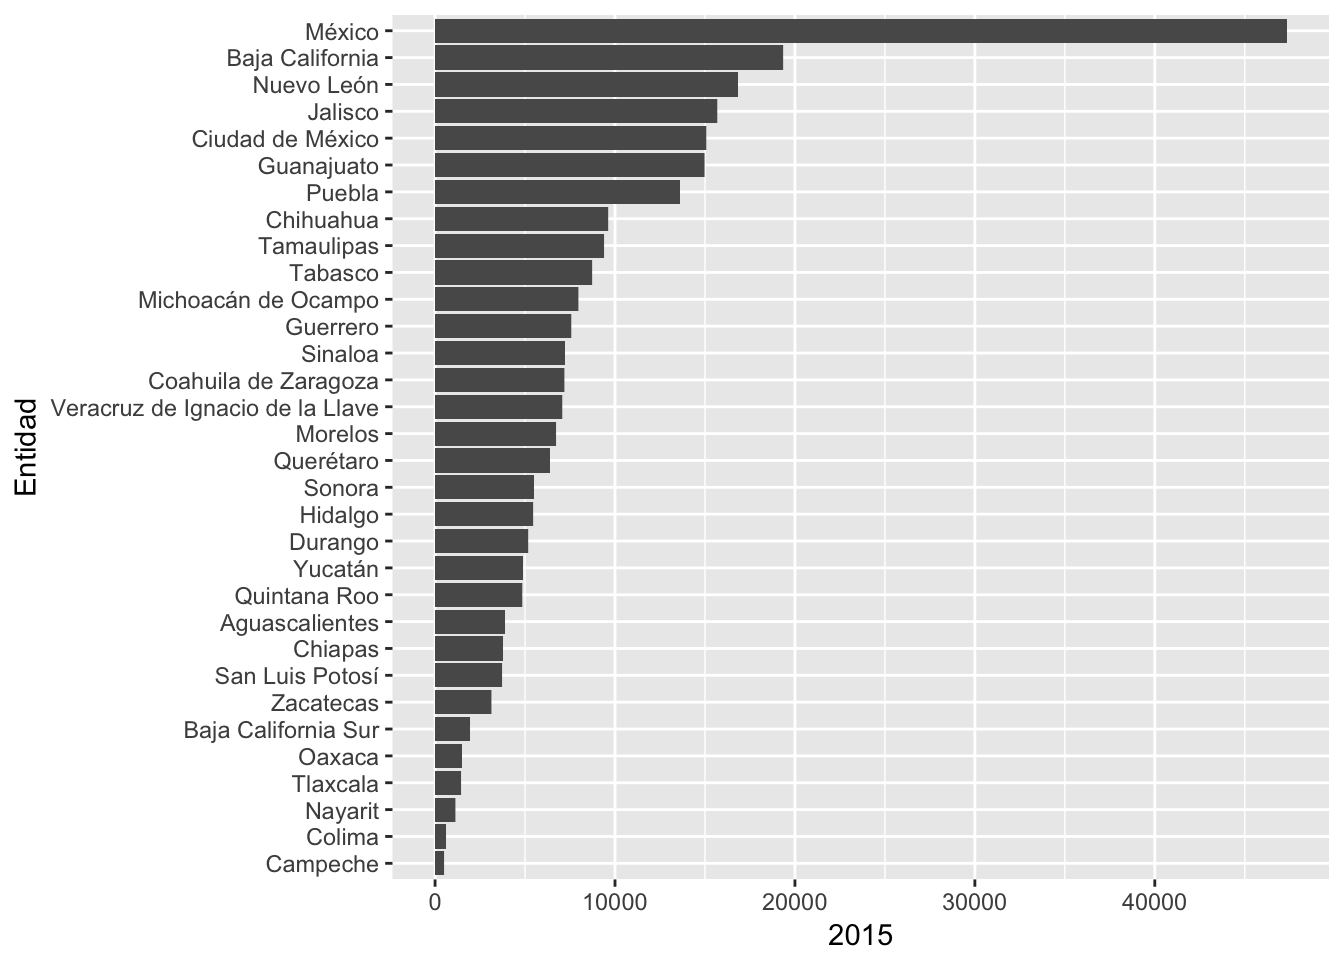
\includegraphics{bookdown-demo_files/figure-latex/unnamed-chunk-89-1.pdf}
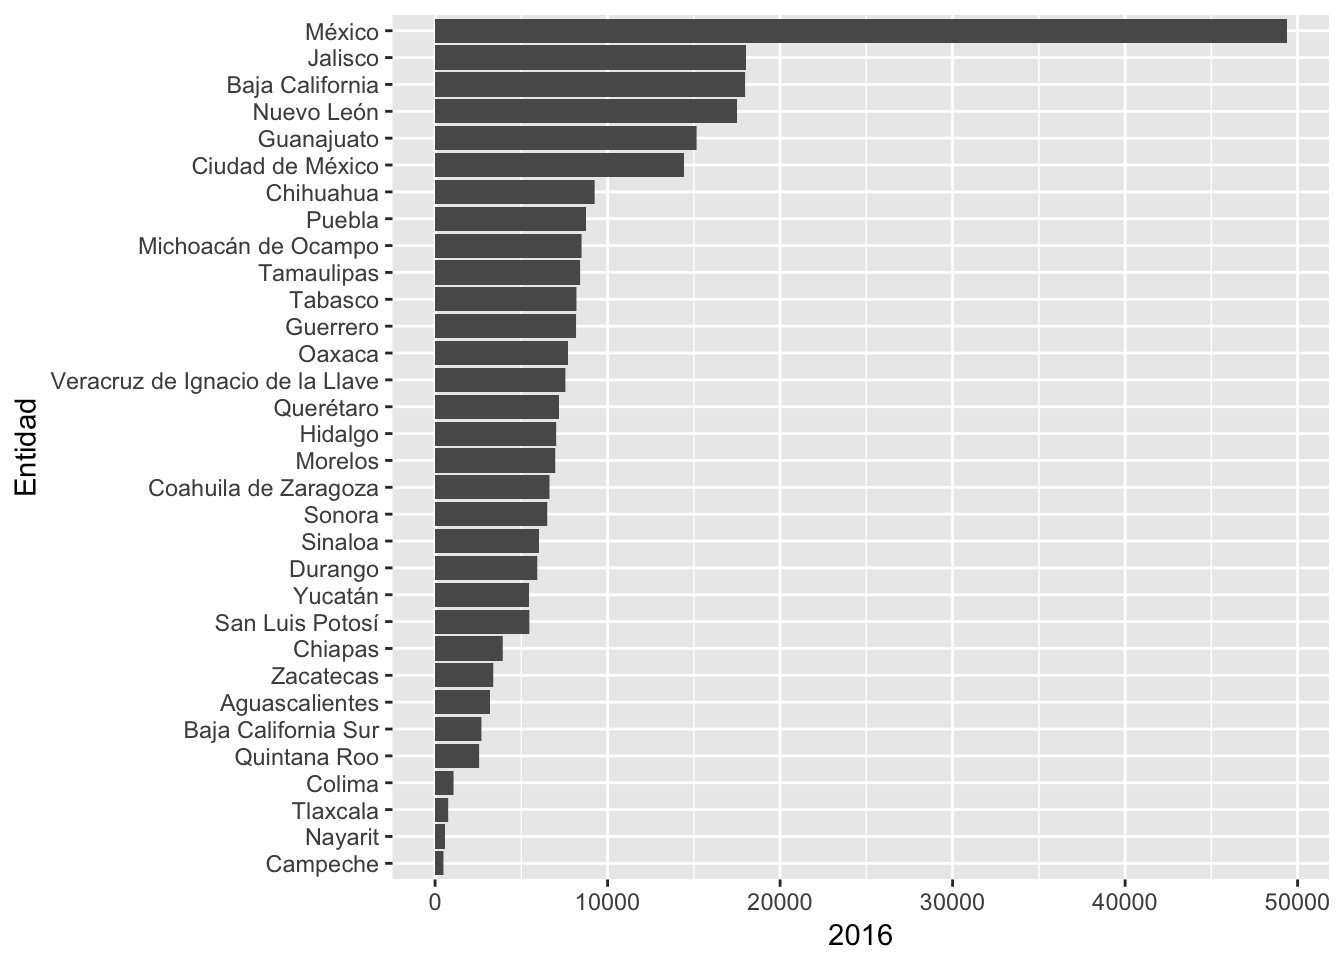
\includegraphics{bookdown-demo_files/figure-latex/unnamed-chunk-89-2.pdf}
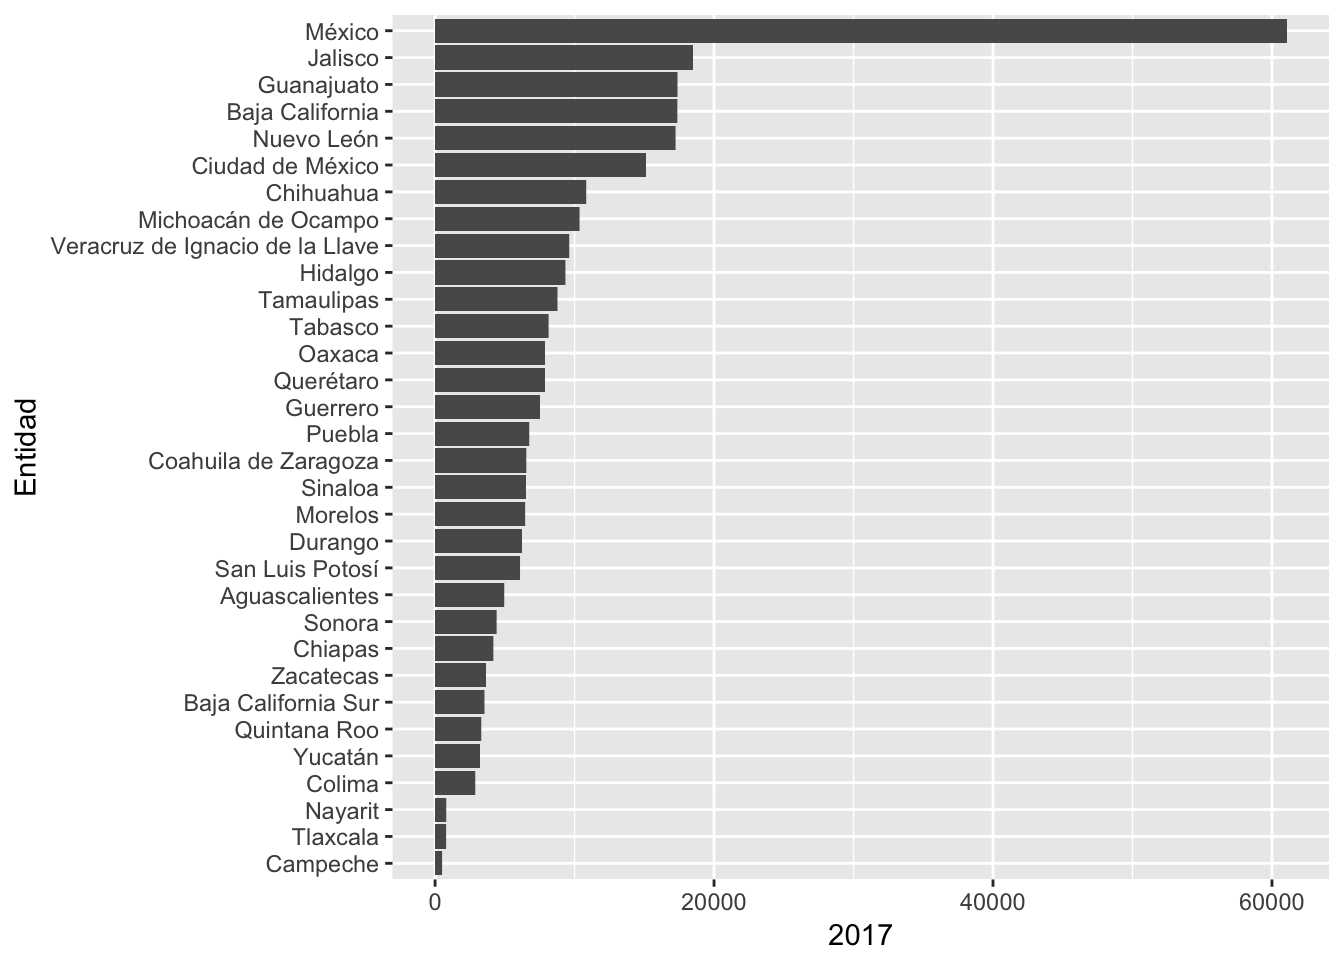
\includegraphics{bookdown-demo_files/figure-latex/unnamed-chunk-89-3.pdf}
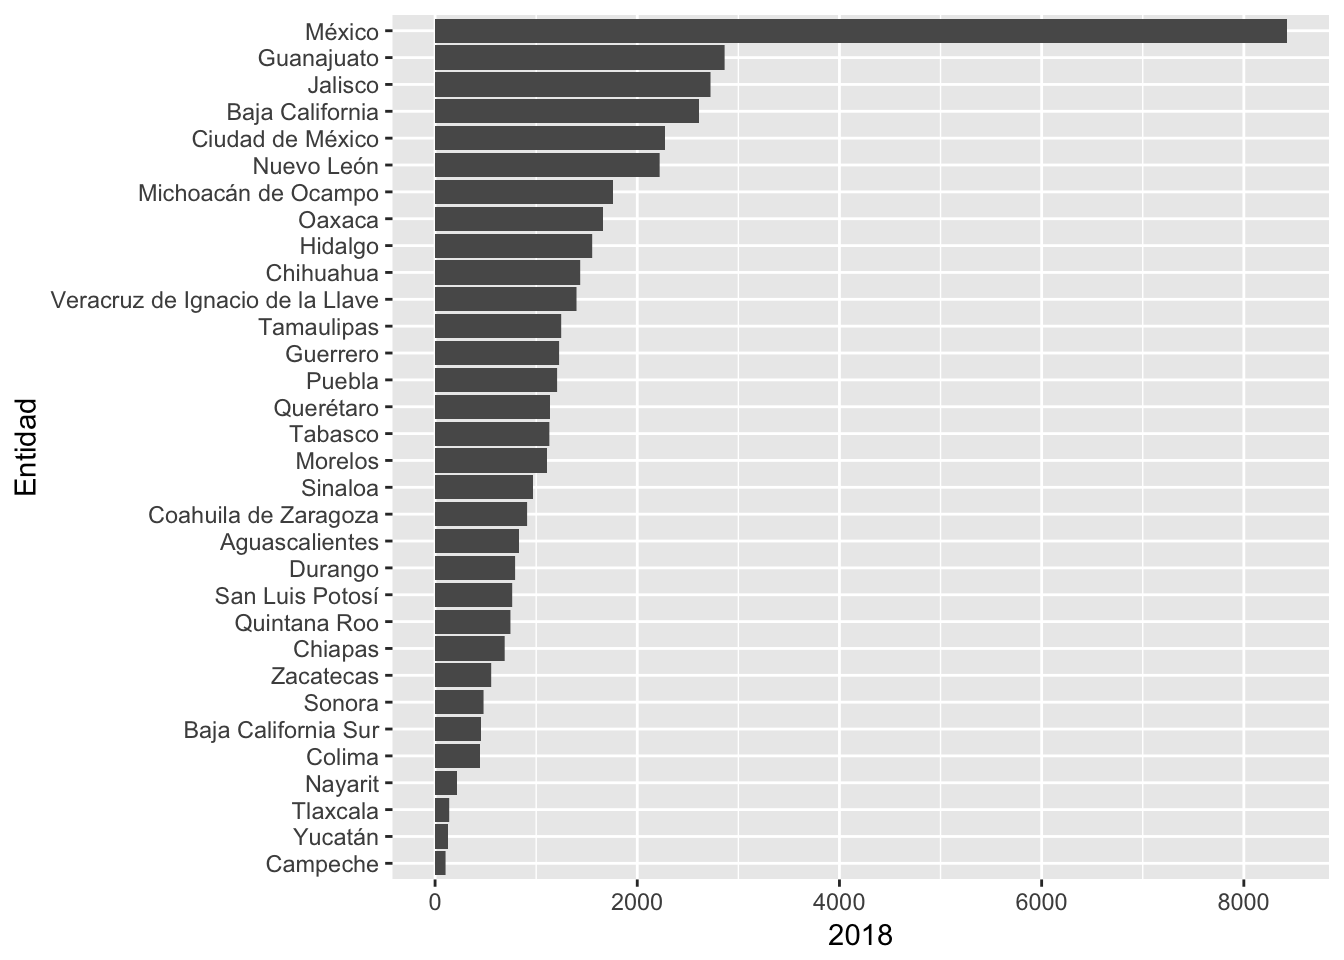
\includegraphics{bookdown-demo_files/figure-latex/unnamed-chunk-89-4.pdf}

\subsubsection{\texorpdfstring{Bucle
\emph{while}}{Bucle while}}\label{bucle-while}

While es otro tipo de bucle que se usa cuando no se conoce de antemano
el número de itearaciones que se harán. ¿En qué contexto puede ocurrir
esto? Usualmente ocurre en problemas de simulación o muestreo, por
ejemplo:

Si quisieramos simular un dado:

\begin{Shaded}
\begin{Highlighting}[]
\NormalTok{dado <-}\StringTok{ }\ControlFlowTok{function}\NormalTok{(x) \{}
  \KeywordTok{sample}\NormalTok{(}\DecValTok{1}\OperatorTok{:}\DecValTok{6}\NormalTok{, }\DecValTok{1}\NormalTok{, }\DataTypeTok{replace=}\OtherTok{TRUE}\NormalTok{)}
\NormalTok{\}}
\end{Highlighting}
\end{Shaded}

Ahora pensamos que nos interesa una muestra de tamaño 10 de tiros de dos
dados, pero con la particularidad de que la suma de los números sea
menor que 8:

\begin{Shaded}
\begin{Highlighting}[]
\NormalTok{lanzamientos <-}\StringTok{ }\KeywordTok{list}\NormalTok{()}

\ControlFlowTok{while}\NormalTok{(}\KeywordTok{length}\NormalTok{(lanzamientos) }\OperatorTok{<}\StringTok{ }\DecValTok{10}\NormalTok{) \{}
\NormalTok{  dado_a <-}\StringTok{ }\KeywordTok{dado}\NormalTok{()}
\NormalTok{  dado_b <-}\StringTok{ }\KeywordTok{dado}\NormalTok{()}
  \ControlFlowTok{if}\NormalTok{(dado_a }\OperatorTok{+}\StringTok{ }\NormalTok{dado_b }\OperatorTok{<}\StringTok{ }\DecValTok{8}\NormalTok{) \{}
\NormalTok{    lanzamientos <-}\StringTok{ }\KeywordTok{c}\NormalTok{(lanzamientos, }\KeywordTok{list}\NormalTok{(}\KeywordTok{c}\NormalTok{(dado_a, dado_b)))}
\NormalTok{  \}}
\NormalTok{\}}


\NormalTok{lanzamientos}
\end{Highlighting}
\end{Shaded}

\begin{verbatim}
## [[1]]
## [1] 3 3
## 
## [[2]]
## [1] 5 1
## 
## [[3]]
## [1] 4 1
## 
## [[4]]
## [1] 1 2
## 
## [[5]]
## [1] 1 3
## 
## [[6]]
## [1] 5 1
## 
## [[7]]
## [1] 3 3
## 
## [[8]]
## [1] 1 1
## 
## [[9]]
## [1] 1 2
## 
## [[10]]
## [1] 1 1
\end{verbatim}

\subsection{Iteración funcional}\label{iteracion-funcional}

Ya se introdujo la idea de que se puede utilizar una función dentro de
otra función. En esta sección se aprenderá a utilizar el paquete purr,
que elimina la necesidad de aprender a generar bucles complejos. La base
de R tiene funciones con la misma idea (apply(), lapply(), tapply(),
etc) pero purr tiende a ser más consistente y por lo tanto más fácil de
aprender a usar.

Si se quiere indagar en las funcones apply se puede consultar esta liga:

\url{https://www.datacamp.com/community/tutorials/r-tutorial-apply-family\#gs.bJ=BAKY}

El objetivo de las funciones de purr es ayudar a romper las tareas de
manipulación de listas en pedazos independientes:

Primero se debe plantear la interrogante ¿Cómo se puede resolver el
problema de interés para un único elemento de la lista? Luego purr ayuda
a generalizarlo a cada elemento de la lista.

\paragraph{La función map}\label{la-funcion-map}

La tarea de barrer un vector, hacer algo a cada elemento y luego guardar
los resultados es tan común que el paquete purr provee una familia de
funciones para llevar esto a cabo.

Existe una función para cada tipo de salida:

\begin{itemize}
\tightlist
\item
  map() genera una lista.
\item
  map\_lgl() genera un vector de valores lógicos.
\item
  map\_int() genera un vector de valores enteros.
\item
  map\_dbl() genera un vector de valores dobles (números reales).
\item
  map\_chr() genera un vector de valores texto.
\end{itemize}

Cada una de estas funciones recibe como entrada un vector, aplica una
función elegida por el usuario a cada pedazo y regresa un vector de la
misma longitud que el original (y con los mismos nombres).

Por ejemplo para calcular la media de cada columna de la tabla de datos
de coches basta con hacer

\begin{Shaded}
\begin{Highlighting}[]
\KeywordTok{map_dbl}\NormalTok{(mtcars, mean)}
\end{Highlighting}
\end{Shaded}

Supongamos que tenemos ahora diversas fuentes de datos que queremos
operear en paralelo.

\begin{Shaded}
\begin{Highlighting}[]
\NormalTok{x <-}\StringTok{ }\KeywordTok{c}\NormalTok{(}\DecValTok{1}\NormalTok{, }\DecValTok{2}\NormalTok{, }\DecValTok{3}\NormalTok{, }\DecValTok{4}\NormalTok{, }\DecValTok{5}\NormalTok{, }\DecValTok{6}\NormalTok{, }\DecValTok{7}\NormalTok{, }\DecValTok{8}\NormalTok{, }\DecValTok{9}\NormalTok{, }\DecValTok{10}\NormalTok{)}
\NormalTok{y <-}\StringTok{ }\KeywordTok{c}\NormalTok{(}\DecValTok{32}\NormalTok{, }\DecValTok{54}\NormalTok{, }\DecValTok{52}\NormalTok{, }\DecValTok{53}\NormalTok{, }\DecValTok{67}\NormalTok{, }\DecValTok{89}\NormalTok{, }\DecValTok{100}\NormalTok{, }\DecValTok{54}\NormalTok{, }\DecValTok{75}\NormalTok{, }\DecValTok{27}\NormalTok{)}


\NormalTok{z <-}\StringTok{ }\KeywordTok{map2_dbl}\NormalTok{(x, y, }\ControlFlowTok{function}\NormalTok{(x,y)\{ }\KeywordTok{return}\NormalTok{(x }\OperatorTok{+}\StringTok{ }\NormalTok{y) \})}
\NormalTok{z}
\end{Highlighting}
\end{Shaded}

Para evitar la declaración de la función que suma dentro de la llamada
podemos hacer:

\begin{Shaded}
\begin{Highlighting}[]
\NormalTok{mi_suma <-}\StringTok{ }\ControlFlowTok{function}\NormalTok{(x,y)\{ }
  \KeywordTok{return}\NormalTok{(x }\OperatorTok{+}\StringTok{ }\NormalTok{y) }
\NormalTok{\}}

\NormalTok{z <-}\StringTok{ }\KeywordTok{map2_dbl}\NormalTok{(x, y, mi_suma)}
\NormalTok{z}
\end{Highlighting}
\end{Shaded}

Pero el paquete purrr (parte del tidyverse) permite una sintaxis
especial. Sustituimos la palabra \emph{function} por una
``\textasciitilde{}'' y accesamos a las variables de entrada por medio
del placeholder ``.'':

\begin{Shaded}
\begin{Highlighting}[]
\NormalTok{z <-}\StringTok{ }\KeywordTok{map2_dbl}\NormalTok{(x, y, }\OperatorTok{~}\StringTok{ }\NormalTok{.x }\OperatorTok{+}\StringTok{ }\NormalTok{.y)}
\NormalTok{z}
\end{Highlighting}
\end{Shaded}


\includegraphics{./imagenes/manicule2.jpg} Ejercicio: ¿Qué diferencia
hay entre usar la función map2\_dbl y la función map2?


\includegraphics{./imagenes/manicule2.jpg} Ejercicio: Existe un análogo
a la función map2 para más fuentes de datos llamada pmap. Escribe un
ejemplo para sumar 3 vectores usando esta función.

\paragraph{La función walk}\label{la-funcion-walk}

Es una alternativa a map cuando se quiere llamar una función más por sus
efectos que por sus resultados. Esto es, sirve para llevar a cabo un
proceso a lo largo de, por ejemplo, un vector.

Un ejemplo muy simple

\begin{Shaded}
\begin{Highlighting}[]
\NormalTok{x <-}\StringTok{ }\KeywordTok{list}\NormalTok{(}\DecValTok{7}\NormalTok{, }\StringTok{"a"}\NormalTok{, }\DecValTok{6}\NormalTok{, }\StringTok{"gatito"}\NormalTok{)}

\NormalTok{x }\OperatorTok\StringTok{ }
\StringTok{  }\KeywordTok{walk}\NormalTok{(print)  }\CommentTok{# si se fijan hace algo muy parecido a nuestro primer ejemplo de bucle}
\end{Highlighting}
\end{Shaded}

Las funciones map() y walk() iteran sobre múltiples arugmentos en
paralelo, map2() y walk2() se especializan en el caso particular de 2
argumentos y pmap() y pwalk() en el caso de un número ilimitado de
argumentos en una lista. La función walk, en general, no es tan útil
como las funciones walk2() or pwalk().

Para replicar el ejercicio de separar la tabla de datos de homicidios se
puede usar map() seguido de pwalk() para además guardar los plots como
pdf.

\begin{Shaded}
\begin{Highlighting}[]
\NormalTok{plots <-}\StringTok{ }\NormalTok{datos }\OperatorTok\StringTok{ }
\StringTok{         }\KeywordTok{split}\NormalTok{(.}\OperatorTok{$}\NormalTok{Año) }\OperatorTok\StringTok{ }\CommentTok{# nota importante: "." al usar map sirve para algo análogo a "i" en los bucles}
\StringTok{         }\KeywordTok{map}\NormalTok{(}\OperatorTok{~}\KeywordTok{ggplot}\NormalTok{(}\DataTypeTok{data =}\NormalTok{ ., }\KeywordTok{aes}\NormalTok{(}\DataTypeTok{x =} \KeywordTok{reorder}\NormalTok{(Entidad, Total), }\DataTypeTok{y =}\NormalTok{ Total)) }\OperatorTok{+}\StringTok{ }
\StringTok{                                       }\KeywordTok{geom_bar}\NormalTok{(}\DataTypeTok{stat =} \StringTok{"identity"}\NormalTok{) }\OperatorTok{+}\StringTok{ }
\StringTok{                                       }\KeywordTok{labs}\NormalTok{(}\DataTypeTok{y=}\NormalTok{.}\OperatorTok{$}\NormalTok{Año, }\DataTypeTok{x=}\StringTok{"Entidad"}\NormalTok{) }\OperatorTok{+}\StringTok{ }
\StringTok{                                       }\KeywordTok{coord_flip}\NormalTok{())}


\KeywordTok{print}\NormalTok{(plots)}
\end{Highlighting}
\end{Shaded}

\begin{verbatim}
## $`2015`
\end{verbatim}

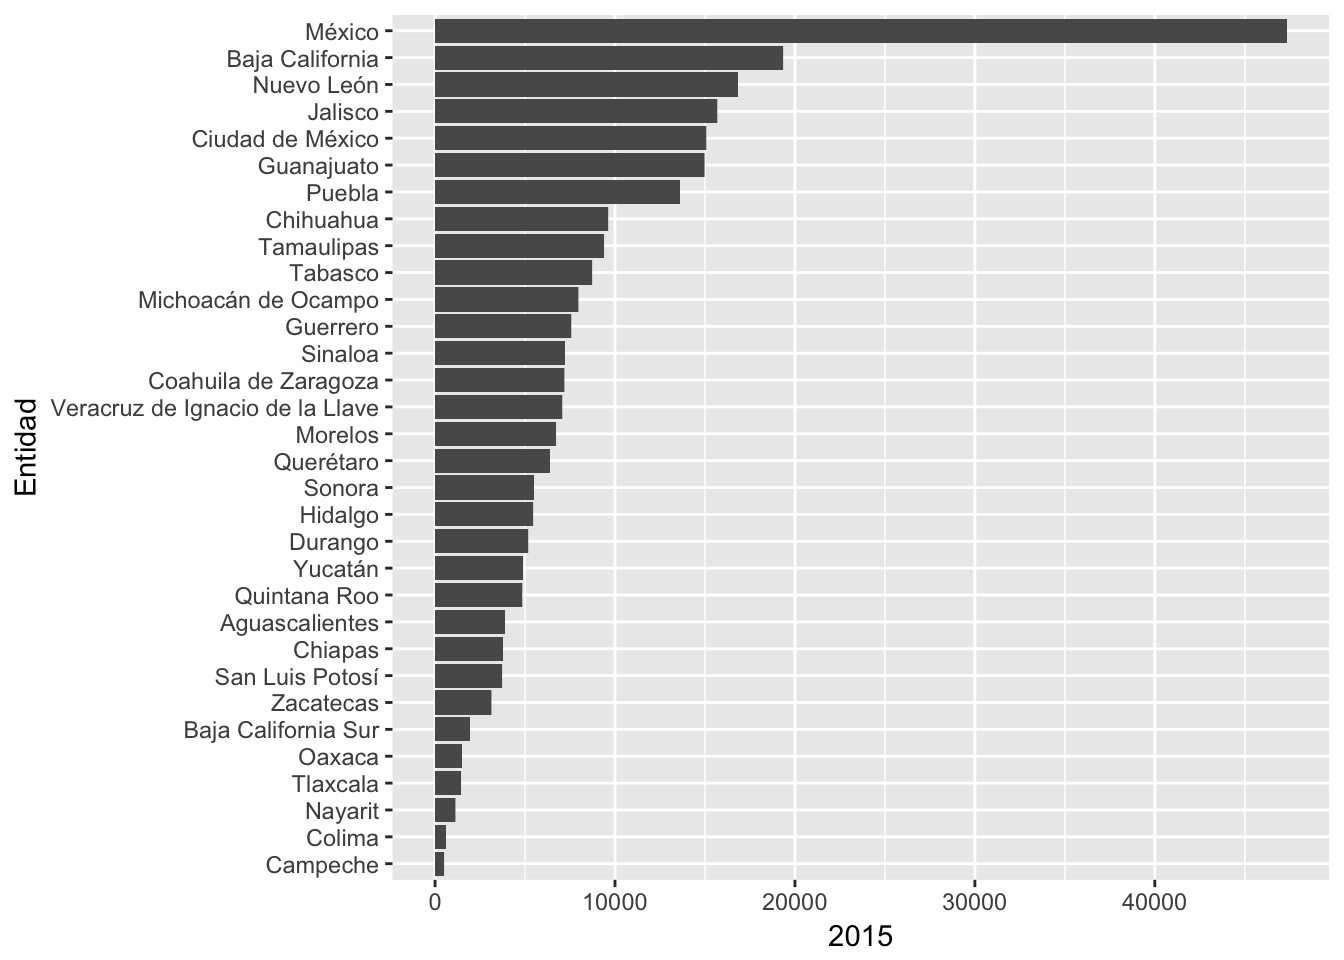
\includegraphics{bookdown-demo_files/figure-latex/unnamed-chunk-97-1.pdf}

\begin{verbatim}
## 
## $`2016`
\end{verbatim}

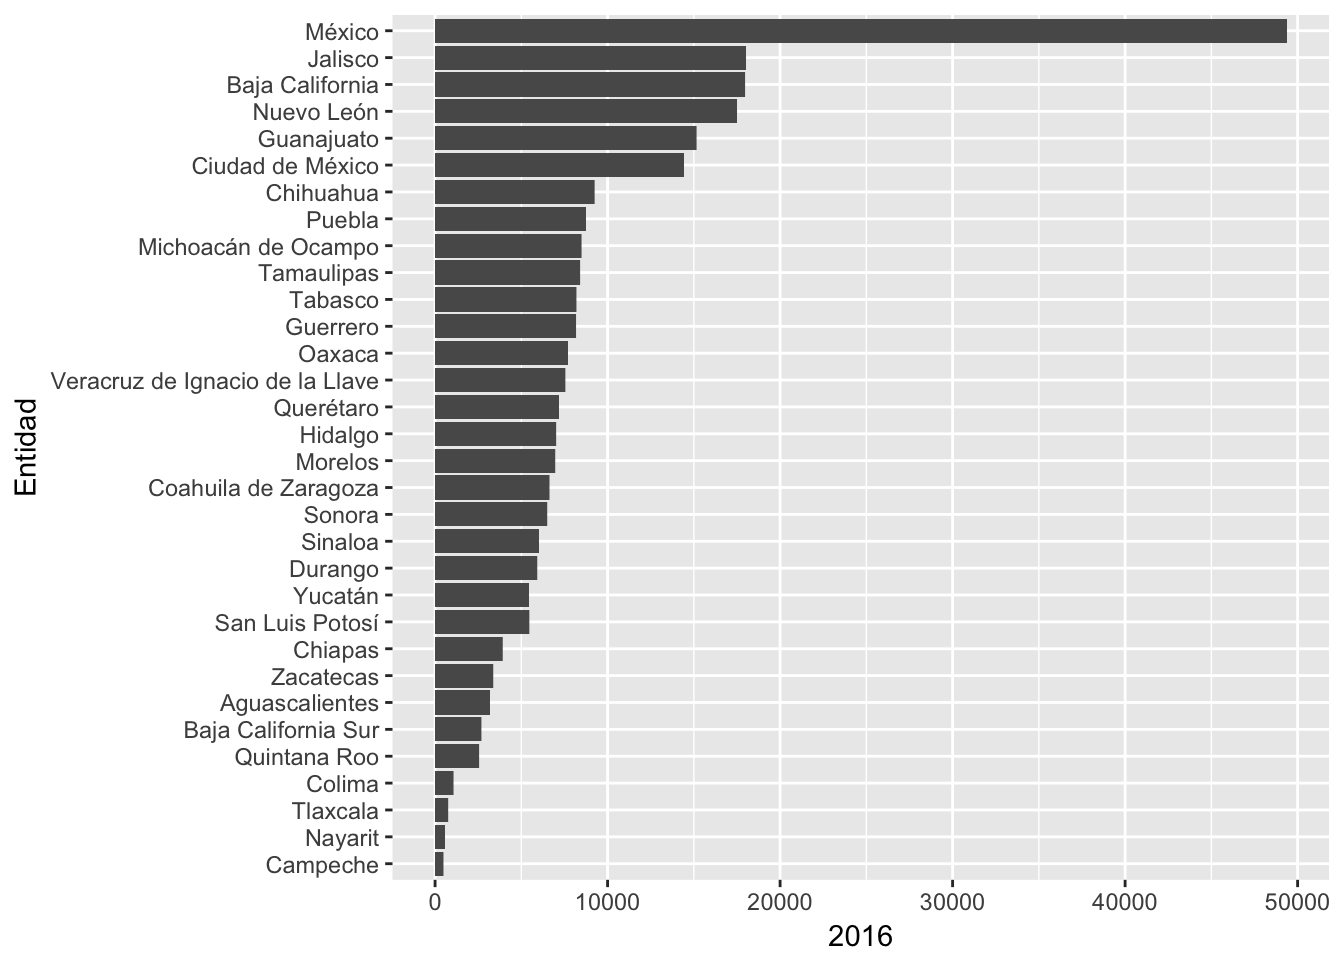
\includegraphics{bookdown-demo_files/figure-latex/unnamed-chunk-97-2.pdf}

\begin{verbatim}
## 
## $`2017`
\end{verbatim}

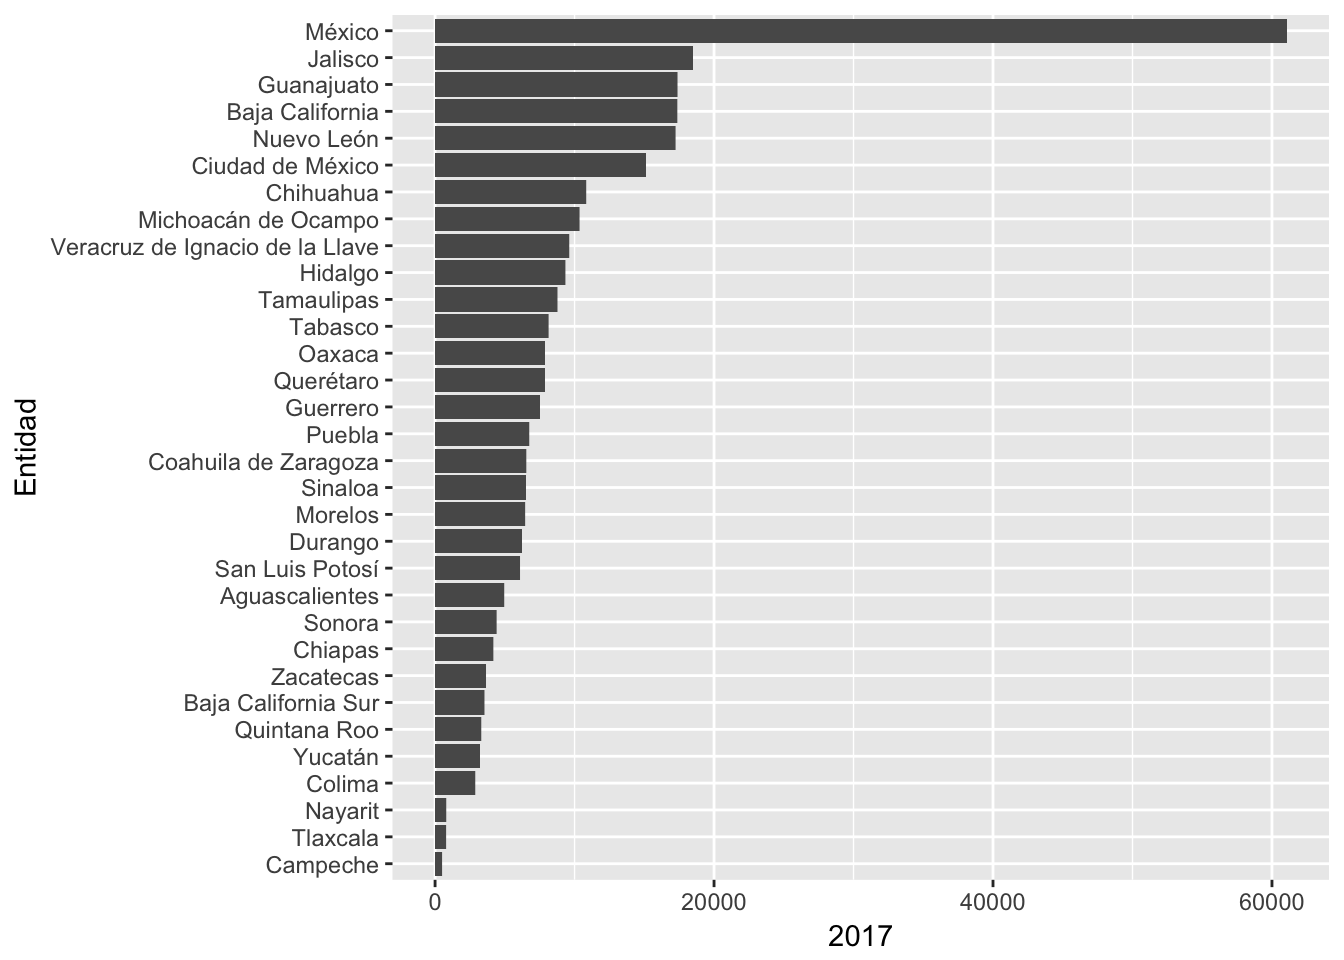
\includegraphics{bookdown-demo_files/figure-latex/unnamed-chunk-97-3.pdf}

\begin{verbatim}
## 
## $`2018`
\end{verbatim}

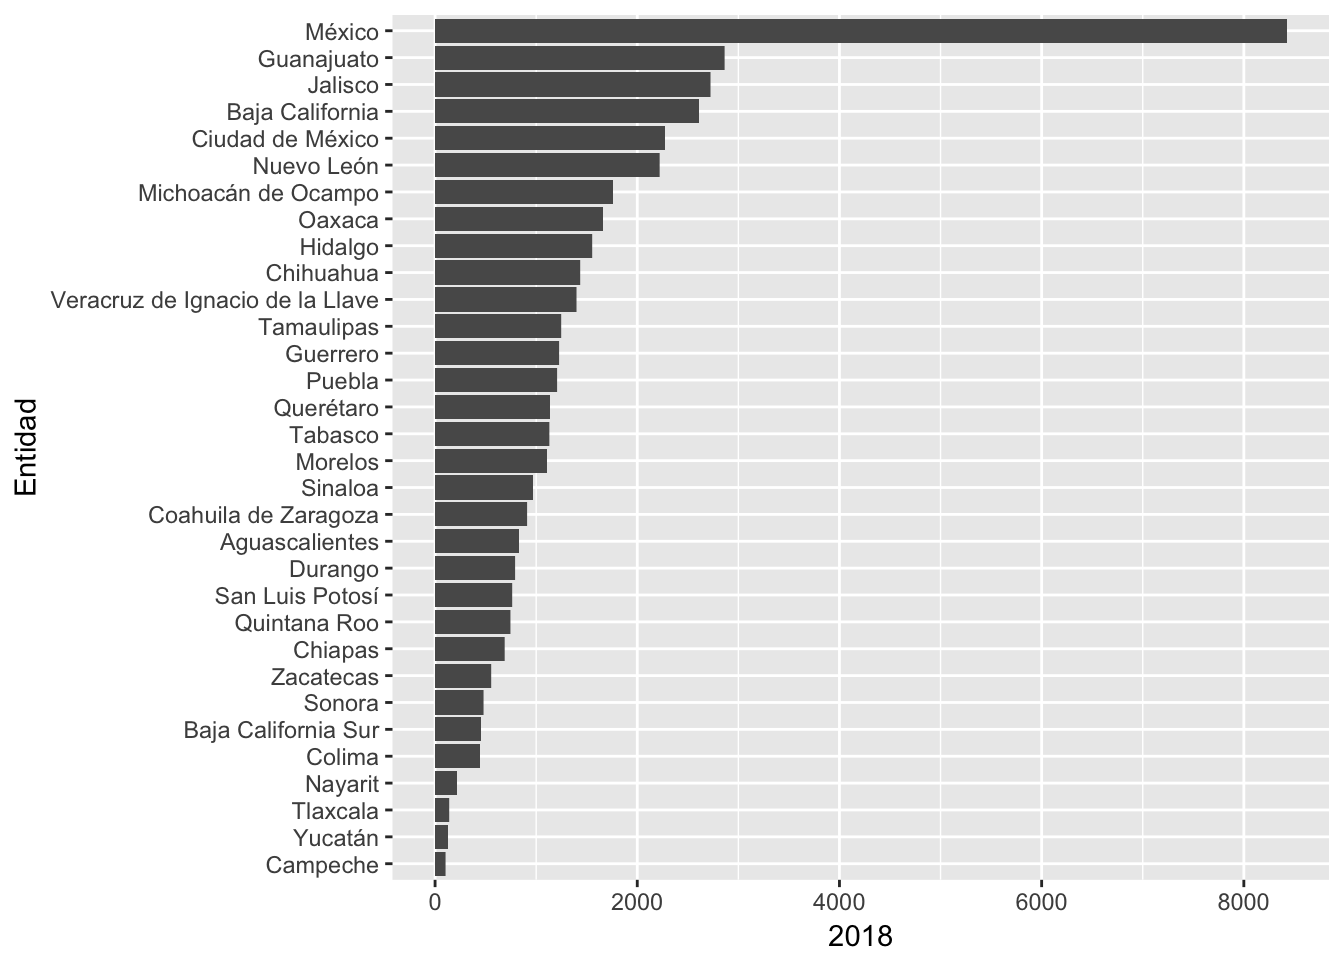
\includegraphics{bookdown-demo_files/figure-latex/unnamed-chunk-97-4.pdf}

\begin{Shaded}
\begin{Highlighting}[]
\NormalTok{paths <-}\StringTok{ }\NormalTok{stringr}\OperatorTok{::}\KeywordTok{str_c}\NormalTok{(}\KeywordTok{names}\NormalTok{(plots), }\StringTok{".pdf"}\NormalTok{)}
\KeywordTok{pwalk}\NormalTok{(}\KeywordTok{list}\NormalTok{(paths, plots), ggsave, }\DataTypeTok{path =} \KeywordTok{getwd}\NormalTok{())}
\KeywordTok{getwd}\NormalTok{()}
\end{Highlighting}
\end{Shaded}


\includegraphics{./imagenes/manicule2.jpg} Tarea: desarrollar un script
que incluya una función que lleve a cabo un proceso que generalmente
llevarías a cabo usando otra herramienta, por ejemplo excel, sobre una
tabla de datos propia. Explicar lo que se llevó a cabo.

\chapter{Modelado}\label{modelado}

\section{¿Qué aprendimos la clase
pasada?}\label{que-aprendimos-la-clase-pasada-4}

\begin{itemize}
\tightlist
\item
  Cómo analizar muestras complejas en R
\end{itemize}

En esta clase aprenderemos a:

\begin{itemize}
\tightlist
\item
  Utilizar modelos estadísticos para exploración de datos y para probar
  hipótesis.
\end{itemize}

\section{Modelos}\label{modelos}

El objetivo primordial de los modelos estadísticos es el de proveer un
sumario simple de baja dimensión de un conjunto de datos.

Idealmente un modelo captura la señal de interés (los patrones reals y
generales del fenómeno que queremos estudiar) e ignora el ``ruido''
(e.g.~variación aleatoria que no es de nuestro interés).

Vamos a proceder a estudiar cuál es la mecánica detrás de los modelos
estadísticos concentrándonos en una familia muy importante de ellos: los
modelos lineales.

\subsection{Generación de hipótesis vs confirmación de
hipótesis}\label{generacion-de-hipotesis-vs-confirmacion-de-hipotesis}

Tradicionalmente, el objetivo del modelado estadístico fue la
inferencia:plantear y comprobar hipótesis. Hacer esto correctamente no
es complicado pero es difícil.

Hay que entender un par de ideas para poder llevar a cabo inferencia de
una manera correcta:

\begin{itemize}
\item
  Cada observación de nuestro conjunto de datos base se puede usar para
  exploración o para confirmación pero nunca para ambas.
\item
  Puedes usar una observación las veces que quieras para exploración,
  pero sólo la puedes usar una vez para confirmación. En cuanto uses una
  observación más de una vez estás automáticamente participando en un
  ejercicio exploratorio y no de confirmación.
\end{itemize}

Esto es necesario porque para confirmar una hipótesis se deben de usar
datos independientes a los que se usaron para generar la hipótesis. De
otra manera se está siendo optimista en cuanto a la solidéz de la
hipótesis.

Se verá más adelante pero para llevar a cabo un análisis de confirmación
para modelos estadísticos una manera de proceder es partiendo tu
conjunto de datos en tres subconjuntos:

\begin{itemize}
\item
  \textasciitilde{}60\% para explorar y entrenar tu modelo. Tienes
  permitido hacer lo que sea con este subconjunto de tus datos:
  manipularlo a gusto, visualizarlo, ajustarle un montón de modelos,
  etc.
\item
  \textasciitilde{}20\% un conjunto de consulta. Sirve para comparar
  modelos o visualizaciones, pero no está permitido usarlo en el ajuste
  de modelos.
\item
  \textasciitilde{}20\% es el conjunto de prueba final. Sólo se puede
  usar este conjunto de datos UNA vez, para probar tu modelo final.
\end{itemize}

Esta partición permite explorar tus datos de entrenamiento,
ocasionalmente generando hipótesis candidatas que se contrastan usando
el conjunto de consulta. Cuando se tiene confianza en tener un buen
modelo, se puede evaluar en el conjunto de prueba.

\subsection{Especificación de modelos}\label{especificacion-de-modelos}

Hay dos partes fundamentales en un modelo:

\begin{itemize}
\tightlist
\item
  Primero, se define una familia de modelos que expresa de manera
  precisa, pero genérica, el patrón que se quiere capturar. Por ejemplo
  el patrón puede ser una línea recta:
\end{itemize}

\[ Y = \beta_{0} + \beta_{1}*X \]

Aquí, Y y X son variables conocidos de tus datos. \(\beta_{0}\) y
\(\beta_{1}\) son parámetros que pueden capturar distintos patrones.

\begin{itemize}
\tightlist
\item
  Luego, en el ejercicio de modelado se encuentran los parámetros a la
  hora de ajustar el modelo, de manera tal que el modelo se encuentre
  ``lo más cerca posible'' a tus datos, por ejemplo:
\end{itemize}

\[ Y = 3 + 11X \]

Es importante recalcar que el modelo ajustado es el modelo más cercano a
tus datos pero de una familia particular de modelos escogida a priori.
Esto implica que se tiene el ``mejor'' modelo dado un cierto criterio
muy particular. Definitivamente no implica que se tiene un buen modelo o
que el modelo es ``cierto'':

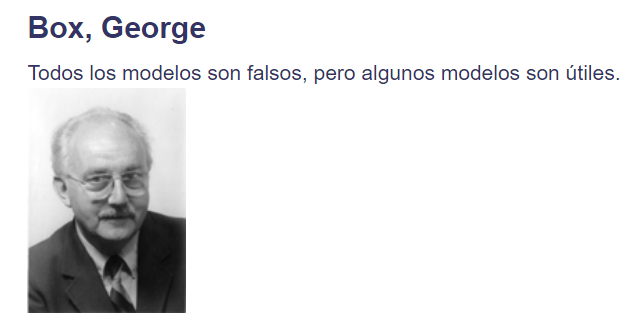
\includegraphics[width=8.85in]{./imagenes/box}

\subsection{Un primer modelo simple}\label{un-primer-modelo-simple}

Echémosle un vistazo a el conjunto de datos simulados sim1 (vienen en el
tidyverse)

\begin{Shaded}
\begin{Highlighting}[]
\CommentTok{# carguemos los paquetes}

\KeywordTok{library}\NormalTok{(tidyverse)}

\KeywordTok{library}\NormalTok{(modelr)}

\KeywordTok{head}\NormalTok{(sim1)}
\end{Highlighting}
\end{Shaded}

\begin{verbatim}
## # A tibble: 6 x 2
##       x     y
##   <int> <dbl>
## 1     1  4.20
## 2     1  7.51
## 3     1  2.13
## 4     2  8.99
## 5     2 10.2 
## 6     2 11.3
\end{verbatim}

Como podrán ver, consta de dos variables continuas únicamente (x,y).

Podemos usar lo aprendido en clases pasadas para visualizar la relación
entre estas dos variables:

\begin{Shaded}
\begin{Highlighting}[]
\KeywordTok{ggplot}\NormalTok{(sim1, }\KeywordTok{aes}\NormalTok{(x, y)) }\OperatorTok{+}\StringTok{ }
\StringTok{  }\KeywordTok{geom_point}\NormalTok{()}
\end{Highlighting}
\end{Shaded}

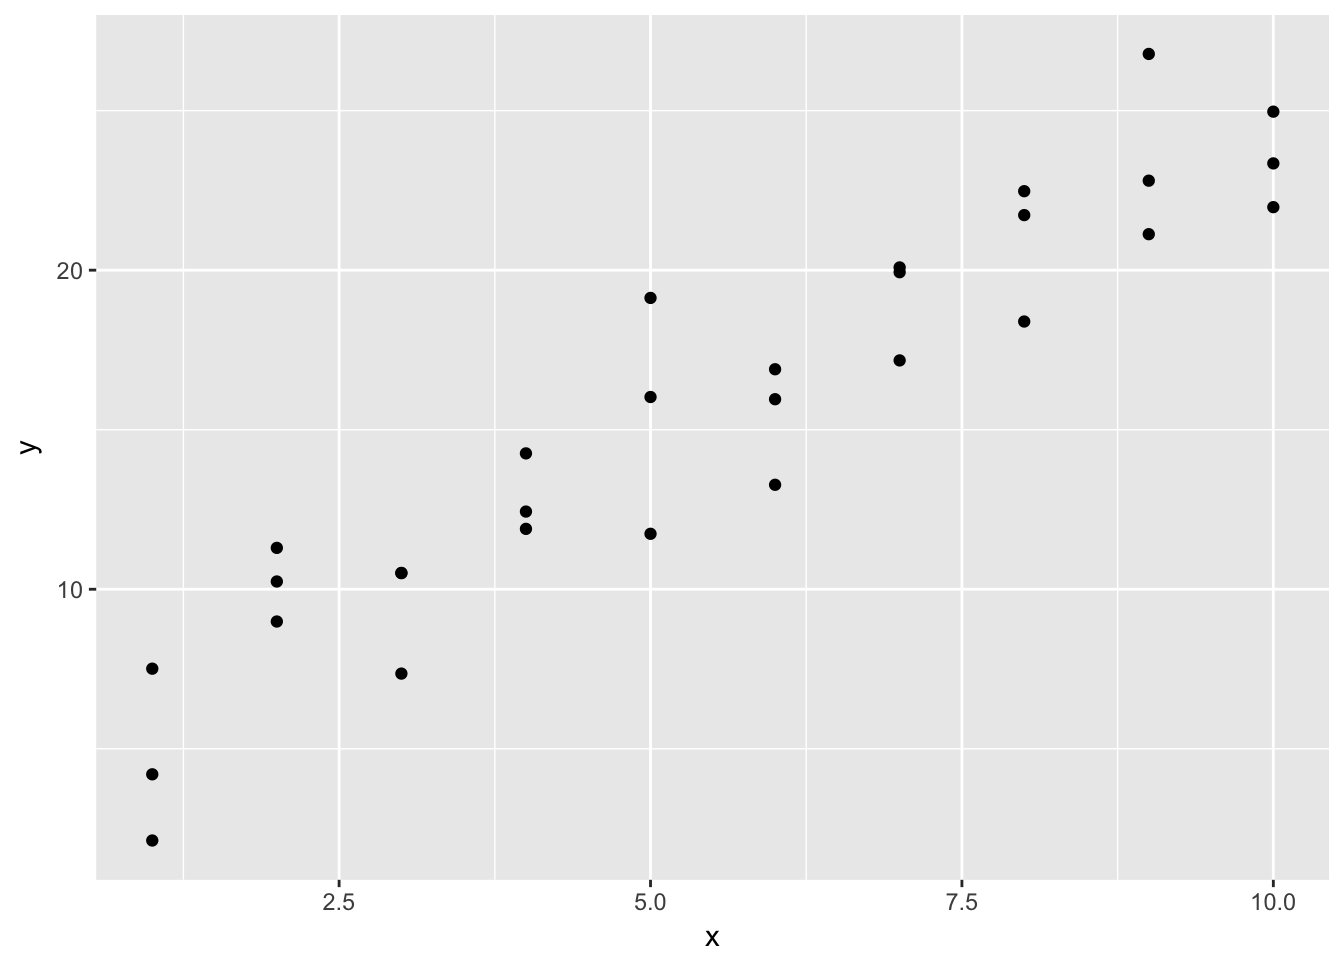
\includegraphics{bookdown-demo_files/figure-latex/unnamed-chunk-101-1.pdf}

Es claro que existe un patrón fuerte entre las dos variables (¿Qué
tipo?).

Ahora es nuestra tarea proponer un modelo para este conjunto de datos
que capture el patrón de la mejor manera posible.


\includegraphics{./imagenes/manicule2.jpg} Usar la función runif(),
consultar su ayuda y explicar con sus palabras qué hace.

La función anterior nos dejará generar una gran cantidad de parámetros
para producir modelos candidatos (como hemos venido trabajando sólo son
dos parámetros los que requerimos para datos con dos variables).

\begin{Shaded}
\begin{Highlighting}[]
\CommentTok{# parametros}
\NormalTok{modelos <-}\StringTok{ }\KeywordTok{tibble}\NormalTok{(}
  \DataTypeTok{beta0 =} \KeywordTok{runif}\NormalTok{(}\DecValTok{250}\NormalTok{, }\OperatorTok{-}\DecValTok{20}\NormalTok{, }\DecValTok{40}\NormalTok{),}
  \DataTypeTok{beta1 =} \KeywordTok{runif}\NormalTok{(}\DecValTok{250}\NormalTok{, }\OperatorTok{-}\DecValTok{5}\NormalTok{, }\DecValTok{5}\NormalTok{)}
\NormalTok{)}

\KeywordTok{ggplot}\NormalTok{(sim1, }\KeywordTok{aes}\NormalTok{(x, y)) }\OperatorTok{+}\StringTok{ }
\StringTok{  }\KeywordTok{geom_abline}\NormalTok{(}\KeywordTok{aes}\NormalTok{(}\DataTypeTok{intercept =}\NormalTok{ beta0, }\DataTypeTok{slope =}\NormalTok{ beta1), }\DataTypeTok{data =}\NormalTok{ modelos, }\DataTypeTok{alpha =} \DecValTok{1}\OperatorTok{/}\DecValTok{4}\NormalTok{) }\OperatorTok{+}
\StringTok{  }\KeywordTok{geom_point}\NormalTok{()}
\end{Highlighting}
\end{Shaded}

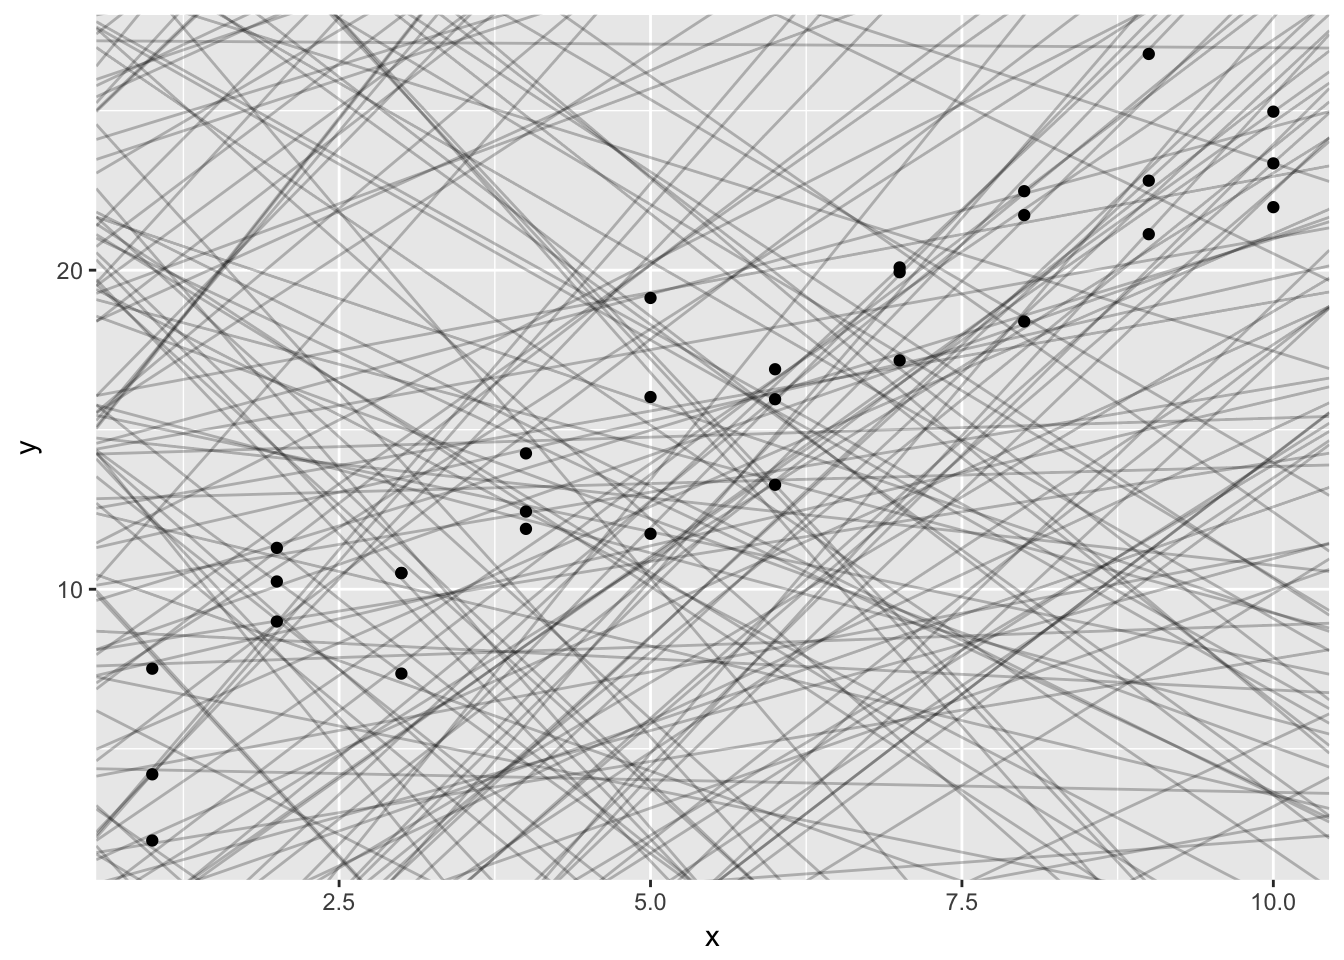
\includegraphics{bookdown-demo_files/figure-latex/unnamed-chunk-102-1.pdf}

Pintamos 250 modelos candidatos sobre nuestros datos simulados ¡Muchos
de ellos son realmente malos!

¿Cómo le hacemos para encontrar un buen modelo? ¿Cómo se formaliza la
idea de que un buen modelo es uno que está ``cerca'' de nuestros datos?
Necesitamos una manera de cuantificar la distancia de un modelo
candidato a nuestros datos.Luego podemos buscar un modelo que encuentre
valors para \(\beta_{0}\) y \(\beta_{1}\) de manera tal que el modelo
esté a la menor distancia posible de los datos.

Un buen lugar para empezar es encontrar la distancia vertical de cada
punto de nuestros datos a nuestro modelo (en este caso una línea recta).

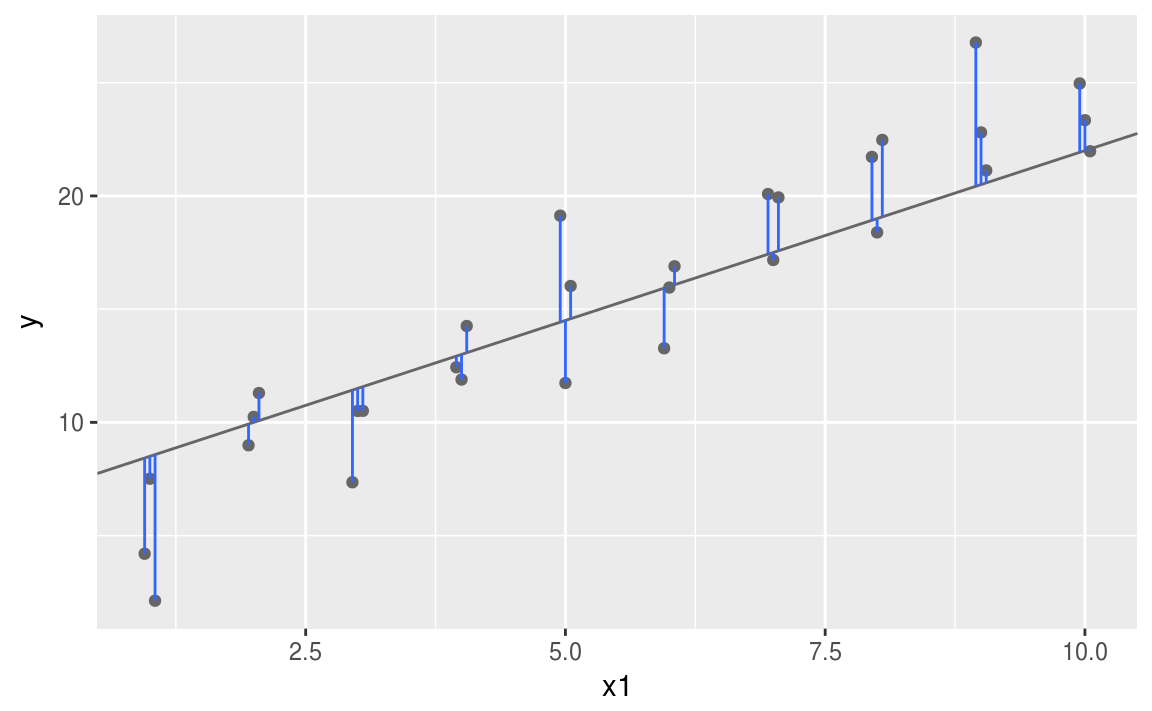
\includegraphics[width=16in]{./imagenes/dists}

La intuición detrás de el ajuste de varias familias de modelos es que si
puedes establecer una función que defina la distancia entre el modelo y
el conjunto de datos, entonces un algoritmo puede minimzar tal
distancia, efectivamente encontrando los mejores parámetros para tu
modelo. Una muy común es la suma de los cuadrados de las distancias
verticales antes mostradas, eso se denomina ajuste por mínimos
cuadrados.

R tiene varias herramientas y paquetes para trabajar con modelos. Una
función clásica es lm() que permite ajustar modelos lineales como los
que hemos venido viendo. R tiene varias manera de especificar los
modelos que se buscan ajustar. Por ejemplo, con una estructura llamada
fórmula: Y \textasciitilde{} X que se traduce en:

\[ Y = \beta_{0} + \beta_{1}*X \]

\begin{Shaded}
\begin{Highlighting}[]
\NormalTok{sim1_mod <-}\StringTok{ }\KeywordTok{lm}\NormalTok{(y }\OperatorTok{~}\StringTok{ }\NormalTok{x, }\DataTypeTok{data =}\NormalTok{ sim1)}

\KeywordTok{coef}\NormalTok{(sim1_mod)}
\end{Highlighting}
\end{Shaded}

\begin{verbatim}
## (Intercept)           x 
##    4.220822    2.051533
\end{verbatim}


\includegraphics{./imagenes/manicule2.jpg} Una desventaja de los modelos
lineales ajustados con mínimos cuadrados es que por tener términos al
cuadrado se vuelven sensibles a valores inusuales (muy grandes - muy
chicos). Ajusta un modelo a los datos simulados con el código abajo y
visualiza los resultados ¿Qué notras sobre estos modelos?

\begin{Shaded}
\begin{Highlighting}[]
\NormalTok{sim1a <-}\StringTok{ }\KeywordTok{tibble}\NormalTok{(}
  \DataTypeTok{x =} \KeywordTok{rep}\NormalTok{(}\DecValTok{1}\OperatorTok{:}\DecValTok{10}\NormalTok{, }\DataTypeTok{each =} \DecValTok{3}\NormalTok{),}
  \DataTypeTok{y =}\NormalTok{ x }\OperatorTok{*}\StringTok{ }\FloatTok{1.5} \OperatorTok{+}\StringTok{ }\DecValTok{6} \OperatorTok{+}\StringTok{ }\KeywordTok{rt}\NormalTok{(}\KeywordTok{length}\NormalTok{(x), }\DataTypeTok{df =} \DecValTok{2}\NormalTok{)}
\NormalTok{)}
\end{Highlighting}
\end{Shaded}

\subsection{Un modelo sobre datos más
interesantes}\label{un-modelo-sobre-datos-mas-interesantes}

En la carpeta datos se encuentran dos archivos. Uno de excel, con datos
sobre ingresos per cápita por países. Otro, un archivo csv, con datos de
esperanza de vida por países.

\includegraphics{./imagenes/manicule2.jpg} Carguen estos datos en sus
espacio de trabajo.

\begin{verbatim}
## Parsed with column specification:
## cols(
##   iso3 = col_character(),
##   country_name = col_character(),
##   year = col_integer(),
##   age_name = col_character(),
##   sex_name = col_character(),
##   le = col_double(),
##   le_ui = col_character(),
##   hale = col_double(),
##   hale_ui = col_character()
## )
\end{verbatim}

Con lo aprendido en las clases de manipulación y transformación de datos
podemos convertir estas tablas de datos a otras que nos sirvan para
estudiar la relación entre el ingreso per cápita y la esperanza de vida.

\begin{Shaded}
\begin{Highlighting}[]
\CommentTok{# seleccionar campos de datos de ingreso: sólo año 2010}
\NormalTok{ingreso =}\StringTok{ }\NormalTok{ingreso }\OperatorTok
\StringTok{          }\KeywordTok{select}\NormalTok{(}\DecValTok{1}\NormalTok{,}\StringTok{'2010'}\NormalTok{)}

\CommentTok{# renombrar columnas}
\KeywordTok{colnames}\NormalTok{(ingreso) =}\StringTok{ }\KeywordTok{c}\NormalTok{(}\StringTok{"pais"}\NormalTok{,}\StringTok{"GNI_capita_2010"}\NormalTok{)}

\CommentTok{# filtrar datos de esperanza de vida: año 2010, ambos sexos, 20-24 años}
\NormalTok{esperanza =}\StringTok{ }\NormalTok{esperanza }\OperatorTok\StringTok{ }
\StringTok{            }\KeywordTok{filter}\NormalTok{(year}\OperatorTok{==}\DecValTok{2010}\NormalTok{,age_name}\OperatorTok{==}\StringTok{"20-24 years"}\NormalTok{,sex_name}\OperatorTok{==}\StringTok{"Both"}\NormalTok{)}
\end{Highlighting}
\end{Shaded}

\includegraphics{./imagenes/manicule2.jpg} ¿Qué usaríamos para juntar
estas dos tablas en una sola?.

Si vemos la tabla de datos unificada, nos daremos cuenta que hay valores
faltantes en el ingreso per cápita por país.

Podemos nuevamente usar filter para tirar tales registros.

\begin{Shaded}
\begin{Highlighting}[]
\CommentTok{# tirar datos faltantes}
\NormalTok{esperanza_ingreso =}\StringTok{ }\NormalTok{esperanza_ingreso }\OperatorTok
\StringTok{                    }\KeywordTok{filter}\NormalTok{(}\OperatorTok{!}\KeywordTok{is.na}\NormalTok{(GNI_capita_}\DecValTok{2010}\NormalTok{))}
\end{Highlighting}
\end{Shaded}

Ahora estamos listos para ajustar un model lineal entre estas dos
variables.

\begin{Shaded}
\begin{Highlighting}[]
\CommentTok{# visualizar datos}
\KeywordTok{ggplot}\NormalTok{(esperanza_ingreso, }\KeywordTok{aes}\NormalTok{(GNI_capita_}\DecValTok{2010}\NormalTok{, le)) }\OperatorTok{+}\StringTok{ }
\StringTok{  }\KeywordTok{geom_point}\NormalTok{() }\OperatorTok{+}
\StringTok{  }\KeywordTok{geom_text}\NormalTok{(}\KeywordTok{aes}\NormalTok{(}\DataTypeTok{label=}\NormalTok{country_name),}\DataTypeTok{position=}\KeywordTok{position_jitter}\NormalTok{(}\DataTypeTok{width=}\DecValTok{2}\NormalTok{,}\DataTypeTok{height=}\DecValTok{2}\NormalTok{),}\DataTypeTok{size=}\DecValTok{3}\NormalTok{)}
\end{Highlighting}
\end{Shaded}

\includegraphics{bookdown-demo_files/figure-latex/unnamed-chunk-110-1.pdf}

\begin{Shaded}
\begin{Highlighting}[]
\CommentTok{# ajustar modelo}
\NormalTok{modelo <-}\StringTok{ }\KeywordTok{lm}\NormalTok{(le }\OperatorTok{~}\StringTok{ }\NormalTok{GNI_capita_}\DecValTok{2010}\NormalTok{, }\DataTypeTok{data =}\NormalTok{ esperanza_ingreso)}

\CommentTok{# sumario del modelo}
\KeywordTok{summary}\NormalTok{(modelo)}
\end{Highlighting}
\end{Shaded}

\begin{verbatim}
## 
## Call:
## lm(formula = le ~ GNI_capita_2010, data = esperanza_ingreso)
## 
## Residuals:
##     Min      1Q  Median      3Q     Max 
## -22.887  -2.196   1.015   3.441   8.216 
## 
## Coefficients:
##                  Estimate Std. Error t value Pr(>|t|)    
## (Intercept)     5.018e+01  5.317e-01  94.374   <2e-16 ***
## GNI_capita_2010 2.620e-04  2.623e-05   9.991   <2e-16 ***
## ---
## Signif. codes:  0 '***' 0.001 '**' 0.01 '*' 0.05 '.' 0.1 ' ' 1
## 
## Residual standard error: 4.939 on 158 degrees of freedom
## Multiple R-squared:  0.3872, Adjusted R-squared:  0.3833 
## F-statistic: 99.82 on 1 and 158 DF,  p-value: < 2.2e-16
\end{verbatim}

\subsection{visualización de
predicciones}\label{visualizacion-de-predicciones}

Para visualizar las predicciones de nuestro modelo se puede usar abline
como se hizo anteirormente. Una manera más general de hacerlo es primero
generar una gradilla regular sobre la región donde se encuentran
nuestros datos. La manera más fácil de hacer esto es usando la función
data\_grid() del paquete modelr. Su primer argumento es un data frame y
para cada argumento subsecuente encuentra valores únicos y genera todas
las combinaciones:

\begin{Shaded}
\begin{Highlighting}[]
\NormalTok{gradilla <-}\StringTok{ }\NormalTok{esperanza_ingreso }\OperatorTok\StringTok{ }
\StringTok{            }\KeywordTok{data_grid}\NormalTok{(GNI_capita_}\DecValTok{2010}\NormalTok{) }

\NormalTok{gradilla}
\end{Highlighting}
\end{Shaded}

\begin{verbatim}
## # A tibble: 155 x 1
##    GNI_capita_2010
##              <dbl>
##  1             440
##  2             540
##  3             580
##  4             720
##  5             780
##  6             820
##  7             860
##  8             900
##  9             950
## 10             990
## # ... with 145 more rows
\end{verbatim}

Luego se pueden agregar predicciones, esto se hace con la función
add\_predictions(). Las agrega a una nueva columna del data frame.

\begin{Shaded}
\begin{Highlighting}[]
\NormalTok{gradilla <-}\StringTok{ }\NormalTok{gradilla }\OperatorTok\StringTok{ }
\StringTok{            }\KeywordTok{add_predictions}\NormalTok{(modelo) }

\NormalTok{gradilla}
\end{Highlighting}
\end{Shaded}

\begin{verbatim}
## # A tibble: 155 x 2
##    GNI_capita_2010  pred
##              <dbl> <dbl>
##  1             440  50.3
##  2             540  50.3
##  3             580  50.3
##  4             720  50.4
##  5             780  50.4
##  6             820  50.4
##  7             860  50.4
##  8             900  50.4
##  9             950  50.4
## 10             990  50.4
## # ... with 145 more rows
\end{verbatim}

Ahora podemos visualizar las predicciones. Te podrás preguntar por qué
hacer todo esto si lo resolvimos antes de manera sencilla utilizando
geom\_abline(). La ventaja de esta manera de hacerlo es que funciona
para cualquier modelo, del más simple al más complejo.

Ver: \url{http://vita.had.co.nz/papers/model-vis.html}.

\begin{Shaded}
\begin{Highlighting}[]
\KeywordTok{ggplot}\NormalTok{(esperanza_ingreso, }\KeywordTok{aes}\NormalTok{(GNI_capita_}\DecValTok{2010}\NormalTok{)) }\OperatorTok{+}
\StringTok{  }\KeywordTok{geom_point}\NormalTok{(}\KeywordTok{aes}\NormalTok{(}\DataTypeTok{y =}\NormalTok{ le)) }\OperatorTok{+}
\StringTok{  }\KeywordTok{geom_line}\NormalTok{(}\KeywordTok{aes}\NormalTok{(}\DataTypeTok{y =}\NormalTok{ pred), }\DataTypeTok{data =}\NormalTok{ gradilla, }\DataTypeTok{colour =} \StringTok{"red"}\NormalTok{, }\DataTypeTok{size =} \DecValTok{1}\NormalTok{)}
\end{Highlighting}
\end{Shaded}

\includegraphics{bookdown-demo_files/figure-latex/unnamed-chunk-113-1.pdf}

Se puede observar que el modelo no es particularmente bueno ¿Cómo se
puede cuantificar lo bueno o malo que es? Una posibilidad es con la
información arrojada por la función summary. Otra es checando los
residuales y llevando a cabo un ejercicio de particionado de los datos
entrenamiento/prueba como se mencionó al principio de la clase.

\subsection{visualización de
residuales}\label{visualizacion-de-residuales}

Los residuales son como el otro lado de la moneda de las predicciones.
Las predicciones te indican qué patrón ha capturado el modelo, los
residuales indican en cuánto ha fallado el modelo. Los residuales son
simplemente las distancias entre los valores observados y predichos (por
el modelo).

Agregamos los residuales a la tabla de datos con la función
add\_residuals(). Aunque aquí usaremos la tabla de datos original puesto
que para computar los residuales se necesitan los valores observados.

\begin{Shaded}
\begin{Highlighting}[]
\NormalTok{esperanza_ingreso <-}\StringTok{ }\NormalTok{esperanza_ingreso }\OperatorTok\StringTok{ }
\StringTok{                     }\KeywordTok{add_residuals}\NormalTok{(modelo)}
\end{Highlighting}
\end{Shaded}

Hay varias cosas que se pueden estudiar con los residuales. Por ejemplo,
si se grafica un polígono de frecuencias podemos visualizar su
dispersión.

\begin{Shaded}
\begin{Highlighting}[]
\KeywordTok{ggplot}\NormalTok{(esperanza_ingreso, }\KeywordTok{aes}\NormalTok{(resid)) }\OperatorTok{+}\StringTok{ }
\StringTok{  }\KeywordTok{geom_freqpoly}\NormalTok{(}\DataTypeTok{binwidth =} \FloatTok{0.5}\NormalTok{)}
\end{Highlighting}
\end{Shaded}

\includegraphics{bookdown-demo_files/figure-latex/unnamed-chunk-115-1.pdf}

Esto puede ayudar a calibrar el modelo: ¿qué tan lejos están las
predicciones de los valores originales observados? En los modelos
lineales de este tipo, por construcción la media de los residuales es 0.

También es informativo hacer visualizaciones utilizando los residuales
en vez de la variable dependiente original.

\begin{Shaded}
\begin{Highlighting}[]
\KeywordTok{ggplot}\NormalTok{(esperanza_ingreso, }\KeywordTok{aes}\NormalTok{(GNI_capita_}\DecValTok{2010}\NormalTok{, resid)) }\OperatorTok{+}\StringTok{ }
\StringTok{  }\KeywordTok{geom_ref_line}\NormalTok{(}\DataTypeTok{h =} \DecValTok{0}\NormalTok{) }\OperatorTok{+}
\StringTok{  }\KeywordTok{geom_point}\NormalTok{() }
\end{Highlighting}
\end{Shaded}

\includegraphics{bookdown-demo_files/figure-latex/unnamed-chunk-116-1.pdf}

En un buen modelo el gráfico anterior debe verse como ruido aleatorio.
Aquí este no es el caso, por lo que es claro que no se han capturado
bien los patrones del conjunto de datos.

Aún así, el modelo sí ayuda a concluir que hay una relación positiva
entre ingreso y esperanza de vida.

\includegraphics{./imagenes/manicule2.jpg} ¿Por qué crees que el modelo
no logró capturar bien el patrón del conjunto de datos?.

\includegraphics{./imagenes/manicule.jpg} Entregar un script donde se
lleve a cabo un ejercicio de particionado del conjunto de datos para
encontrar el mejor modelo multivariado que explique el ingreso (al revés
de como se ha venido trabajando):

\[ ingreso = \beta_{0} + \beta_{1}*esperanzaVidaGrupoEdad_1,...,\beta_{n}*esperanzaVidaGrupoEdad_n\]

Utilizar este modelo para estimar el ingreso de los datos faltantes 2010
¿Se obtienen valores razonables?

\bibliography{book.bib,packages.bib}


\end{document}
